
    \documentclass{article}
    \usepackage[a4paper, left=1cm, right=1cm, top=2cm, bottom=2cm]{geometry}
    \usepackage{hyperref} % für anklickbare Bezüge 
    \usepackage{tikz} % für MO-Schemata
    \usepackage{amsmath}
    \usepackage{physics}

    \setlength{\parindent}{0pt}
    \hypersetup{colorlinks=true, linkcolor=black, citecolor=black}% damit Referenzen nicht in PDF umklammert
    
    \begin{document}
    \pagestyle{empty}
    \tableofcontents 
    \newpage 
    \section{Orbitals And Their Symmetry}%Orbitale und deren Symmetrie 

%\includegraphics[scale=0.125]{img/DimerZOrbitalordnung-gesamt-MO-C6H6-beiWW.pdf}
\vspace{2cm}
We use the following order of orbitals here (assuming degeneracy of LUMOs and HOMOs): 
$$
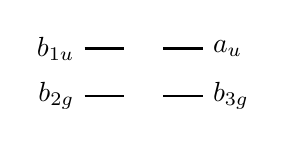
\begin{tikzpicture}[baseline={(current bounding box.center)}]
            % oberste MOs:
            \draw[thick] (0,0) -- (0.5,0)
                node[pos=0, left] {$b_{1u}$}
                ;
            \draw[thick] (1,0) -- (1.5,0)
                node[pos=1, right] {$a_{u}$}
                ;
            % unterste MOs:
            \draw[thick] (0,-0.6) -- (0.5,-0.6)
                node[pos=0, left] {$b_{2g}$}
                ;
            \draw[thick] (1,-0.6) -- (1.5,-0.6)
                node[pos=1, right] {$b_{3g}$}
                ;
        
\end{tikzpicture}
$$
In the following, we will leave out the explicit labeling by orbital symmetry. Each monomer will simply be written as:
$$
\begin{tikzpicture}[baseline={(current bounding box.center)}]
            % oberste MOs:
            \draw[thick] (0,0) -- (0.5,0)
                %node[pos=0, left] {$b_{1u}$}
                ;
            \draw[thick] (1,0) -- (1.5,0)
                %node[pos=1, right] {$a_{u}$}
                ;
            % unterste MOs:
            \draw[thick] (0,-0.6) -- (0.5,-0.6)
                %node[pos=0, left] {$b_{2g}$}
                ;
            \draw[thick] (1,-0.6) -- (1.5,-0.6)
                %node[pos=1, right] {$b_{3g}$}
                ;
        
\end{tikzpicture}
$$
where the character of the orbital is defined by its position. 

Dimer configurations will be written as their monomer occupations, by writing one monomer to the left and one to the right. The orbital order within the group of monomer orbitals follows the above mentioned definition. \\ \\ The transformation of monomer orbitals into dimer orbitals is given by knowing the negative and positive linear combinations of monomer orbitals into dimer orbitals. Transforming this known equation system leads to: 
\begin{subequations}\begin{gather}
a_{u}^{l} = +b_{1g}+a_{u}  \\
b_{1u}^{l} = +a_{g}+b_{1u}  \\
b_{2g}^{l} = +b_{3u}+b_{2g}  \\
b_{3g}^{l} = +b_{2u}+b_{3g}  \\
a_{u}^{r} = -b_{1g}+a_{u}  \\
b_{1u}^{r} = -a_{g}+b_{1u}  \\
b_{2g}^{r} = -b_{3u}+b_{2g}  \\
b_{3g}^{r} = -b_{2u}+b_{3g}\end{gather}\end{subequations}
\newpage

\section{Monomer States and Configurations} 

\[i^3 b_{2u}
\quad = + \left(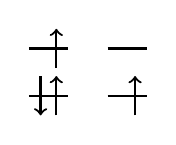
\begin{tikzpicture}[baseline={(current bounding box.center)}]
    % oberste MOs:
    \draw[thick] (0,0) -- (0.5,0); % erster Strich
    \draw[thick] (1,0) -- (1.5,0); % zweiter Strich
    % unterste MOs:
    \draw[thick] (0,-0.6) -- (0.5,-0.6); % dritter Strich
    \draw[thick] (1,-0.6) -- (1.5,-0.6); % vierter Strich
\draw[->, thick] (0.35, -0.25) -- (0.35, 0.25); 
\draw[-> , thick] (0.35, -0.85) -- (0.35, -0.35); 
\draw[<- , thick] (0.15, -0.85) -- (0.15, -0.35); 
 \draw[-> , thick] (1.35, -0.85) -- (1.35, -0.35); 
\end{tikzpicture}\right)-\left(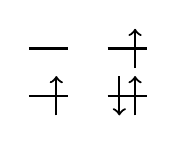
\begin{tikzpicture}[baseline={(current bounding box.center)}]
    % oberste MOs:
    \draw[thick] (0,0) -- (0.5,0); % erster Strich
    \draw[thick] (1,0) -- (1.5,0); % zweiter Strich
    % unterste MOs:
    \draw[thick] (0,-0.6) -- (0.5,-0.6); % dritter Strich
    \draw[thick] (1,-0.6) -- (1.5,-0.6); % vierter Strich
\draw[->, thick] (1.35, -0.25) -- (1.35, 0.25); 
\draw[-> , thick] (0.35, -0.85) -- (0.35, -0.35); 
 \draw[-> , thick] (1.35, -0.85) -- (1.35, -0.35); 
\draw[<- , thick] (1.15, -0.85) -- (1.15, -0.35); 
\end{tikzpicture}\right) \qquad = \left|a2a0\right|-\left|0a2a\right| \]



\[e^3 b_{2u}
\quad = + \left(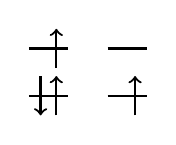
\begin{tikzpicture}[baseline={(current bounding box.center)}]
    % oberste MOs:
    \draw[thick] (0,0) -- (0.5,0); % erster Strich
    \draw[thick] (1,0) -- (1.5,0); % zweiter Strich
    % unterste MOs:
    \draw[thick] (0,-0.6) -- (0.5,-0.6); % dritter Strich
    \draw[thick] (1,-0.6) -- (1.5,-0.6); % vierter Strich
\draw[->, thick] (0.35, -0.25) -- (0.35, 0.25); 
\draw[-> , thick] (0.35, -0.85) -- (0.35, -0.35); 
\draw[<- , thick] (0.15, -0.85) -- (0.15, -0.35); 
 \draw[-> , thick] (1.35, -0.85) -- (1.35, -0.35); 
\end{tikzpicture}\right)+\left(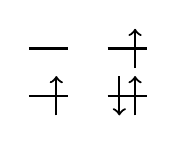
\begin{tikzpicture}[baseline={(current bounding box.center)}]
    % oberste MOs:
    \draw[thick] (0,0) -- (0.5,0); % erster Strich
    \draw[thick] (1,0) -- (1.5,0); % zweiter Strich
    % unterste MOs:
    \draw[thick] (0,-0.6) -- (0.5,-0.6); % dritter Strich
    \draw[thick] (1,-0.6) -- (1.5,-0.6); % vierter Strich
\draw[->, thick] (1.35, -0.25) -- (1.35, 0.25); 
\draw[-> , thick] (0.35, -0.85) -- (0.35, -0.35); 
 \draw[-> , thick] (1.35, -0.85) -- (1.35, -0.35); 
\draw[<- , thick] (1.15, -0.85) -- (1.15, -0.35); 
\end{tikzpicture}\right) \qquad = \left|a2a0\right|+\left|0a2a\right| \]



\[e^3 b_{3u}
\quad = + \left(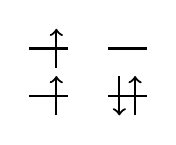
\begin{tikzpicture}[baseline={(current bounding box.center)}]
    % oberste MOs:
    \draw[thick] (0,0) -- (0.5,0); % erster Strich
    \draw[thick] (1,0) -- (1.5,0); % zweiter Strich
    % unterste MOs:
    \draw[thick] (0,-0.6) -- (0.5,-0.6); % dritter Strich
    \draw[thick] (1,-0.6) -- (1.5,-0.6); % vierter Strich
\draw[->, thick] (0.35, -0.25) -- (0.35, 0.25); 
\draw[-> , thick] (0.35, -0.85) -- (0.35, -0.35); 
 \draw[-> , thick] (1.35, -0.85) -- (1.35, -0.35); 
\draw[<- , thick] (1.15, -0.85) -- (1.15, -0.35); 
\end{tikzpicture}\right)-\left(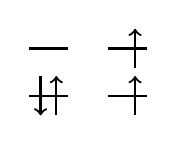
\begin{tikzpicture}[baseline={(current bounding box.center)}]
    % oberste MOs:
    \draw[thick] (0,0) -- (0.5,0); % erster Strich
    \draw[thick] (1,0) -- (1.5,0); % zweiter Strich
    % unterste MOs:
    \draw[thick] (0,-0.6) -- (0.5,-0.6); % dritter Strich
    \draw[thick] (1,-0.6) -- (1.5,-0.6); % vierter Strich
\draw[->, thick] (1.35, -0.25) -- (1.35, 0.25); 
\draw[-> , thick] (0.35, -0.85) -- (0.35, -0.35); 
\draw[<- , thick] (0.15, -0.85) -- (0.15, -0.35); 
 \draw[-> , thick] (1.35, -0.85) -- (1.35, -0.35); 
\end{tikzpicture}\right) \qquad = \left|aa20\right|-\left|02aa\right| \]



\[i^3 b_{3u}
\quad = + \left(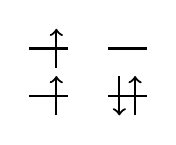
\begin{tikzpicture}[baseline={(current bounding box.center)}]
    % oberste MOs:
    \draw[thick] (0,0) -- (0.5,0); % erster Strich
    \draw[thick] (1,0) -- (1.5,0); % zweiter Strich
    % unterste MOs:
    \draw[thick] (0,-0.6) -- (0.5,-0.6); % dritter Strich
    \draw[thick] (1,-0.6) -- (1.5,-0.6); % vierter Strich
\draw[->, thick] (0.35, -0.25) -- (0.35, 0.25); 
\draw[-> , thick] (0.35, -0.85) -- (0.35, -0.35); 
 \draw[-> , thick] (1.35, -0.85) -- (1.35, -0.35); 
\draw[<- , thick] (1.15, -0.85) -- (1.15, -0.35); 
\end{tikzpicture}\right)+\left(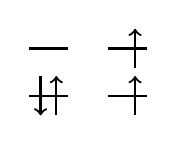
\begin{tikzpicture}[baseline={(current bounding box.center)}]
    % oberste MOs:
    \draw[thick] (0,0) -- (0.5,0); % erster Strich
    \draw[thick] (1,0) -- (1.5,0); % zweiter Strich
    % unterste MOs:
    \draw[thick] (0,-0.6) -- (0.5,-0.6); % dritter Strich
    \draw[thick] (1,-0.6) -- (1.5,-0.6); % vierter Strich
\draw[->, thick] (1.35, -0.25) -- (1.35, 0.25); 
\draw[-> , thick] (0.35, -0.85) -- (0.35, -0.35); 
\draw[<- , thick] (0.15, -0.85) -- (0.15, -0.35); 
 \draw[-> , thick] (1.35, -0.85) -- (1.35, -0.35); 
\end{tikzpicture}\right) \qquad = \left|aa20\right|+\left|02aa\right| \]


\newpage


\section{Linear Combinations: 16 Monomer- / 8 Dimer-States}


\begin{minipage}{\linewidth}
identical $i^3 b_{2u}$ * $i^3 b_{2u}$ \quad = \quad identical $1.3$ * $1.3$
\[ +\left(\text{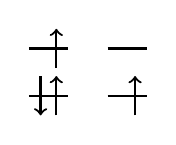
\begin{tikzpicture}[baseline={(current bounding box.center)}]
    % oberste MOs:
    \draw[thick] (0,0) -- (0.5,0); % erster Strich
    \draw[thick] (1,0) -- (1.5,0); % zweiter Strich
    % unterste MOs:
    \draw[thick] (0,-0.6) -- (0.5,-0.6); % dritter Strich
    \draw[thick] (1,-0.6) -- (1.5,-0.6); % vierter Strich
\draw[->, thick] (0.35, -0.25) -- (0.35, 0.25); 
\draw[-> , thick] (0.35, -0.85) -- (0.35, -0.35); 
\draw[<- , thick] (0.15, -0.85) -- (0.15, -0.35); 
 \draw[-> , thick] (1.35, -0.85) -- (1.35, -0.35); 
\end{tikzpicture}\qquad 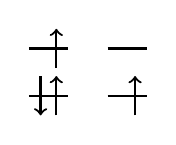
\begin{tikzpicture}[baseline={(current bounding box.center)}]
    % oberste MOs:
    \draw[thick] (0,0) -- (0.5,0); % erster Strich
    \draw[thick] (1,0) -- (1.5,0); % zweiter Strich
    % unterste MOs:
    \draw[thick] (0,-0.6) -- (0.5,-0.6); % dritter Strich
    \draw[thick] (1,-0.6) -- (1.5,-0.6); % vierter Strich
\draw[->, thick] (0.35, -0.25) -- (0.35, 0.25); 
\draw[-> , thick] (0.35, -0.85) -- (0.35, -0.35); 
\draw[<- , thick] (0.15, -0.85) -- (0.15, -0.35); 
 \draw[-> , thick] (1.35, -0.85) -- (1.35, -0.35); 
\end{tikzpicture}}\right)-\left(\text{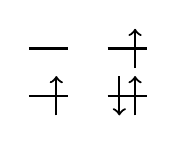
\begin{tikzpicture}[baseline={(current bounding box.center)}]
    % oberste MOs:
    \draw[thick] (0,0) -- (0.5,0); % erster Strich
    \draw[thick] (1,0) -- (1.5,0); % zweiter Strich
    % unterste MOs:
    \draw[thick] (0,-0.6) -- (0.5,-0.6); % dritter Strich
    \draw[thick] (1,-0.6) -- (1.5,-0.6); % vierter Strich
\draw[->, thick] (1.35, -0.25) -- (1.35, 0.25); 
\draw[-> , thick] (0.35, -0.85) -- (0.35, -0.35); 
 \draw[-> , thick] (1.35, -0.85) -- (1.35, -0.35); 
\draw[<- , thick] (1.15, -0.85) -- (1.15, -0.35); 
\end{tikzpicture}\qquad 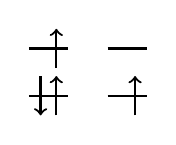
\begin{tikzpicture}[baseline={(current bounding box.center)}]
    % oberste MOs:
    \draw[thick] (0,0) -- (0.5,0); % erster Strich
    \draw[thick] (1,0) -- (1.5,0); % zweiter Strich
    % unterste MOs:
    \draw[thick] (0,-0.6) -- (0.5,-0.6); % dritter Strich
    \draw[thick] (1,-0.6) -- (1.5,-0.6); % vierter Strich
\draw[->, thick] (0.35, -0.25) -- (0.35, 0.25); 
\draw[-> , thick] (0.35, -0.85) -- (0.35, -0.35); 
\draw[<- , thick] (0.15, -0.85) -- (0.15, -0.35); 
 \draw[-> , thick] (1.35, -0.85) -- (1.35, -0.35); 
\end{tikzpicture}}\right)-\left(\text{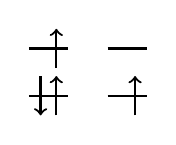
\begin{tikzpicture}[baseline={(current bounding box.center)}]
    % oberste MOs:
    \draw[thick] (0,0) -- (0.5,0); % erster Strich
    \draw[thick] (1,0) -- (1.5,0); % zweiter Strich
    % unterste MOs:
    \draw[thick] (0,-0.6) -- (0.5,-0.6); % dritter Strich
    \draw[thick] (1,-0.6) -- (1.5,-0.6); % vierter Strich
\draw[->, thick] (0.35, -0.25) -- (0.35, 0.25); 
\draw[-> , thick] (0.35, -0.85) -- (0.35, -0.35); 
\draw[<- , thick] (0.15, -0.85) -- (0.15, -0.35); 
 \draw[-> , thick] (1.35, -0.85) -- (1.35, -0.35); 
\end{tikzpicture}\qquad 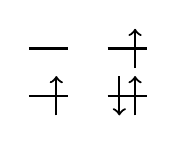
\begin{tikzpicture}[baseline={(current bounding box.center)}]
    % oberste MOs:
    \draw[thick] (0,0) -- (0.5,0); % erster Strich
    \draw[thick] (1,0) -- (1.5,0); % zweiter Strich
    % unterste MOs:
    \draw[thick] (0,-0.6) -- (0.5,-0.6); % dritter Strich
    \draw[thick] (1,-0.6) -- (1.5,-0.6); % vierter Strich
\draw[->, thick] (1.35, -0.25) -- (1.35, 0.25); 
\draw[-> , thick] (0.35, -0.85) -- (0.35, -0.35); 
 \draw[-> , thick] (1.35, -0.85) -- (1.35, -0.35); 
\draw[<- , thick] (1.15, -0.85) -- (1.15, -0.35); 
\end{tikzpicture}}\right)+\left(\text{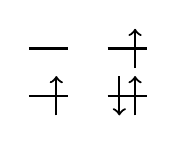
\begin{tikzpicture}[baseline={(current bounding box.center)}]
    % oberste MOs:
    \draw[thick] (0,0) -- (0.5,0); % erster Strich
    \draw[thick] (1,0) -- (1.5,0); % zweiter Strich
    % unterste MOs:
    \draw[thick] (0,-0.6) -- (0.5,-0.6); % dritter Strich
    \draw[thick] (1,-0.6) -- (1.5,-0.6); % vierter Strich
\draw[->, thick] (1.35, -0.25) -- (1.35, 0.25); 
\draw[-> , thick] (0.35, -0.85) -- (0.35, -0.35); 
 \draw[-> , thick] (1.35, -0.85) -- (1.35, -0.35); 
\draw[<- , thick] (1.15, -0.85) -- (1.15, -0.35); 
\end{tikzpicture}\qquad 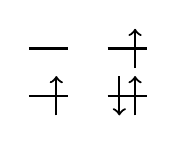
\begin{tikzpicture}[baseline={(current bounding box.center)}]
    % oberste MOs:
    \draw[thick] (0,0) -- (0.5,0); % erster Strich
    \draw[thick] (1,0) -- (1.5,0); % zweiter Strich
    % unterste MOs:
    \draw[thick] (0,-0.6) -- (0.5,-0.6); % dritter Strich
    \draw[thick] (1,-0.6) -- (1.5,-0.6); % vierter Strich
\draw[->, thick] (1.35, -0.25) -- (1.35, 0.25); 
\draw[-> , thick] (0.35, -0.85) -- (0.35, -0.35); 
 \draw[-> , thick] (1.35, -0.85) -- (1.35, -0.35); 
\draw[<- , thick] (1.15, -0.85) -- (1.15, -0.35); 
\end{tikzpicture}}\right)\\\\\]


written in CI Vectors: 
 $$+ 1 \cdot \left|a2a0 \right| \cdot \left| a2a0 \right| 
- 1 \cdot \left|0a2a \right| \cdot \left| a2a0 \right| 
- 1 \cdot \left|a2a0 \right| \cdot \left| 0a2a \right| 
+ 1 \cdot \left|0a2a \right| \cdot \left| 0a2a \right| 
$$



 forms the following possible dimer combinations:

$$+ 1 \cdot \left|a2a0a2a0 \right| + 1 \cdot \left|0a2a0a2a \right| - \frac{1}{8} \cdot \left|0a2aa2a0 \right| + \frac{1}{8} \cdot \left|0a20a2aa \right| + \frac{1}{8} \cdot \left|0aaaa220 \right| - \frac{1}{8} \cdot \left|0aa0a22a \right|  $$ $$ + \frac{1}{8} \cdot \left|022aaaa0 \right| - \frac{1}{8} \cdot \left|0220aaaa \right| - \frac{1}{8} \cdot \left|02aaaa20 \right| + \frac{1}{8} \cdot \left|02a0aa2a \right| + \frac{1}{8} \cdot \left|aa2a02a0 \right| - \frac{1}{8} \cdot \left|aa2002aa \right|  $$ $$ - \frac{1}{8} \cdot \left|aaaa0220 \right| + \frac{1}{8} \cdot \left|aaa0022a \right| - \frac{1}{8} \cdot \left|a22a0aa0 \right| + \frac{1}{8} \cdot \left|a2200aaa \right| + \frac{1}{8} \cdot \left|a2aa0a20 \right| - \frac{1}{8} \cdot \left|a2a00a2a \right| $$



\end{minipage}
\vspace{0.5cm}


or, expressed in terms of symmetry:\begin{multline*}
=-4\left|\underbrace{a_{g} b_{2u} b_{1u} b_{3g}}_{a_{g}}\right|-2\left|\underbrace{a_{g} b_{3u} b_{2u} b_{1g}}_{a_{g}}\right|+2\left|\underbrace{a_{g} b_{3u} b_{3g} a_{u}}_{a_{g}}\right|+2\left|\underbrace{a_{g} b_{2u} b_{2g} a_{u}}_{a_{g}}\right|\\
+2\left|\underbrace{a_{g} b_{1g} b_{2g} b_{3g}}_{a_{g}}\right|+2\left|\underbrace{b_{3u} b_{2u} b_{1u} a_{u}}_{a_{g}}\right|+2\left|\underbrace{b_{3u} b_{1g} b_{1u} b_{3g}}_{a_{g}}\right|+2\left|\underbrace{b_{2u} b_{1g} b_{1u} b_{2g}}_{a_{g}}\right|\\
-2\left|\underbrace{b_{1u} b_{2g} b_{3g} a_{u}}_{a_{g}}\right|-4\left|\underbrace{b_{3u} b_{1g} b_{2g} a_{u}}_{a_{g}}\right|
\end{multline*}\\\\

 


\hrule
\vspace{0.5cm}



\begin{minipage}{\linewidth}
plus combination: $i^3 b_{2u}$ * $e^3 b_{2u}$ + $e^3 b_{2u}$ * $i^3 b_{2u}$  \quad = \quad plus combination: $1.3$ * $2.3$ + $2.3$ * $1.3$ 
\[ \begin{array}{c}+\left(\text{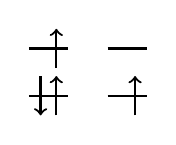
\begin{tikzpicture}[baseline={(current bounding box.center)}]
    % oberste MOs:
    \draw[thick] (0,0) -- (0.5,0); % erster Strich
    \draw[thick] (1,0) -- (1.5,0); % zweiter Strich
    % unterste MOs:
    \draw[thick] (0,-0.6) -- (0.5,-0.6); % dritter Strich
    \draw[thick] (1,-0.6) -- (1.5,-0.6); % vierter Strich
\draw[->, thick] (0.35, -0.25) -- (0.35, 0.25); 
\draw[-> , thick] (0.35, -0.85) -- (0.35, -0.35); 
\draw[<- , thick] (0.15, -0.85) -- (0.15, -0.35); 
 \draw[-> , thick] (1.35, -0.85) -- (1.35, -0.35); 
\end{tikzpicture}\qquad 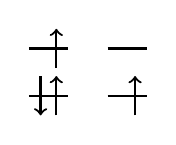
\begin{tikzpicture}[baseline={(current bounding box.center)}]
    % oberste MOs:
    \draw[thick] (0,0) -- (0.5,0); % erster Strich
    \draw[thick] (1,0) -- (1.5,0); % zweiter Strich
    % unterste MOs:
    \draw[thick] (0,-0.6) -- (0.5,-0.6); % dritter Strich
    \draw[thick] (1,-0.6) -- (1.5,-0.6); % vierter Strich
\draw[->, thick] (0.35, -0.25) -- (0.35, 0.25); 
\draw[-> , thick] (0.35, -0.85) -- (0.35, -0.35); 
\draw[<- , thick] (0.15, -0.85) -- (0.15, -0.35); 
 \draw[-> , thick] (1.35, -0.85) -- (1.35, -0.35); 
\end{tikzpicture}}\right)-\left(\text{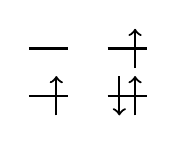
\begin{tikzpicture}[baseline={(current bounding box.center)}]
    % oberste MOs:
    \draw[thick] (0,0) -- (0.5,0); % erster Strich
    \draw[thick] (1,0) -- (1.5,0); % zweiter Strich
    % unterste MOs:
    \draw[thick] (0,-0.6) -- (0.5,-0.6); % dritter Strich
    \draw[thick] (1,-0.6) -- (1.5,-0.6); % vierter Strich
\draw[->, thick] (1.35, -0.25) -- (1.35, 0.25); 
\draw[-> , thick] (0.35, -0.85) -- (0.35, -0.35); 
 \draw[-> , thick] (1.35, -0.85) -- (1.35, -0.35); 
\draw[<- , thick] (1.15, -0.85) -- (1.15, -0.35); 
\end{tikzpicture}\qquad 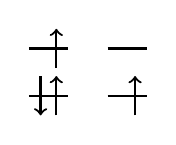
\begin{tikzpicture}[baseline={(current bounding box.center)}]
    % oberste MOs:
    \draw[thick] (0,0) -- (0.5,0); % erster Strich
    \draw[thick] (1,0) -- (1.5,0); % zweiter Strich
    % unterste MOs:
    \draw[thick] (0,-0.6) -- (0.5,-0.6); % dritter Strich
    \draw[thick] (1,-0.6) -- (1.5,-0.6); % vierter Strich
\draw[->, thick] (0.35, -0.25) -- (0.35, 0.25); 
\draw[-> , thick] (0.35, -0.85) -- (0.35, -0.35); 
\draw[<- , thick] (0.15, -0.85) -- (0.15, -0.35); 
 \draw[-> , thick] (1.35, -0.85) -- (1.35, -0.35); 
\end{tikzpicture}}\right)+\left(\text{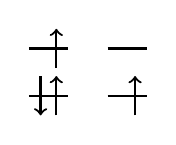
\begin{tikzpicture}[baseline={(current bounding box.center)}]
    % oberste MOs:
    \draw[thick] (0,0) -- (0.5,0); % erster Strich
    \draw[thick] (1,0) -- (1.5,0); % zweiter Strich
    % unterste MOs:
    \draw[thick] (0,-0.6) -- (0.5,-0.6); % dritter Strich
    \draw[thick] (1,-0.6) -- (1.5,-0.6); % vierter Strich
\draw[->, thick] (0.35, -0.25) -- (0.35, 0.25); 
\draw[-> , thick] (0.35, -0.85) -- (0.35, -0.35); 
\draw[<- , thick] (0.15, -0.85) -- (0.15, -0.35); 
 \draw[-> , thick] (1.35, -0.85) -- (1.35, -0.35); 
\end{tikzpicture}\qquad 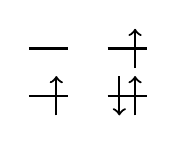
\begin{tikzpicture}[baseline={(current bounding box.center)}]
    % oberste MOs:
    \draw[thick] (0,0) -- (0.5,0); % erster Strich
    \draw[thick] (1,0) -- (1.5,0); % zweiter Strich
    % unterste MOs:
    \draw[thick] (0,-0.6) -- (0.5,-0.6); % dritter Strich
    \draw[thick] (1,-0.6) -- (1.5,-0.6); % vierter Strich
\draw[->, thick] (1.35, -0.25) -- (1.35, 0.25); 
\draw[-> , thick] (0.35, -0.85) -- (0.35, -0.35); 
 \draw[-> , thick] (1.35, -0.85) -- (1.35, -0.35); 
\draw[<- , thick] (1.15, -0.85) -- (1.15, -0.35); 
\end{tikzpicture}}\right)-\left(\text{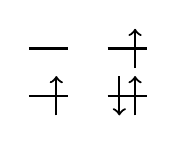
\begin{tikzpicture}[baseline={(current bounding box.center)}]
    % oberste MOs:
    \draw[thick] (0,0) -- (0.5,0); % erster Strich
    \draw[thick] (1,0) -- (1.5,0); % zweiter Strich
    % unterste MOs:
    \draw[thick] (0,-0.6) -- (0.5,-0.6); % dritter Strich
    \draw[thick] (1,-0.6) -- (1.5,-0.6); % vierter Strich
\draw[->, thick] (1.35, -0.25) -- (1.35, 0.25); 
\draw[-> , thick] (0.35, -0.85) -- (0.35, -0.35); 
 \draw[-> , thick] (1.35, -0.85) -- (1.35, -0.35); 
\draw[<- , thick] (1.15, -0.85) -- (1.15, -0.35); 
\end{tikzpicture}\qquad 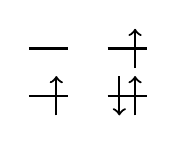
\begin{tikzpicture}[baseline={(current bounding box.center)}]
    % oberste MOs:
    \draw[thick] (0,0) -- (0.5,0); % erster Strich
    \draw[thick] (1,0) -- (1.5,0); % zweiter Strich
    % unterste MOs:
    \draw[thick] (0,-0.6) -- (0.5,-0.6); % dritter Strich
    \draw[thick] (1,-0.6) -- (1.5,-0.6); % vierter Strich
\draw[->, thick] (1.35, -0.25) -- (1.35, 0.25); 
\draw[-> , thick] (0.35, -0.85) -- (0.35, -0.35); 
 \draw[-> , thick] (1.35, -0.85) -- (1.35, -0.35); 
\draw[<- , thick] (1.15, -0.85) -- (1.15, -0.35); 
\end{tikzpicture}}\right)\\\\+\left(\text{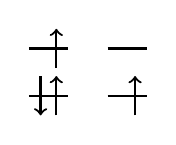
\begin{tikzpicture}[baseline={(current bounding box.center)}]
    % oberste MOs:
    \draw[thick] (0,0) -- (0.5,0); % erster Strich
    \draw[thick] (1,0) -- (1.5,0); % zweiter Strich
    % unterste MOs:
    \draw[thick] (0,-0.6) -- (0.5,-0.6); % dritter Strich
    \draw[thick] (1,-0.6) -- (1.5,-0.6); % vierter Strich
\draw[->, thick] (0.35, -0.25) -- (0.35, 0.25); 
\draw[-> , thick] (0.35, -0.85) -- (0.35, -0.35); 
\draw[<- , thick] (0.15, -0.85) -- (0.15, -0.35); 
 \draw[-> , thick] (1.35, -0.85) -- (1.35, -0.35); 
\end{tikzpicture}\qquad 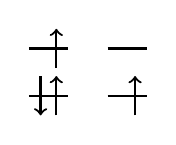
\begin{tikzpicture}[baseline={(current bounding box.center)}]
    % oberste MOs:
    \draw[thick] (0,0) -- (0.5,0); % erster Strich
    \draw[thick] (1,0) -- (1.5,0); % zweiter Strich
    % unterste MOs:
    \draw[thick] (0,-0.6) -- (0.5,-0.6); % dritter Strich
    \draw[thick] (1,-0.6) -- (1.5,-0.6); % vierter Strich
\draw[->, thick] (0.35, -0.25) -- (0.35, 0.25); 
\draw[-> , thick] (0.35, -0.85) -- (0.35, -0.35); 
\draw[<- , thick] (0.15, -0.85) -- (0.15, -0.35); 
 \draw[-> , thick] (1.35, -0.85) -- (1.35, -0.35); 
\end{tikzpicture}}\right)+\left(\text{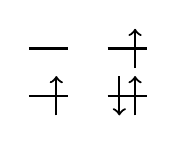
\begin{tikzpicture}[baseline={(current bounding box.center)}]
    % oberste MOs:
    \draw[thick] (0,0) -- (0.5,0); % erster Strich
    \draw[thick] (1,0) -- (1.5,0); % zweiter Strich
    % unterste MOs:
    \draw[thick] (0,-0.6) -- (0.5,-0.6); % dritter Strich
    \draw[thick] (1,-0.6) -- (1.5,-0.6); % vierter Strich
\draw[->, thick] (1.35, -0.25) -- (1.35, 0.25); 
\draw[-> , thick] (0.35, -0.85) -- (0.35, -0.35); 
 \draw[-> , thick] (1.35, -0.85) -- (1.35, -0.35); 
\draw[<- , thick] (1.15, -0.85) -- (1.15, -0.35); 
\end{tikzpicture}\qquad 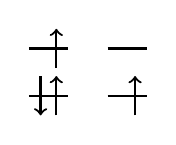
\begin{tikzpicture}[baseline={(current bounding box.center)}]
    % oberste MOs:
    \draw[thick] (0,0) -- (0.5,0); % erster Strich
    \draw[thick] (1,0) -- (1.5,0); % zweiter Strich
    % unterste MOs:
    \draw[thick] (0,-0.6) -- (0.5,-0.6); % dritter Strich
    \draw[thick] (1,-0.6) -- (1.5,-0.6); % vierter Strich
\draw[->, thick] (0.35, -0.25) -- (0.35, 0.25); 
\draw[-> , thick] (0.35, -0.85) -- (0.35, -0.35); 
\draw[<- , thick] (0.15, -0.85) -- (0.15, -0.35); 
 \draw[-> , thick] (1.35, -0.85) -- (1.35, -0.35); 
\end{tikzpicture}}\right)-\left(\text{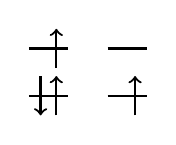
\begin{tikzpicture}[baseline={(current bounding box.center)}]
    % oberste MOs:
    \draw[thick] (0,0) -- (0.5,0); % erster Strich
    \draw[thick] (1,0) -- (1.5,0); % zweiter Strich
    % unterste MOs:
    \draw[thick] (0,-0.6) -- (0.5,-0.6); % dritter Strich
    \draw[thick] (1,-0.6) -- (1.5,-0.6); % vierter Strich
\draw[->, thick] (0.35, -0.25) -- (0.35, 0.25); 
\draw[-> , thick] (0.35, -0.85) -- (0.35, -0.35); 
\draw[<- , thick] (0.15, -0.85) -- (0.15, -0.35); 
 \draw[-> , thick] (1.35, -0.85) -- (1.35, -0.35); 
\end{tikzpicture}\qquad 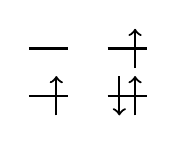
\begin{tikzpicture}[baseline={(current bounding box.center)}]
    % oberste MOs:
    \draw[thick] (0,0) -- (0.5,0); % erster Strich
    \draw[thick] (1,0) -- (1.5,0); % zweiter Strich
    % unterste MOs:
    \draw[thick] (0,-0.6) -- (0.5,-0.6); % dritter Strich
    \draw[thick] (1,-0.6) -- (1.5,-0.6); % vierter Strich
\draw[->, thick] (1.35, -0.25) -- (1.35, 0.25); 
\draw[-> , thick] (0.35, -0.85) -- (0.35, -0.35); 
 \draw[-> , thick] (1.35, -0.85) -- (1.35, -0.35); 
\draw[<- , thick] (1.15, -0.85) -- (1.15, -0.35); 
\end{tikzpicture}}\right)-\left(\text{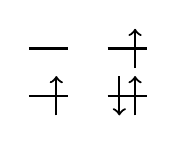
\begin{tikzpicture}[baseline={(current bounding box.center)}]
    % oberste MOs:
    \draw[thick] (0,0) -- (0.5,0); % erster Strich
    \draw[thick] (1,0) -- (1.5,0); % zweiter Strich
    % unterste MOs:
    \draw[thick] (0,-0.6) -- (0.5,-0.6); % dritter Strich
    \draw[thick] (1,-0.6) -- (1.5,-0.6); % vierter Strich
\draw[->, thick] (1.35, -0.25) -- (1.35, 0.25); 
\draw[-> , thick] (0.35, -0.85) -- (0.35, -0.35); 
 \draw[-> , thick] (1.35, -0.85) -- (1.35, -0.35); 
\draw[<- , thick] (1.15, -0.85) -- (1.15, -0.35); 
\end{tikzpicture}\qquad 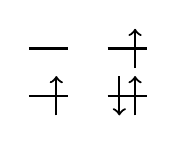
\begin{tikzpicture}[baseline={(current bounding box.center)}]
    % oberste MOs:
    \draw[thick] (0,0) -- (0.5,0); % erster Strich
    \draw[thick] (1,0) -- (1.5,0); % zweiter Strich
    % unterste MOs:
    \draw[thick] (0,-0.6) -- (0.5,-0.6); % dritter Strich
    \draw[thick] (1,-0.6) -- (1.5,-0.6); % vierter Strich
\draw[->, thick] (1.35, -0.25) -- (1.35, 0.25); 
\draw[-> , thick] (0.35, -0.85) -- (0.35, -0.35); 
 \draw[-> , thick] (1.35, -0.85) -- (1.35, -0.35); 
\draw[<- , thick] (1.15, -0.85) -- (1.15, -0.35); 
\end{tikzpicture}}\right)\\\\\end{array}\]


written in CI Vectors: 
 $$+ 1 \cdot \left|a2a0 \right| \cdot \left| a2a0 \right| 
- 1 \cdot \left|0a2a \right| \cdot \left| a2a0 \right| 
+ 1 \cdot \left|a2a0 \right| \cdot \left| 0a2a \right| 
- 1 \cdot \left|0a2a \right| \cdot \left| 0a2a \right| 
 $$ $$ + 1 \cdot \left|a2a0 \right| \cdot \left| a2a0 \right| 
+ 1 \cdot \left|0a2a \right| \cdot \left| a2a0 \right| 
- 1 \cdot \left|a2a0 \right| \cdot \left| 0a2a \right| 
- 1 \cdot \left|0a2a \right| \cdot \left| 0a2a \right| 
$$



 forms the following possible dimer combinations:

$$+ 2 \cdot \left|a2a0a2a0 \right| - 2 \cdot \left|0a2a0a2a \right| $$



\end{minipage}
\vspace{0.5cm}


or, expressed in terms of symmetry:\begin{multline*}
=-8\left|\underbrace{a_{g} b_{2u} b_{1u} b_{3g}}_{a_{g}}\right|+8\left|\underbrace{b_{3u} b_{1g} b_{2g} a_{u}}_{a_{g}}\right|
\end{multline*}\\\\

 


\hrule
\vspace{0.5cm}



\begin{minipage}{\linewidth}
minus combination: $i^3 b_{2u}$ * $e^3 b_{2u}$ - $e^3 b_{2u}$ * $i^3 b_{2u}$  \quad = \quad minus combination: $1.3$ * $2.3$ - $2.3$ * $1.3$ 
\[ \begin{array}{c}+\left(\text{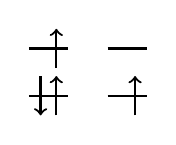
\begin{tikzpicture}[baseline={(current bounding box.center)}]
    % oberste MOs:
    \draw[thick] (0,0) -- (0.5,0); % erster Strich
    \draw[thick] (1,0) -- (1.5,0); % zweiter Strich
    % unterste MOs:
    \draw[thick] (0,-0.6) -- (0.5,-0.6); % dritter Strich
    \draw[thick] (1,-0.6) -- (1.5,-0.6); % vierter Strich
\draw[->, thick] (0.35, -0.25) -- (0.35, 0.25); 
\draw[-> , thick] (0.35, -0.85) -- (0.35, -0.35); 
\draw[<- , thick] (0.15, -0.85) -- (0.15, -0.35); 
 \draw[-> , thick] (1.35, -0.85) -- (1.35, -0.35); 
\end{tikzpicture}\qquad 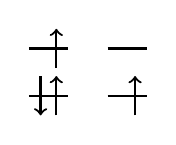
\begin{tikzpicture}[baseline={(current bounding box.center)}]
    % oberste MOs:
    \draw[thick] (0,0) -- (0.5,0); % erster Strich
    \draw[thick] (1,0) -- (1.5,0); % zweiter Strich
    % unterste MOs:
    \draw[thick] (0,-0.6) -- (0.5,-0.6); % dritter Strich
    \draw[thick] (1,-0.6) -- (1.5,-0.6); % vierter Strich
\draw[->, thick] (0.35, -0.25) -- (0.35, 0.25); 
\draw[-> , thick] (0.35, -0.85) -- (0.35, -0.35); 
\draw[<- , thick] (0.15, -0.85) -- (0.15, -0.35); 
 \draw[-> , thick] (1.35, -0.85) -- (1.35, -0.35); 
\end{tikzpicture}}\right)-\left(\text{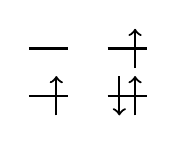
\begin{tikzpicture}[baseline={(current bounding box.center)}]
    % oberste MOs:
    \draw[thick] (0,0) -- (0.5,0); % erster Strich
    \draw[thick] (1,0) -- (1.5,0); % zweiter Strich
    % unterste MOs:
    \draw[thick] (0,-0.6) -- (0.5,-0.6); % dritter Strich
    \draw[thick] (1,-0.6) -- (1.5,-0.6); % vierter Strich
\draw[->, thick] (1.35, -0.25) -- (1.35, 0.25); 
\draw[-> , thick] (0.35, -0.85) -- (0.35, -0.35); 
 \draw[-> , thick] (1.35, -0.85) -- (1.35, -0.35); 
\draw[<- , thick] (1.15, -0.85) -- (1.15, -0.35); 
\end{tikzpicture}\qquad 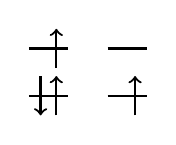
\begin{tikzpicture}[baseline={(current bounding box.center)}]
    % oberste MOs:
    \draw[thick] (0,0) -- (0.5,0); % erster Strich
    \draw[thick] (1,0) -- (1.5,0); % zweiter Strich
    % unterste MOs:
    \draw[thick] (0,-0.6) -- (0.5,-0.6); % dritter Strich
    \draw[thick] (1,-0.6) -- (1.5,-0.6); % vierter Strich
\draw[->, thick] (0.35, -0.25) -- (0.35, 0.25); 
\draw[-> , thick] (0.35, -0.85) -- (0.35, -0.35); 
\draw[<- , thick] (0.15, -0.85) -- (0.15, -0.35); 
 \draw[-> , thick] (1.35, -0.85) -- (1.35, -0.35); 
\end{tikzpicture}}\right)+\left(\text{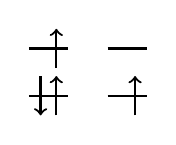
\begin{tikzpicture}[baseline={(current bounding box.center)}]
    % oberste MOs:
    \draw[thick] (0,0) -- (0.5,0); % erster Strich
    \draw[thick] (1,0) -- (1.5,0); % zweiter Strich
    % unterste MOs:
    \draw[thick] (0,-0.6) -- (0.5,-0.6); % dritter Strich
    \draw[thick] (1,-0.6) -- (1.5,-0.6); % vierter Strich
\draw[->, thick] (0.35, -0.25) -- (0.35, 0.25); 
\draw[-> , thick] (0.35, -0.85) -- (0.35, -0.35); 
\draw[<- , thick] (0.15, -0.85) -- (0.15, -0.35); 
 \draw[-> , thick] (1.35, -0.85) -- (1.35, -0.35); 
\end{tikzpicture}\qquad 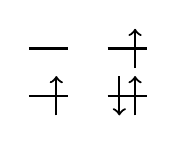
\begin{tikzpicture}[baseline={(current bounding box.center)}]
    % oberste MOs:
    \draw[thick] (0,0) -- (0.5,0); % erster Strich
    \draw[thick] (1,0) -- (1.5,0); % zweiter Strich
    % unterste MOs:
    \draw[thick] (0,-0.6) -- (0.5,-0.6); % dritter Strich
    \draw[thick] (1,-0.6) -- (1.5,-0.6); % vierter Strich
\draw[->, thick] (1.35, -0.25) -- (1.35, 0.25); 
\draw[-> , thick] (0.35, -0.85) -- (0.35, -0.35); 
 \draw[-> , thick] (1.35, -0.85) -- (1.35, -0.35); 
\draw[<- , thick] (1.15, -0.85) -- (1.15, -0.35); 
\end{tikzpicture}}\right)-\left(\text{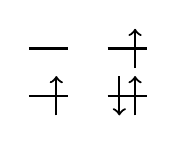
\begin{tikzpicture}[baseline={(current bounding box.center)}]
    % oberste MOs:
    \draw[thick] (0,0) -- (0.5,0); % erster Strich
    \draw[thick] (1,0) -- (1.5,0); % zweiter Strich
    % unterste MOs:
    \draw[thick] (0,-0.6) -- (0.5,-0.6); % dritter Strich
    \draw[thick] (1,-0.6) -- (1.5,-0.6); % vierter Strich
\draw[->, thick] (1.35, -0.25) -- (1.35, 0.25); 
\draw[-> , thick] (0.35, -0.85) -- (0.35, -0.35); 
 \draw[-> , thick] (1.35, -0.85) -- (1.35, -0.35); 
\draw[<- , thick] (1.15, -0.85) -- (1.15, -0.35); 
\end{tikzpicture}\qquad 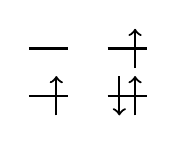
\begin{tikzpicture}[baseline={(current bounding box.center)}]
    % oberste MOs:
    \draw[thick] (0,0) -- (0.5,0); % erster Strich
    \draw[thick] (1,0) -- (1.5,0); % zweiter Strich
    % unterste MOs:
    \draw[thick] (0,-0.6) -- (0.5,-0.6); % dritter Strich
    \draw[thick] (1,-0.6) -- (1.5,-0.6); % vierter Strich
\draw[->, thick] (1.35, -0.25) -- (1.35, 0.25); 
\draw[-> , thick] (0.35, -0.85) -- (0.35, -0.35); 
 \draw[-> , thick] (1.35, -0.85) -- (1.35, -0.35); 
\draw[<- , thick] (1.15, -0.85) -- (1.15, -0.35); 
\end{tikzpicture}}\right)\\\\-\left(\text{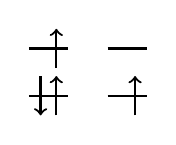
\begin{tikzpicture}[baseline={(current bounding box.center)}]
    % oberste MOs:
    \draw[thick] (0,0) -- (0.5,0); % erster Strich
    \draw[thick] (1,0) -- (1.5,0); % zweiter Strich
    % unterste MOs:
    \draw[thick] (0,-0.6) -- (0.5,-0.6); % dritter Strich
    \draw[thick] (1,-0.6) -- (1.5,-0.6); % vierter Strich
\draw[->, thick] (0.35, -0.25) -- (0.35, 0.25); 
\draw[-> , thick] (0.35, -0.85) -- (0.35, -0.35); 
\draw[<- , thick] (0.15, -0.85) -- (0.15, -0.35); 
 \draw[-> , thick] (1.35, -0.85) -- (1.35, -0.35); 
\end{tikzpicture}\qquad 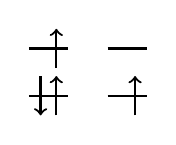
\begin{tikzpicture}[baseline={(current bounding box.center)}]
    % oberste MOs:
    \draw[thick] (0,0) -- (0.5,0); % erster Strich
    \draw[thick] (1,0) -- (1.5,0); % zweiter Strich
    % unterste MOs:
    \draw[thick] (0,-0.6) -- (0.5,-0.6); % dritter Strich
    \draw[thick] (1,-0.6) -- (1.5,-0.6); % vierter Strich
\draw[->, thick] (0.35, -0.25) -- (0.35, 0.25); 
\draw[-> , thick] (0.35, -0.85) -- (0.35, -0.35); 
\draw[<- , thick] (0.15, -0.85) -- (0.15, -0.35); 
 \draw[-> , thick] (1.35, -0.85) -- (1.35, -0.35); 
\end{tikzpicture}}\right)-\left(\text{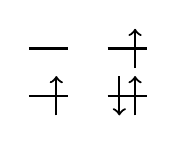
\begin{tikzpicture}[baseline={(current bounding box.center)}]
    % oberste MOs:
    \draw[thick] (0,0) -- (0.5,0); % erster Strich
    \draw[thick] (1,0) -- (1.5,0); % zweiter Strich
    % unterste MOs:
    \draw[thick] (0,-0.6) -- (0.5,-0.6); % dritter Strich
    \draw[thick] (1,-0.6) -- (1.5,-0.6); % vierter Strich
\draw[->, thick] (1.35, -0.25) -- (1.35, 0.25); 
\draw[-> , thick] (0.35, -0.85) -- (0.35, -0.35); 
 \draw[-> , thick] (1.35, -0.85) -- (1.35, -0.35); 
\draw[<- , thick] (1.15, -0.85) -- (1.15, -0.35); 
\end{tikzpicture}\qquad 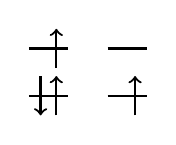
\begin{tikzpicture}[baseline={(current bounding box.center)}]
    % oberste MOs:
    \draw[thick] (0,0) -- (0.5,0); % erster Strich
    \draw[thick] (1,0) -- (1.5,0); % zweiter Strich
    % unterste MOs:
    \draw[thick] (0,-0.6) -- (0.5,-0.6); % dritter Strich
    \draw[thick] (1,-0.6) -- (1.5,-0.6); % vierter Strich
\draw[->, thick] (0.35, -0.25) -- (0.35, 0.25); 
\draw[-> , thick] (0.35, -0.85) -- (0.35, -0.35); 
\draw[<- , thick] (0.15, -0.85) -- (0.15, -0.35); 
 \draw[-> , thick] (1.35, -0.85) -- (1.35, -0.35); 
\end{tikzpicture}}\right)+\left(\text{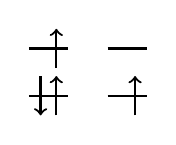
\begin{tikzpicture}[baseline={(current bounding box.center)}]
    % oberste MOs:
    \draw[thick] (0,0) -- (0.5,0); % erster Strich
    \draw[thick] (1,0) -- (1.5,0); % zweiter Strich
    % unterste MOs:
    \draw[thick] (0,-0.6) -- (0.5,-0.6); % dritter Strich
    \draw[thick] (1,-0.6) -- (1.5,-0.6); % vierter Strich
\draw[->, thick] (0.35, -0.25) -- (0.35, 0.25); 
\draw[-> , thick] (0.35, -0.85) -- (0.35, -0.35); 
\draw[<- , thick] (0.15, -0.85) -- (0.15, -0.35); 
 \draw[-> , thick] (1.35, -0.85) -- (1.35, -0.35); 
\end{tikzpicture}\qquad 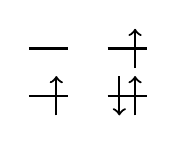
\begin{tikzpicture}[baseline={(current bounding box.center)}]
    % oberste MOs:
    \draw[thick] (0,0) -- (0.5,0); % erster Strich
    \draw[thick] (1,0) -- (1.5,0); % zweiter Strich
    % unterste MOs:
    \draw[thick] (0,-0.6) -- (0.5,-0.6); % dritter Strich
    \draw[thick] (1,-0.6) -- (1.5,-0.6); % vierter Strich
\draw[->, thick] (1.35, -0.25) -- (1.35, 0.25); 
\draw[-> , thick] (0.35, -0.85) -- (0.35, -0.35); 
 \draw[-> , thick] (1.35, -0.85) -- (1.35, -0.35); 
\draw[<- , thick] (1.15, -0.85) -- (1.15, -0.35); 
\end{tikzpicture}}\right)+\left(\text{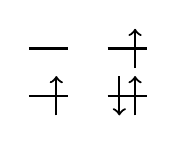
\begin{tikzpicture}[baseline={(current bounding box.center)}]
    % oberste MOs:
    \draw[thick] (0,0) -- (0.5,0); % erster Strich
    \draw[thick] (1,0) -- (1.5,0); % zweiter Strich
    % unterste MOs:
    \draw[thick] (0,-0.6) -- (0.5,-0.6); % dritter Strich
    \draw[thick] (1,-0.6) -- (1.5,-0.6); % vierter Strich
\draw[->, thick] (1.35, -0.25) -- (1.35, 0.25); 
\draw[-> , thick] (0.35, -0.85) -- (0.35, -0.35); 
 \draw[-> , thick] (1.35, -0.85) -- (1.35, -0.35); 
\draw[<- , thick] (1.15, -0.85) -- (1.15, -0.35); 
\end{tikzpicture}\qquad 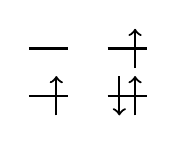
\begin{tikzpicture}[baseline={(current bounding box.center)}]
    % oberste MOs:
    \draw[thick] (0,0) -- (0.5,0); % erster Strich
    \draw[thick] (1,0) -- (1.5,0); % zweiter Strich
    % unterste MOs:
    \draw[thick] (0,-0.6) -- (0.5,-0.6); % dritter Strich
    \draw[thick] (1,-0.6) -- (1.5,-0.6); % vierter Strich
\draw[->, thick] (1.35, -0.25) -- (1.35, 0.25); 
\draw[-> , thick] (0.35, -0.85) -- (0.35, -0.35); 
 \draw[-> , thick] (1.35, -0.85) -- (1.35, -0.35); 
\draw[<- , thick] (1.15, -0.85) -- (1.15, -0.35); 
\end{tikzpicture}}\right)\\\\\end{array}\]


written in CI Vectors: 
 $$+ 1 \cdot \left|a2a0 \right| \cdot \left| a2a0 \right| 
- 1 \cdot \left|0a2a \right| \cdot \left| a2a0 \right| 
+ 1 \cdot \left|a2a0 \right| \cdot \left| 0a2a \right| 
- 1 \cdot \left|0a2a \right| \cdot \left| 0a2a \right| 
 $$ $$ - 1 \cdot \left|a2a0 \right| \cdot \left| a2a0 \right| 
- 1 \cdot \left|0a2a \right| \cdot \left| a2a0 \right| 
+ 1 \cdot \left|a2a0 \right| \cdot \left| 0a2a \right| 
+ 1 \cdot \left|0a2a \right| \cdot \left| 0a2a \right| 
$$



 forms the following possible dimer combinations:

$$$$



\end{minipage}
\vspace{0.5cm}


or, expressed in terms of symmetry:\begin{multline*}
=-8\left|\underbrace{a_{g} b_{2u} b_{1u} b_{3g}}_{a_{g}}\right|+8\left|\underbrace{b_{3u} b_{1g} b_{2g} a_{u}}_{a_{g}}\right|
\end{multline*}\\\\

 


\hrule
\vspace{0.5cm}



\begin{minipage}{\linewidth}
plus combination: $i^3 b_{2u}$ * $e^3 b_{3u}$ + $e^3 b_{3u}$ * $i^3 b_{2u}$  \quad = \quad plus combination: $1.3$ * $1.2$ + $1.2$ * $1.3$ 
\[ \begin{array}{c}+\left(\text{\begin{tikzpicture}[baseline={(current bounding box.center)}]
    % oberste MOs:
    \draw[thick] (0,0) -- (0.5,0); % erster Strich
    \draw[thick] (1,0) -- (1.5,0); % zweiter Strich
    % unterste MOs:
    \draw[thick] (0,-0.6) -- (0.5,-0.6); % dritter Strich
    \draw[thick] (1,-0.6) -- (1.5,-0.6); % vierter Strich
\draw[->, thick] (0.35, -0.25) -- (0.35, 0.25); 
\draw[-> , thick] (0.35, -0.85) -- (0.35, -0.35); 
\draw[<- , thick] (0.15, -0.85) -- (0.15, -0.35); 
 \draw[-> , thick] (1.35, -0.85) -- (1.35, -0.35); 
\end{tikzpicture}\qquad \begin{tikzpicture}[baseline={(current bounding box.center)}]
    % oberste MOs:
    \draw[thick] (0,0) -- (0.5,0); % erster Strich
    \draw[thick] (1,0) -- (1.5,0); % zweiter Strich
    % unterste MOs:
    \draw[thick] (0,-0.6) -- (0.5,-0.6); % dritter Strich
    \draw[thick] (1,-0.6) -- (1.5,-0.6); % vierter Strich
\draw[->, thick] (0.35, -0.25) -- (0.35, 0.25); 
\draw[-> , thick] (0.35, -0.85) -- (0.35, -0.35); 
 \draw[-> , thick] (1.35, -0.85) -- (1.35, -0.35); 
\draw[<- , thick] (1.15, -0.85) -- (1.15, -0.35); 
\end{tikzpicture}}\right)-\left(\text{\begin{tikzpicture}[baseline={(current bounding box.center)}]
    % oberste MOs:
    \draw[thick] (0,0) -- (0.5,0); % erster Strich
    \draw[thick] (1,0) -- (1.5,0); % zweiter Strich
    % unterste MOs:
    \draw[thick] (0,-0.6) -- (0.5,-0.6); % dritter Strich
    \draw[thick] (1,-0.6) -- (1.5,-0.6); % vierter Strich
\draw[->, thick] (1.35, -0.25) -- (1.35, 0.25); 
\draw[-> , thick] (0.35, -0.85) -- (0.35, -0.35); 
 \draw[-> , thick] (1.35, -0.85) -- (1.35, -0.35); 
\draw[<- , thick] (1.15, -0.85) -- (1.15, -0.35); 
\end{tikzpicture}\qquad \begin{tikzpicture}[baseline={(current bounding box.center)}]
    % oberste MOs:
    \draw[thick] (0,0) -- (0.5,0); % erster Strich
    \draw[thick] (1,0) -- (1.5,0); % zweiter Strich
    % unterste MOs:
    \draw[thick] (0,-0.6) -- (0.5,-0.6); % dritter Strich
    \draw[thick] (1,-0.6) -- (1.5,-0.6); % vierter Strich
\draw[->, thick] (0.35, -0.25) -- (0.35, 0.25); 
\draw[-> , thick] (0.35, -0.85) -- (0.35, -0.35); 
 \draw[-> , thick] (1.35, -0.85) -- (1.35, -0.35); 
\draw[<- , thick] (1.15, -0.85) -- (1.15, -0.35); 
\end{tikzpicture}}\right)-\left(\text{\begin{tikzpicture}[baseline={(current bounding box.center)}]
    % oberste MOs:
    \draw[thick] (0,0) -- (0.5,0); % erster Strich
    \draw[thick] (1,0) -- (1.5,0); % zweiter Strich
    % unterste MOs:
    \draw[thick] (0,-0.6) -- (0.5,-0.6); % dritter Strich
    \draw[thick] (1,-0.6) -- (1.5,-0.6); % vierter Strich
\draw[->, thick] (0.35, -0.25) -- (0.35, 0.25); 
\draw[-> , thick] (0.35, -0.85) -- (0.35, -0.35); 
\draw[<- , thick] (0.15, -0.85) -- (0.15, -0.35); 
 \draw[-> , thick] (1.35, -0.85) -- (1.35, -0.35); 
\end{tikzpicture}\qquad \begin{tikzpicture}[baseline={(current bounding box.center)}]
    % oberste MOs:
    \draw[thick] (0,0) -- (0.5,0); % erster Strich
    \draw[thick] (1,0) -- (1.5,0); % zweiter Strich
    % unterste MOs:
    \draw[thick] (0,-0.6) -- (0.5,-0.6); % dritter Strich
    \draw[thick] (1,-0.6) -- (1.5,-0.6); % vierter Strich
\draw[->, thick] (1.35, -0.25) -- (1.35, 0.25); 
\draw[-> , thick] (0.35, -0.85) -- (0.35, -0.35); 
\draw[<- , thick] (0.15, -0.85) -- (0.15, -0.35); 
 \draw[-> , thick] (1.35, -0.85) -- (1.35, -0.35); 
\end{tikzpicture}}\right)+\left(\text{\begin{tikzpicture}[baseline={(current bounding box.center)}]
    % oberste MOs:
    \draw[thick] (0,0) -- (0.5,0); % erster Strich
    \draw[thick] (1,0) -- (1.5,0); % zweiter Strich
    % unterste MOs:
    \draw[thick] (0,-0.6) -- (0.5,-0.6); % dritter Strich
    \draw[thick] (1,-0.6) -- (1.5,-0.6); % vierter Strich
\draw[->, thick] (1.35, -0.25) -- (1.35, 0.25); 
\draw[-> , thick] (0.35, -0.85) -- (0.35, -0.35); 
 \draw[-> , thick] (1.35, -0.85) -- (1.35, -0.35); 
\draw[<- , thick] (1.15, -0.85) -- (1.15, -0.35); 
\end{tikzpicture}\qquad \begin{tikzpicture}[baseline={(current bounding box.center)}]
    % oberste MOs:
    \draw[thick] (0,0) -- (0.5,0); % erster Strich
    \draw[thick] (1,0) -- (1.5,0); % zweiter Strich
    % unterste MOs:
    \draw[thick] (0,-0.6) -- (0.5,-0.6); % dritter Strich
    \draw[thick] (1,-0.6) -- (1.5,-0.6); % vierter Strich
\draw[->, thick] (1.35, -0.25) -- (1.35, 0.25); 
\draw[-> , thick] (0.35, -0.85) -- (0.35, -0.35); 
\draw[<- , thick] (0.15, -0.85) -- (0.15, -0.35); 
 \draw[-> , thick] (1.35, -0.85) -- (1.35, -0.35); 
\end{tikzpicture}}\right)\\\\+\left(\text{\begin{tikzpicture}[baseline={(current bounding box.center)}]
    % oberste MOs:
    \draw[thick] (0,0) -- (0.5,0); % erster Strich
    \draw[thick] (1,0) -- (1.5,0); % zweiter Strich
    % unterste MOs:
    \draw[thick] (0,-0.6) -- (0.5,-0.6); % dritter Strich
    \draw[thick] (1,-0.6) -- (1.5,-0.6); % vierter Strich
\draw[->, thick] (0.35, -0.25) -- (0.35, 0.25); 
\draw[-> , thick] (0.35, -0.85) -- (0.35, -0.35); 
 \draw[-> , thick] (1.35, -0.85) -- (1.35, -0.35); 
\draw[<- , thick] (1.15, -0.85) -- (1.15, -0.35); 
\end{tikzpicture}\qquad \begin{tikzpicture}[baseline={(current bounding box.center)}]
    % oberste MOs:
    \draw[thick] (0,0) -- (0.5,0); % erster Strich
    \draw[thick] (1,0) -- (1.5,0); % zweiter Strich
    % unterste MOs:
    \draw[thick] (0,-0.6) -- (0.5,-0.6); % dritter Strich
    \draw[thick] (1,-0.6) -- (1.5,-0.6); % vierter Strich
\draw[->, thick] (0.35, -0.25) -- (0.35, 0.25); 
\draw[-> , thick] (0.35, -0.85) -- (0.35, -0.35); 
\draw[<- , thick] (0.15, -0.85) -- (0.15, -0.35); 
 \draw[-> , thick] (1.35, -0.85) -- (1.35, -0.35); 
\end{tikzpicture}}\right)-\left(\text{\begin{tikzpicture}[baseline={(current bounding box.center)}]
    % oberste MOs:
    \draw[thick] (0,0) -- (0.5,0); % erster Strich
    \draw[thick] (1,0) -- (1.5,0); % zweiter Strich
    % unterste MOs:
    \draw[thick] (0,-0.6) -- (0.5,-0.6); % dritter Strich
    \draw[thick] (1,-0.6) -- (1.5,-0.6); % vierter Strich
\draw[->, thick] (1.35, -0.25) -- (1.35, 0.25); 
\draw[-> , thick] (0.35, -0.85) -- (0.35, -0.35); 
\draw[<- , thick] (0.15, -0.85) -- (0.15, -0.35); 
 \draw[-> , thick] (1.35, -0.85) -- (1.35, -0.35); 
\end{tikzpicture}\qquad \begin{tikzpicture}[baseline={(current bounding box.center)}]
    % oberste MOs:
    \draw[thick] (0,0) -- (0.5,0); % erster Strich
    \draw[thick] (1,0) -- (1.5,0); % zweiter Strich
    % unterste MOs:
    \draw[thick] (0,-0.6) -- (0.5,-0.6); % dritter Strich
    \draw[thick] (1,-0.6) -- (1.5,-0.6); % vierter Strich
\draw[->, thick] (0.35, -0.25) -- (0.35, 0.25); 
\draw[-> , thick] (0.35, -0.85) -- (0.35, -0.35); 
\draw[<- , thick] (0.15, -0.85) -- (0.15, -0.35); 
 \draw[-> , thick] (1.35, -0.85) -- (1.35, -0.35); 
\end{tikzpicture}}\right)-\left(\text{\begin{tikzpicture}[baseline={(current bounding box.center)}]
    % oberste MOs:
    \draw[thick] (0,0) -- (0.5,0); % erster Strich
    \draw[thick] (1,0) -- (1.5,0); % zweiter Strich
    % unterste MOs:
    \draw[thick] (0,-0.6) -- (0.5,-0.6); % dritter Strich
    \draw[thick] (1,-0.6) -- (1.5,-0.6); % vierter Strich
\draw[->, thick] (0.35, -0.25) -- (0.35, 0.25); 
\draw[-> , thick] (0.35, -0.85) -- (0.35, -0.35); 
 \draw[-> , thick] (1.35, -0.85) -- (1.35, -0.35); 
\draw[<- , thick] (1.15, -0.85) -- (1.15, -0.35); 
\end{tikzpicture}\qquad \begin{tikzpicture}[baseline={(current bounding box.center)}]
    % oberste MOs:
    \draw[thick] (0,0) -- (0.5,0); % erster Strich
    \draw[thick] (1,0) -- (1.5,0); % zweiter Strich
    % unterste MOs:
    \draw[thick] (0,-0.6) -- (0.5,-0.6); % dritter Strich
    \draw[thick] (1,-0.6) -- (1.5,-0.6); % vierter Strich
\draw[->, thick] (1.35, -0.25) -- (1.35, 0.25); 
\draw[-> , thick] (0.35, -0.85) -- (0.35, -0.35); 
 \draw[-> , thick] (1.35, -0.85) -- (1.35, -0.35); 
\draw[<- , thick] (1.15, -0.85) -- (1.15, -0.35); 
\end{tikzpicture}}\right)+\left(\text{\begin{tikzpicture}[baseline={(current bounding box.center)}]
    % oberste MOs:
    \draw[thick] (0,0) -- (0.5,0); % erster Strich
    \draw[thick] (1,0) -- (1.5,0); % zweiter Strich
    % unterste MOs:
    \draw[thick] (0,-0.6) -- (0.5,-0.6); % dritter Strich
    \draw[thick] (1,-0.6) -- (1.5,-0.6); % vierter Strich
\draw[->, thick] (1.35, -0.25) -- (1.35, 0.25); 
\draw[-> , thick] (0.35, -0.85) -- (0.35, -0.35); 
\draw[<- , thick] (0.15, -0.85) -- (0.15, -0.35); 
 \draw[-> , thick] (1.35, -0.85) -- (1.35, -0.35); 
\end{tikzpicture}\qquad \begin{tikzpicture}[baseline={(current bounding box.center)}]
    % oberste MOs:
    \draw[thick] (0,0) -- (0.5,0); % erster Strich
    \draw[thick] (1,0) -- (1.5,0); % zweiter Strich
    % unterste MOs:
    \draw[thick] (0,-0.6) -- (0.5,-0.6); % dritter Strich
    \draw[thick] (1,-0.6) -- (1.5,-0.6); % vierter Strich
\draw[->, thick] (1.35, -0.25) -- (1.35, 0.25); 
\draw[-> , thick] (0.35, -0.85) -- (0.35, -0.35); 
 \draw[-> , thick] (1.35, -0.85) -- (1.35, -0.35); 
\draw[<- , thick] (1.15, -0.85) -- (1.15, -0.35); 
\end{tikzpicture}}\right)\\\\\end{array}\]


written in CI Vectors: 
 $$+ 1 \cdot \left|a2a0 \right| \cdot \left| aa20 \right| 
- 1 \cdot \left|0a2a \right| \cdot \left| aa20 \right| 
- 1 \cdot \left|a2a0 \right| \cdot \left| 02aa \right| 
+ 1 \cdot \left|0a2a \right| \cdot \left| 02aa \right| 
 $$ $$ + 1 \cdot \left|aa20 \right| \cdot \left| a2a0 \right| 
- 1 \cdot \left|02aa \right| \cdot \left| a2a0 \right| 
- 1 \cdot \left|aa20 \right| \cdot \left| 0a2a \right| 
+ 1 \cdot \left|02aa \right| \cdot \left| 0a2a \right| 
$$



 forms the following possible dimer combinations:

$$+ \frac{1}{2} \cdot \left|a2a0aa20 \right| + \frac{1}{2} \cdot \left|a220aaa0 \right| + \frac{1}{2} \cdot \left|aaa0a220 \right| + \frac{1}{2} \cdot \left|aa20a2a0 \right| + \frac{1}{2} \cdot \left|0a2a02aa \right| + \frac{1}{2} \cdot \left|0aaa022a \right|  $$ $$ + \frac{1}{2} \cdot \left|022a0aaa \right| + \frac{1}{2} \cdot \left|02aa0a2a \right| $$



\end{minipage}
\vspace{0.5cm}


or, expressed in terms of symmetry:\begin{multline*}
=-4\left|\underbrace{a_{g} b_{3u} b_{2u} b_{1u}}_{a_{u}}\right|+4\left|\underbrace{a_{g} b_{1u} b_{2g} b_{3g}}_{a_{u}}\right|-4\left|\underbrace{a_{g} b_{3u} b_{1g} b_{2g}}_{a_{u}}\right|+4\left|\underbrace{b_{3u} b_{1u} b_{2g} a_{u}}_{a_{u}}\right|\\
-4\left|\underbrace{a_{g} b_{2u} b_{1g} b_{3g}}_{a_{u}}\right|+4\left|\underbrace{b_{2u} b_{1u} b_{3g} a_{u}}_{a_{u}}\right|-4\left|\underbrace{b_{3u} b_{2u} b_{1g} a_{u}}_{a_{u}}\right|+4\left|\underbrace{b_{1g} b_{2g} b_{3g} a_{u}}_{a_{u}}\right|
\end{multline*}\\\\

 


\hrule
\vspace{0.5cm}



\begin{minipage}{\linewidth}
minus combination: $i^3 b_{2u}$ * $e^3 b_{3u}$ - $e^3 b_{3u}$ * $i^3 b_{2u}$  \quad = \quad minus combination: $1.3$ * $1.2$ - $1.2$ * $1.3$ 
\[ \begin{array}{c}+\left(\text{\begin{tikzpicture}[baseline={(current bounding box.center)}]
    % oberste MOs:
    \draw[thick] (0,0) -- (0.5,0); % erster Strich
    \draw[thick] (1,0) -- (1.5,0); % zweiter Strich
    % unterste MOs:
    \draw[thick] (0,-0.6) -- (0.5,-0.6); % dritter Strich
    \draw[thick] (1,-0.6) -- (1.5,-0.6); % vierter Strich
\draw[->, thick] (0.35, -0.25) -- (0.35, 0.25); 
\draw[-> , thick] (0.35, -0.85) -- (0.35, -0.35); 
\draw[<- , thick] (0.15, -0.85) -- (0.15, -0.35); 
 \draw[-> , thick] (1.35, -0.85) -- (1.35, -0.35); 
\end{tikzpicture}\qquad \begin{tikzpicture}[baseline={(current bounding box.center)}]
    % oberste MOs:
    \draw[thick] (0,0) -- (0.5,0); % erster Strich
    \draw[thick] (1,0) -- (1.5,0); % zweiter Strich
    % unterste MOs:
    \draw[thick] (0,-0.6) -- (0.5,-0.6); % dritter Strich
    \draw[thick] (1,-0.6) -- (1.5,-0.6); % vierter Strich
\draw[->, thick] (0.35, -0.25) -- (0.35, 0.25); 
\draw[-> , thick] (0.35, -0.85) -- (0.35, -0.35); 
 \draw[-> , thick] (1.35, -0.85) -- (1.35, -0.35); 
\draw[<- , thick] (1.15, -0.85) -- (1.15, -0.35); 
\end{tikzpicture}}\right)-\left(\text{\begin{tikzpicture}[baseline={(current bounding box.center)}]
    % oberste MOs:
    \draw[thick] (0,0) -- (0.5,0); % erster Strich
    \draw[thick] (1,0) -- (1.5,0); % zweiter Strich
    % unterste MOs:
    \draw[thick] (0,-0.6) -- (0.5,-0.6); % dritter Strich
    \draw[thick] (1,-0.6) -- (1.5,-0.6); % vierter Strich
\draw[->, thick] (1.35, -0.25) -- (1.35, 0.25); 
\draw[-> , thick] (0.35, -0.85) -- (0.35, -0.35); 
 \draw[-> , thick] (1.35, -0.85) -- (1.35, -0.35); 
\draw[<- , thick] (1.15, -0.85) -- (1.15, -0.35); 
\end{tikzpicture}\qquad \begin{tikzpicture}[baseline={(current bounding box.center)}]
    % oberste MOs:
    \draw[thick] (0,0) -- (0.5,0); % erster Strich
    \draw[thick] (1,0) -- (1.5,0); % zweiter Strich
    % unterste MOs:
    \draw[thick] (0,-0.6) -- (0.5,-0.6); % dritter Strich
    \draw[thick] (1,-0.6) -- (1.5,-0.6); % vierter Strich
\draw[->, thick] (0.35, -0.25) -- (0.35, 0.25); 
\draw[-> , thick] (0.35, -0.85) -- (0.35, -0.35); 
 \draw[-> , thick] (1.35, -0.85) -- (1.35, -0.35); 
\draw[<- , thick] (1.15, -0.85) -- (1.15, -0.35); 
\end{tikzpicture}}\right)-\left(\text{\begin{tikzpicture}[baseline={(current bounding box.center)}]
    % oberste MOs:
    \draw[thick] (0,0) -- (0.5,0); % erster Strich
    \draw[thick] (1,0) -- (1.5,0); % zweiter Strich
    % unterste MOs:
    \draw[thick] (0,-0.6) -- (0.5,-0.6); % dritter Strich
    \draw[thick] (1,-0.6) -- (1.5,-0.6); % vierter Strich
\draw[->, thick] (0.35, -0.25) -- (0.35, 0.25); 
\draw[-> , thick] (0.35, -0.85) -- (0.35, -0.35); 
\draw[<- , thick] (0.15, -0.85) -- (0.15, -0.35); 
 \draw[-> , thick] (1.35, -0.85) -- (1.35, -0.35); 
\end{tikzpicture}\qquad \begin{tikzpicture}[baseline={(current bounding box.center)}]
    % oberste MOs:
    \draw[thick] (0,0) -- (0.5,0); % erster Strich
    \draw[thick] (1,0) -- (1.5,0); % zweiter Strich
    % unterste MOs:
    \draw[thick] (0,-0.6) -- (0.5,-0.6); % dritter Strich
    \draw[thick] (1,-0.6) -- (1.5,-0.6); % vierter Strich
\draw[->, thick] (1.35, -0.25) -- (1.35, 0.25); 
\draw[-> , thick] (0.35, -0.85) -- (0.35, -0.35); 
\draw[<- , thick] (0.15, -0.85) -- (0.15, -0.35); 
 \draw[-> , thick] (1.35, -0.85) -- (1.35, -0.35); 
\end{tikzpicture}}\right)+\left(\text{\begin{tikzpicture}[baseline={(current bounding box.center)}]
    % oberste MOs:
    \draw[thick] (0,0) -- (0.5,0); % erster Strich
    \draw[thick] (1,0) -- (1.5,0); % zweiter Strich
    % unterste MOs:
    \draw[thick] (0,-0.6) -- (0.5,-0.6); % dritter Strich
    \draw[thick] (1,-0.6) -- (1.5,-0.6); % vierter Strich
\draw[->, thick] (1.35, -0.25) -- (1.35, 0.25); 
\draw[-> , thick] (0.35, -0.85) -- (0.35, -0.35); 
 \draw[-> , thick] (1.35, -0.85) -- (1.35, -0.35); 
\draw[<- , thick] (1.15, -0.85) -- (1.15, -0.35); 
\end{tikzpicture}\qquad \begin{tikzpicture}[baseline={(current bounding box.center)}]
    % oberste MOs:
    \draw[thick] (0,0) -- (0.5,0); % erster Strich
    \draw[thick] (1,0) -- (1.5,0); % zweiter Strich
    % unterste MOs:
    \draw[thick] (0,-0.6) -- (0.5,-0.6); % dritter Strich
    \draw[thick] (1,-0.6) -- (1.5,-0.6); % vierter Strich
\draw[->, thick] (1.35, -0.25) -- (1.35, 0.25); 
\draw[-> , thick] (0.35, -0.85) -- (0.35, -0.35); 
\draw[<- , thick] (0.15, -0.85) -- (0.15, -0.35); 
 \draw[-> , thick] (1.35, -0.85) -- (1.35, -0.35); 
\end{tikzpicture}}\right)\\\\-\left(\text{\begin{tikzpicture}[baseline={(current bounding box.center)}]
    % oberste MOs:
    \draw[thick] (0,0) -- (0.5,0); % erster Strich
    \draw[thick] (1,0) -- (1.5,0); % zweiter Strich
    % unterste MOs:
    \draw[thick] (0,-0.6) -- (0.5,-0.6); % dritter Strich
    \draw[thick] (1,-0.6) -- (1.5,-0.6); % vierter Strich
\draw[->, thick] (0.35, -0.25) -- (0.35, 0.25); 
\draw[-> , thick] (0.35, -0.85) -- (0.35, -0.35); 
 \draw[-> , thick] (1.35, -0.85) -- (1.35, -0.35); 
\draw[<- , thick] (1.15, -0.85) -- (1.15, -0.35); 
\end{tikzpicture}\qquad \begin{tikzpicture}[baseline={(current bounding box.center)}]
    % oberste MOs:
    \draw[thick] (0,0) -- (0.5,0); % erster Strich
    \draw[thick] (1,0) -- (1.5,0); % zweiter Strich
    % unterste MOs:
    \draw[thick] (0,-0.6) -- (0.5,-0.6); % dritter Strich
    \draw[thick] (1,-0.6) -- (1.5,-0.6); % vierter Strich
\draw[->, thick] (0.35, -0.25) -- (0.35, 0.25); 
\draw[-> , thick] (0.35, -0.85) -- (0.35, -0.35); 
\draw[<- , thick] (0.15, -0.85) -- (0.15, -0.35); 
 \draw[-> , thick] (1.35, -0.85) -- (1.35, -0.35); 
\end{tikzpicture}}\right)+\left(\text{\begin{tikzpicture}[baseline={(current bounding box.center)}]
    % oberste MOs:
    \draw[thick] (0,0) -- (0.5,0); % erster Strich
    \draw[thick] (1,0) -- (1.5,0); % zweiter Strich
    % unterste MOs:
    \draw[thick] (0,-0.6) -- (0.5,-0.6); % dritter Strich
    \draw[thick] (1,-0.6) -- (1.5,-0.6); % vierter Strich
\draw[->, thick] (1.35, -0.25) -- (1.35, 0.25); 
\draw[-> , thick] (0.35, -0.85) -- (0.35, -0.35); 
\draw[<- , thick] (0.15, -0.85) -- (0.15, -0.35); 
 \draw[-> , thick] (1.35, -0.85) -- (1.35, -0.35); 
\end{tikzpicture}\qquad \begin{tikzpicture}[baseline={(current bounding box.center)}]
    % oberste MOs:
    \draw[thick] (0,0) -- (0.5,0); % erster Strich
    \draw[thick] (1,0) -- (1.5,0); % zweiter Strich
    % unterste MOs:
    \draw[thick] (0,-0.6) -- (0.5,-0.6); % dritter Strich
    \draw[thick] (1,-0.6) -- (1.5,-0.6); % vierter Strich
\draw[->, thick] (0.35, -0.25) -- (0.35, 0.25); 
\draw[-> , thick] (0.35, -0.85) -- (0.35, -0.35); 
\draw[<- , thick] (0.15, -0.85) -- (0.15, -0.35); 
 \draw[-> , thick] (1.35, -0.85) -- (1.35, -0.35); 
\end{tikzpicture}}\right)+\left(\text{\begin{tikzpicture}[baseline={(current bounding box.center)}]
    % oberste MOs:
    \draw[thick] (0,0) -- (0.5,0); % erster Strich
    \draw[thick] (1,0) -- (1.5,0); % zweiter Strich
    % unterste MOs:
    \draw[thick] (0,-0.6) -- (0.5,-0.6); % dritter Strich
    \draw[thick] (1,-0.6) -- (1.5,-0.6); % vierter Strich
\draw[->, thick] (0.35, -0.25) -- (0.35, 0.25); 
\draw[-> , thick] (0.35, -0.85) -- (0.35, -0.35); 
 \draw[-> , thick] (1.35, -0.85) -- (1.35, -0.35); 
\draw[<- , thick] (1.15, -0.85) -- (1.15, -0.35); 
\end{tikzpicture}\qquad \begin{tikzpicture}[baseline={(current bounding box.center)}]
    % oberste MOs:
    \draw[thick] (0,0) -- (0.5,0); % erster Strich
    \draw[thick] (1,0) -- (1.5,0); % zweiter Strich
    % unterste MOs:
    \draw[thick] (0,-0.6) -- (0.5,-0.6); % dritter Strich
    \draw[thick] (1,-0.6) -- (1.5,-0.6); % vierter Strich
\draw[->, thick] (1.35, -0.25) -- (1.35, 0.25); 
\draw[-> , thick] (0.35, -0.85) -- (0.35, -0.35); 
 \draw[-> , thick] (1.35, -0.85) -- (1.35, -0.35); 
\draw[<- , thick] (1.15, -0.85) -- (1.15, -0.35); 
\end{tikzpicture}}\right)-\left(\text{\begin{tikzpicture}[baseline={(current bounding box.center)}]
    % oberste MOs:
    \draw[thick] (0,0) -- (0.5,0); % erster Strich
    \draw[thick] (1,0) -- (1.5,0); % zweiter Strich
    % unterste MOs:
    \draw[thick] (0,-0.6) -- (0.5,-0.6); % dritter Strich
    \draw[thick] (1,-0.6) -- (1.5,-0.6); % vierter Strich
\draw[->, thick] (1.35, -0.25) -- (1.35, 0.25); 
\draw[-> , thick] (0.35, -0.85) -- (0.35, -0.35); 
\draw[<- , thick] (0.15, -0.85) -- (0.15, -0.35); 
 \draw[-> , thick] (1.35, -0.85) -- (1.35, -0.35); 
\end{tikzpicture}\qquad \begin{tikzpicture}[baseline={(current bounding box.center)}]
    % oberste MOs:
    \draw[thick] (0,0) -- (0.5,0); % erster Strich
    \draw[thick] (1,0) -- (1.5,0); % zweiter Strich
    % unterste MOs:
    \draw[thick] (0,-0.6) -- (0.5,-0.6); % dritter Strich
    \draw[thick] (1,-0.6) -- (1.5,-0.6); % vierter Strich
\draw[->, thick] (1.35, -0.25) -- (1.35, 0.25); 
\draw[-> , thick] (0.35, -0.85) -- (0.35, -0.35); 
 \draw[-> , thick] (1.35, -0.85) -- (1.35, -0.35); 
\draw[<- , thick] (1.15, -0.85) -- (1.15, -0.35); 
\end{tikzpicture}}\right)\\\\\end{array}\]


written in CI Vectors: 
 $$+ 1 \cdot \left|a2a0 \right| \cdot \left| aa20 \right| 
- 1 \cdot \left|0a2a \right| \cdot \left| aa20 \right| 
- 1 \cdot \left|a2a0 \right| \cdot \left| 02aa \right| 
+ 1 \cdot \left|0a2a \right| \cdot \left| 02aa \right| 
 $$ $$ - 1 \cdot \left|aa20 \right| \cdot \left| a2a0 \right| 
+ 1 \cdot \left|02aa \right| \cdot \left| a2a0 \right| 
+ 1 \cdot \left|aa20 \right| \cdot \left| 0a2a \right| 
- 1 \cdot \left|02aa \right| \cdot \left| 0a2a \right| 
$$



 forms the following possible dimer combinations:

$$+ \frac{1}{2} \cdot \left|0a2aaa20 \right| - \frac{1}{2} \cdot \left|0a20aa2a \right| + \frac{1}{2} \cdot \left|aa2a0a20 \right| - \frac{1}{2} \cdot \left|aa200a2a \right| + \frac{1}{2} \cdot \left|a2a002aa \right| - \frac{1}{2} \cdot \left|a2aa02a0 \right|  $$ $$ + \frac{1}{2} \cdot \left|02a0a2aa \right| - \frac{1}{2} \cdot \left|02aaa2a0 \right| $$



\end{minipage}
\vspace{0.5cm}


or, expressed in terms of symmetry:\begin{multline*}
=-4\left|\underbrace{a_{g} b_{3u} b_{2u} b_{1u}}_{a_{u}}\right|+4\left|\underbrace{a_{g} b_{1u} b_{2g} b_{3g}}_{a_{u}}\right|-4\left|\underbrace{a_{g} b_{3u} b_{1g} b_{2g}}_{a_{u}}\right|+4\left|\underbrace{b_{3u} b_{1u} b_{2g} a_{u}}_{a_{u}}\right|\\
-4\left|\underbrace{a_{g} b_{2u} b_{1g} b_{3g}}_{a_{u}}\right|+4\left|\underbrace{b_{2u} b_{1u} b_{3g} a_{u}}_{a_{u}}\right|-4\left|\underbrace{b_{3u} b_{2u} b_{1g} a_{u}}_{a_{u}}\right|+4\left|\underbrace{b_{1g} b_{2g} b_{3g} a_{u}}_{a_{u}}\right|
\end{multline*}\\\\

 


\hrule
\vspace{0.5cm}



\begin{minipage}{\linewidth}
plus combination: $i^3 b_{2u}$ * $i^3 b_{3u}$ + $i^3 b_{3u}$ * $i^3 b_{2u}$  \quad = \quad plus combination: $1.3$ * $2.2$ + $2.2$ * $1.3$ 
\[ \begin{array}{c}+\left(\text{\begin{tikzpicture}[baseline={(current bounding box.center)}]
    % oberste MOs:
    \draw[thick] (0,0) -- (0.5,0); % erster Strich
    \draw[thick] (1,0) -- (1.5,0); % zweiter Strich
    % unterste MOs:
    \draw[thick] (0,-0.6) -- (0.5,-0.6); % dritter Strich
    \draw[thick] (1,-0.6) -- (1.5,-0.6); % vierter Strich
\draw[->, thick] (0.35, -0.25) -- (0.35, 0.25); 
\draw[-> , thick] (0.35, -0.85) -- (0.35, -0.35); 
\draw[<- , thick] (0.15, -0.85) -- (0.15, -0.35); 
 \draw[-> , thick] (1.35, -0.85) -- (1.35, -0.35); 
\end{tikzpicture}\qquad \begin{tikzpicture}[baseline={(current bounding box.center)}]
    % oberste MOs:
    \draw[thick] (0,0) -- (0.5,0); % erster Strich
    \draw[thick] (1,0) -- (1.5,0); % zweiter Strich
    % unterste MOs:
    \draw[thick] (0,-0.6) -- (0.5,-0.6); % dritter Strich
    \draw[thick] (1,-0.6) -- (1.5,-0.6); % vierter Strich
\draw[->, thick] (0.35, -0.25) -- (0.35, 0.25); 
\draw[-> , thick] (0.35, -0.85) -- (0.35, -0.35); 
 \draw[-> , thick] (1.35, -0.85) -- (1.35, -0.35); 
\draw[<- , thick] (1.15, -0.85) -- (1.15, -0.35); 
\end{tikzpicture}}\right)-\left(\text{\begin{tikzpicture}[baseline={(current bounding box.center)}]
    % oberste MOs:
    \draw[thick] (0,0) -- (0.5,0); % erster Strich
    \draw[thick] (1,0) -- (1.5,0); % zweiter Strich
    % unterste MOs:
    \draw[thick] (0,-0.6) -- (0.5,-0.6); % dritter Strich
    \draw[thick] (1,-0.6) -- (1.5,-0.6); % vierter Strich
\draw[->, thick] (1.35, -0.25) -- (1.35, 0.25); 
\draw[-> , thick] (0.35, -0.85) -- (0.35, -0.35); 
 \draw[-> , thick] (1.35, -0.85) -- (1.35, -0.35); 
\draw[<- , thick] (1.15, -0.85) -- (1.15, -0.35); 
\end{tikzpicture}\qquad \begin{tikzpicture}[baseline={(current bounding box.center)}]
    % oberste MOs:
    \draw[thick] (0,0) -- (0.5,0); % erster Strich
    \draw[thick] (1,0) -- (1.5,0); % zweiter Strich
    % unterste MOs:
    \draw[thick] (0,-0.6) -- (0.5,-0.6); % dritter Strich
    \draw[thick] (1,-0.6) -- (1.5,-0.6); % vierter Strich
\draw[->, thick] (0.35, -0.25) -- (0.35, 0.25); 
\draw[-> , thick] (0.35, -0.85) -- (0.35, -0.35); 
 \draw[-> , thick] (1.35, -0.85) -- (1.35, -0.35); 
\draw[<- , thick] (1.15, -0.85) -- (1.15, -0.35); 
\end{tikzpicture}}\right)+\left(\text{\begin{tikzpicture}[baseline={(current bounding box.center)}]
    % oberste MOs:
    \draw[thick] (0,0) -- (0.5,0); % erster Strich
    \draw[thick] (1,0) -- (1.5,0); % zweiter Strich
    % unterste MOs:
    \draw[thick] (0,-0.6) -- (0.5,-0.6); % dritter Strich
    \draw[thick] (1,-0.6) -- (1.5,-0.6); % vierter Strich
\draw[->, thick] (0.35, -0.25) -- (0.35, 0.25); 
\draw[-> , thick] (0.35, -0.85) -- (0.35, -0.35); 
\draw[<- , thick] (0.15, -0.85) -- (0.15, -0.35); 
 \draw[-> , thick] (1.35, -0.85) -- (1.35, -0.35); 
\end{tikzpicture}\qquad \begin{tikzpicture}[baseline={(current bounding box.center)}]
    % oberste MOs:
    \draw[thick] (0,0) -- (0.5,0); % erster Strich
    \draw[thick] (1,0) -- (1.5,0); % zweiter Strich
    % unterste MOs:
    \draw[thick] (0,-0.6) -- (0.5,-0.6); % dritter Strich
    \draw[thick] (1,-0.6) -- (1.5,-0.6); % vierter Strich
\draw[->, thick] (1.35, -0.25) -- (1.35, 0.25); 
\draw[-> , thick] (0.35, -0.85) -- (0.35, -0.35); 
\draw[<- , thick] (0.15, -0.85) -- (0.15, -0.35); 
 \draw[-> , thick] (1.35, -0.85) -- (1.35, -0.35); 
\end{tikzpicture}}\right)-\left(\text{\begin{tikzpicture}[baseline={(current bounding box.center)}]
    % oberste MOs:
    \draw[thick] (0,0) -- (0.5,0); % erster Strich
    \draw[thick] (1,0) -- (1.5,0); % zweiter Strich
    % unterste MOs:
    \draw[thick] (0,-0.6) -- (0.5,-0.6); % dritter Strich
    \draw[thick] (1,-0.6) -- (1.5,-0.6); % vierter Strich
\draw[->, thick] (1.35, -0.25) -- (1.35, 0.25); 
\draw[-> , thick] (0.35, -0.85) -- (0.35, -0.35); 
 \draw[-> , thick] (1.35, -0.85) -- (1.35, -0.35); 
\draw[<- , thick] (1.15, -0.85) -- (1.15, -0.35); 
\end{tikzpicture}\qquad \begin{tikzpicture}[baseline={(current bounding box.center)}]
    % oberste MOs:
    \draw[thick] (0,0) -- (0.5,0); % erster Strich
    \draw[thick] (1,0) -- (1.5,0); % zweiter Strich
    % unterste MOs:
    \draw[thick] (0,-0.6) -- (0.5,-0.6); % dritter Strich
    \draw[thick] (1,-0.6) -- (1.5,-0.6); % vierter Strich
\draw[->, thick] (1.35, -0.25) -- (1.35, 0.25); 
\draw[-> , thick] (0.35, -0.85) -- (0.35, -0.35); 
\draw[<- , thick] (0.15, -0.85) -- (0.15, -0.35); 
 \draw[-> , thick] (1.35, -0.85) -- (1.35, -0.35); 
\end{tikzpicture}}\right)\\\\+\left(\text{\begin{tikzpicture}[baseline={(current bounding box.center)}]
    % oberste MOs:
    \draw[thick] (0,0) -- (0.5,0); % erster Strich
    \draw[thick] (1,0) -- (1.5,0); % zweiter Strich
    % unterste MOs:
    \draw[thick] (0,-0.6) -- (0.5,-0.6); % dritter Strich
    \draw[thick] (1,-0.6) -- (1.5,-0.6); % vierter Strich
\draw[->, thick] (0.35, -0.25) -- (0.35, 0.25); 
\draw[-> , thick] (0.35, -0.85) -- (0.35, -0.35); 
 \draw[-> , thick] (1.35, -0.85) -- (1.35, -0.35); 
\draw[<- , thick] (1.15, -0.85) -- (1.15, -0.35); 
\end{tikzpicture}\qquad \begin{tikzpicture}[baseline={(current bounding box.center)}]
    % oberste MOs:
    \draw[thick] (0,0) -- (0.5,0); % erster Strich
    \draw[thick] (1,0) -- (1.5,0); % zweiter Strich
    % unterste MOs:
    \draw[thick] (0,-0.6) -- (0.5,-0.6); % dritter Strich
    \draw[thick] (1,-0.6) -- (1.5,-0.6); % vierter Strich
\draw[->, thick] (0.35, -0.25) -- (0.35, 0.25); 
\draw[-> , thick] (0.35, -0.85) -- (0.35, -0.35); 
\draw[<- , thick] (0.15, -0.85) -- (0.15, -0.35); 
 \draw[-> , thick] (1.35, -0.85) -- (1.35, -0.35); 
\end{tikzpicture}}\right)+\left(\text{\begin{tikzpicture}[baseline={(current bounding box.center)}]
    % oberste MOs:
    \draw[thick] (0,0) -- (0.5,0); % erster Strich
    \draw[thick] (1,0) -- (1.5,0); % zweiter Strich
    % unterste MOs:
    \draw[thick] (0,-0.6) -- (0.5,-0.6); % dritter Strich
    \draw[thick] (1,-0.6) -- (1.5,-0.6); % vierter Strich
\draw[->, thick] (1.35, -0.25) -- (1.35, 0.25); 
\draw[-> , thick] (0.35, -0.85) -- (0.35, -0.35); 
\draw[<- , thick] (0.15, -0.85) -- (0.15, -0.35); 
 \draw[-> , thick] (1.35, -0.85) -- (1.35, -0.35); 
\end{tikzpicture}\qquad \begin{tikzpicture}[baseline={(current bounding box.center)}]
    % oberste MOs:
    \draw[thick] (0,0) -- (0.5,0); % erster Strich
    \draw[thick] (1,0) -- (1.5,0); % zweiter Strich
    % unterste MOs:
    \draw[thick] (0,-0.6) -- (0.5,-0.6); % dritter Strich
    \draw[thick] (1,-0.6) -- (1.5,-0.6); % vierter Strich
\draw[->, thick] (0.35, -0.25) -- (0.35, 0.25); 
\draw[-> , thick] (0.35, -0.85) -- (0.35, -0.35); 
\draw[<- , thick] (0.15, -0.85) -- (0.15, -0.35); 
 \draw[-> , thick] (1.35, -0.85) -- (1.35, -0.35); 
\end{tikzpicture}}\right)-\left(\text{\begin{tikzpicture}[baseline={(current bounding box.center)}]
    % oberste MOs:
    \draw[thick] (0,0) -- (0.5,0); % erster Strich
    \draw[thick] (1,0) -- (1.5,0); % zweiter Strich
    % unterste MOs:
    \draw[thick] (0,-0.6) -- (0.5,-0.6); % dritter Strich
    \draw[thick] (1,-0.6) -- (1.5,-0.6); % vierter Strich
\draw[->, thick] (0.35, -0.25) -- (0.35, 0.25); 
\draw[-> , thick] (0.35, -0.85) -- (0.35, -0.35); 
 \draw[-> , thick] (1.35, -0.85) -- (1.35, -0.35); 
\draw[<- , thick] (1.15, -0.85) -- (1.15, -0.35); 
\end{tikzpicture}\qquad \begin{tikzpicture}[baseline={(current bounding box.center)}]
    % oberste MOs:
    \draw[thick] (0,0) -- (0.5,0); % erster Strich
    \draw[thick] (1,0) -- (1.5,0); % zweiter Strich
    % unterste MOs:
    \draw[thick] (0,-0.6) -- (0.5,-0.6); % dritter Strich
    \draw[thick] (1,-0.6) -- (1.5,-0.6); % vierter Strich
\draw[->, thick] (1.35, -0.25) -- (1.35, 0.25); 
\draw[-> , thick] (0.35, -0.85) -- (0.35, -0.35); 
 \draw[-> , thick] (1.35, -0.85) -- (1.35, -0.35); 
\draw[<- , thick] (1.15, -0.85) -- (1.15, -0.35); 
\end{tikzpicture}}\right)-\left(\text{\begin{tikzpicture}[baseline={(current bounding box.center)}]
    % oberste MOs:
    \draw[thick] (0,0) -- (0.5,0); % erster Strich
    \draw[thick] (1,0) -- (1.5,0); % zweiter Strich
    % unterste MOs:
    \draw[thick] (0,-0.6) -- (0.5,-0.6); % dritter Strich
    \draw[thick] (1,-0.6) -- (1.5,-0.6); % vierter Strich
\draw[->, thick] (1.35, -0.25) -- (1.35, 0.25); 
\draw[-> , thick] (0.35, -0.85) -- (0.35, -0.35); 
\draw[<- , thick] (0.15, -0.85) -- (0.15, -0.35); 
 \draw[-> , thick] (1.35, -0.85) -- (1.35, -0.35); 
\end{tikzpicture}\qquad \begin{tikzpicture}[baseline={(current bounding box.center)}]
    % oberste MOs:
    \draw[thick] (0,0) -- (0.5,0); % erster Strich
    \draw[thick] (1,0) -- (1.5,0); % zweiter Strich
    % unterste MOs:
    \draw[thick] (0,-0.6) -- (0.5,-0.6); % dritter Strich
    \draw[thick] (1,-0.6) -- (1.5,-0.6); % vierter Strich
\draw[->, thick] (1.35, -0.25) -- (1.35, 0.25); 
\draw[-> , thick] (0.35, -0.85) -- (0.35, -0.35); 
 \draw[-> , thick] (1.35, -0.85) -- (1.35, -0.35); 
\draw[<- , thick] (1.15, -0.85) -- (1.15, -0.35); 
\end{tikzpicture}}\right)\\\\\end{array}\]


written in CI Vectors: 
 $$+ 1 \cdot \left|a2a0 \right| \cdot \left| aa20 \right| 
- 1 \cdot \left|0a2a \right| \cdot \left| aa20 \right| 
+ 1 \cdot \left|a2a0 \right| \cdot \left| 02aa \right| 
- 1 \cdot \left|0a2a \right| \cdot \left| 02aa \right| 
 $$ $$ + 1 \cdot \left|aa20 \right| \cdot \left| a2a0 \right| 
+ 1 \cdot \left|02aa \right| \cdot \left| a2a0 \right| 
- 1 \cdot \left|aa20 \right| \cdot \left| 0a2a \right| 
- 1 \cdot \left|02aa \right| \cdot \left| 0a2a \right| 
$$



 forms the following possible dimer combinations:

$$+ \frac{1}{2} \cdot \left|a2a0aa20 \right| + \frac{1}{2} \cdot \left|a220aaa0 \right| + \frac{1}{2} \cdot \left|aaa0a220 \right| + \frac{1}{2} \cdot \left|aa20a2a0 \right| - \frac{1}{2} \cdot \left|0a2a02aa \right| - \frac{1}{2} \cdot \left|0aaa022a \right|  $$ $$ - \frac{1}{2} \cdot \left|022a0aaa \right| - \frac{1}{2} \cdot \left|02aa0a2a \right| $$



\end{minipage}
\vspace{0.5cm}


or, expressed in terms of symmetry:\begin{multline*}
=-4\left|\underbrace{a_{g} b_{3u} b_{2u} b_{1u}}_{a_{u}}\right|+4\left|\underbrace{a_{g} b_{1u} b_{2g} b_{3g}}_{a_{u}}\right|-4\left|\underbrace{a_{g} b_{3u} b_{1g} b_{2g}}_{a_{u}}\right|+4\left|\underbrace{b_{3u} b_{1u} b_{2g} a_{u}}_{a_{u}}\right|\\
+4\left|\underbrace{a_{g} b_{2u} b_{1g} b_{3g}}_{a_{u}}\right|-4\left|\underbrace{b_{2u} b_{1u} b_{3g} a_{u}}_{a_{u}}\right|+4\left|\underbrace{b_{3u} b_{2u} b_{1g} a_{u}}_{a_{u}}\right|-4\left|\underbrace{b_{1g} b_{2g} b_{3g} a_{u}}_{a_{u}}\right|
\end{multline*}\\\\

 


\hrule
\vspace{0.5cm}



\begin{minipage}{\linewidth}
minus combination: $i^3 b_{2u}$ * $i^3 b_{3u}$ - $i^3 b_{3u}$ * $i^3 b_{2u}$  \quad = \quad minus combination: $1.3$ * $2.2$ - $2.2$ * $1.3$ 
\[ \begin{array}{c}+\left(\text{\begin{tikzpicture}[baseline={(current bounding box.center)}]
    % oberste MOs:
    \draw[thick] (0,0) -- (0.5,0); % erster Strich
    \draw[thick] (1,0) -- (1.5,0); % zweiter Strich
    % unterste MOs:
    \draw[thick] (0,-0.6) -- (0.5,-0.6); % dritter Strich
    \draw[thick] (1,-0.6) -- (1.5,-0.6); % vierter Strich
\draw[->, thick] (0.35, -0.25) -- (0.35, 0.25); 
\draw[-> , thick] (0.35, -0.85) -- (0.35, -0.35); 
\draw[<- , thick] (0.15, -0.85) -- (0.15, -0.35); 
 \draw[-> , thick] (1.35, -0.85) -- (1.35, -0.35); 
\end{tikzpicture}\qquad \begin{tikzpicture}[baseline={(current bounding box.center)}]
    % oberste MOs:
    \draw[thick] (0,0) -- (0.5,0); % erster Strich
    \draw[thick] (1,0) -- (1.5,0); % zweiter Strich
    % unterste MOs:
    \draw[thick] (0,-0.6) -- (0.5,-0.6); % dritter Strich
    \draw[thick] (1,-0.6) -- (1.5,-0.6); % vierter Strich
\draw[->, thick] (0.35, -0.25) -- (0.35, 0.25); 
\draw[-> , thick] (0.35, -0.85) -- (0.35, -0.35); 
 \draw[-> , thick] (1.35, -0.85) -- (1.35, -0.35); 
\draw[<- , thick] (1.15, -0.85) -- (1.15, -0.35); 
\end{tikzpicture}}\right)-\left(\text{\begin{tikzpicture}[baseline={(current bounding box.center)}]
    % oberste MOs:
    \draw[thick] (0,0) -- (0.5,0); % erster Strich
    \draw[thick] (1,0) -- (1.5,0); % zweiter Strich
    % unterste MOs:
    \draw[thick] (0,-0.6) -- (0.5,-0.6); % dritter Strich
    \draw[thick] (1,-0.6) -- (1.5,-0.6); % vierter Strich
\draw[->, thick] (1.35, -0.25) -- (1.35, 0.25); 
\draw[-> , thick] (0.35, -0.85) -- (0.35, -0.35); 
 \draw[-> , thick] (1.35, -0.85) -- (1.35, -0.35); 
\draw[<- , thick] (1.15, -0.85) -- (1.15, -0.35); 
\end{tikzpicture}\qquad \begin{tikzpicture}[baseline={(current bounding box.center)}]
    % oberste MOs:
    \draw[thick] (0,0) -- (0.5,0); % erster Strich
    \draw[thick] (1,0) -- (1.5,0); % zweiter Strich
    % unterste MOs:
    \draw[thick] (0,-0.6) -- (0.5,-0.6); % dritter Strich
    \draw[thick] (1,-0.6) -- (1.5,-0.6); % vierter Strich
\draw[->, thick] (0.35, -0.25) -- (0.35, 0.25); 
\draw[-> , thick] (0.35, -0.85) -- (0.35, -0.35); 
 \draw[-> , thick] (1.35, -0.85) -- (1.35, -0.35); 
\draw[<- , thick] (1.15, -0.85) -- (1.15, -0.35); 
\end{tikzpicture}}\right)+\left(\text{\begin{tikzpicture}[baseline={(current bounding box.center)}]
    % oberste MOs:
    \draw[thick] (0,0) -- (0.5,0); % erster Strich
    \draw[thick] (1,0) -- (1.5,0); % zweiter Strich
    % unterste MOs:
    \draw[thick] (0,-0.6) -- (0.5,-0.6); % dritter Strich
    \draw[thick] (1,-0.6) -- (1.5,-0.6); % vierter Strich
\draw[->, thick] (0.35, -0.25) -- (0.35, 0.25); 
\draw[-> , thick] (0.35, -0.85) -- (0.35, -0.35); 
\draw[<- , thick] (0.15, -0.85) -- (0.15, -0.35); 
 \draw[-> , thick] (1.35, -0.85) -- (1.35, -0.35); 
\end{tikzpicture}\qquad \begin{tikzpicture}[baseline={(current bounding box.center)}]
    % oberste MOs:
    \draw[thick] (0,0) -- (0.5,0); % erster Strich
    \draw[thick] (1,0) -- (1.5,0); % zweiter Strich
    % unterste MOs:
    \draw[thick] (0,-0.6) -- (0.5,-0.6); % dritter Strich
    \draw[thick] (1,-0.6) -- (1.5,-0.6); % vierter Strich
\draw[->, thick] (1.35, -0.25) -- (1.35, 0.25); 
\draw[-> , thick] (0.35, -0.85) -- (0.35, -0.35); 
\draw[<- , thick] (0.15, -0.85) -- (0.15, -0.35); 
 \draw[-> , thick] (1.35, -0.85) -- (1.35, -0.35); 
\end{tikzpicture}}\right)-\left(\text{\begin{tikzpicture}[baseline={(current bounding box.center)}]
    % oberste MOs:
    \draw[thick] (0,0) -- (0.5,0); % erster Strich
    \draw[thick] (1,0) -- (1.5,0); % zweiter Strich
    % unterste MOs:
    \draw[thick] (0,-0.6) -- (0.5,-0.6); % dritter Strich
    \draw[thick] (1,-0.6) -- (1.5,-0.6); % vierter Strich
\draw[->, thick] (1.35, -0.25) -- (1.35, 0.25); 
\draw[-> , thick] (0.35, -0.85) -- (0.35, -0.35); 
 \draw[-> , thick] (1.35, -0.85) -- (1.35, -0.35); 
\draw[<- , thick] (1.15, -0.85) -- (1.15, -0.35); 
\end{tikzpicture}\qquad \begin{tikzpicture}[baseline={(current bounding box.center)}]
    % oberste MOs:
    \draw[thick] (0,0) -- (0.5,0); % erster Strich
    \draw[thick] (1,0) -- (1.5,0); % zweiter Strich
    % unterste MOs:
    \draw[thick] (0,-0.6) -- (0.5,-0.6); % dritter Strich
    \draw[thick] (1,-0.6) -- (1.5,-0.6); % vierter Strich
\draw[->, thick] (1.35, -0.25) -- (1.35, 0.25); 
\draw[-> , thick] (0.35, -0.85) -- (0.35, -0.35); 
\draw[<- , thick] (0.15, -0.85) -- (0.15, -0.35); 
 \draw[-> , thick] (1.35, -0.85) -- (1.35, -0.35); 
\end{tikzpicture}}\right)\\\\-\left(\text{\begin{tikzpicture}[baseline={(current bounding box.center)}]
    % oberste MOs:
    \draw[thick] (0,0) -- (0.5,0); % erster Strich
    \draw[thick] (1,0) -- (1.5,0); % zweiter Strich
    % unterste MOs:
    \draw[thick] (0,-0.6) -- (0.5,-0.6); % dritter Strich
    \draw[thick] (1,-0.6) -- (1.5,-0.6); % vierter Strich
\draw[->, thick] (0.35, -0.25) -- (0.35, 0.25); 
\draw[-> , thick] (0.35, -0.85) -- (0.35, -0.35); 
 \draw[-> , thick] (1.35, -0.85) -- (1.35, -0.35); 
\draw[<- , thick] (1.15, -0.85) -- (1.15, -0.35); 
\end{tikzpicture}\qquad \begin{tikzpicture}[baseline={(current bounding box.center)}]
    % oberste MOs:
    \draw[thick] (0,0) -- (0.5,0); % erster Strich
    \draw[thick] (1,0) -- (1.5,0); % zweiter Strich
    % unterste MOs:
    \draw[thick] (0,-0.6) -- (0.5,-0.6); % dritter Strich
    \draw[thick] (1,-0.6) -- (1.5,-0.6); % vierter Strich
\draw[->, thick] (0.35, -0.25) -- (0.35, 0.25); 
\draw[-> , thick] (0.35, -0.85) -- (0.35, -0.35); 
\draw[<- , thick] (0.15, -0.85) -- (0.15, -0.35); 
 \draw[-> , thick] (1.35, -0.85) -- (1.35, -0.35); 
\end{tikzpicture}}\right)-\left(\text{\begin{tikzpicture}[baseline={(current bounding box.center)}]
    % oberste MOs:
    \draw[thick] (0,0) -- (0.5,0); % erster Strich
    \draw[thick] (1,0) -- (1.5,0); % zweiter Strich
    % unterste MOs:
    \draw[thick] (0,-0.6) -- (0.5,-0.6); % dritter Strich
    \draw[thick] (1,-0.6) -- (1.5,-0.6); % vierter Strich
\draw[->, thick] (1.35, -0.25) -- (1.35, 0.25); 
\draw[-> , thick] (0.35, -0.85) -- (0.35, -0.35); 
\draw[<- , thick] (0.15, -0.85) -- (0.15, -0.35); 
 \draw[-> , thick] (1.35, -0.85) -- (1.35, -0.35); 
\end{tikzpicture}\qquad \begin{tikzpicture}[baseline={(current bounding box.center)}]
    % oberste MOs:
    \draw[thick] (0,0) -- (0.5,0); % erster Strich
    \draw[thick] (1,0) -- (1.5,0); % zweiter Strich
    % unterste MOs:
    \draw[thick] (0,-0.6) -- (0.5,-0.6); % dritter Strich
    \draw[thick] (1,-0.6) -- (1.5,-0.6); % vierter Strich
\draw[->, thick] (0.35, -0.25) -- (0.35, 0.25); 
\draw[-> , thick] (0.35, -0.85) -- (0.35, -0.35); 
\draw[<- , thick] (0.15, -0.85) -- (0.15, -0.35); 
 \draw[-> , thick] (1.35, -0.85) -- (1.35, -0.35); 
\end{tikzpicture}}\right)+\left(\text{\begin{tikzpicture}[baseline={(current bounding box.center)}]
    % oberste MOs:
    \draw[thick] (0,0) -- (0.5,0); % erster Strich
    \draw[thick] (1,0) -- (1.5,0); % zweiter Strich
    % unterste MOs:
    \draw[thick] (0,-0.6) -- (0.5,-0.6); % dritter Strich
    \draw[thick] (1,-0.6) -- (1.5,-0.6); % vierter Strich
\draw[->, thick] (0.35, -0.25) -- (0.35, 0.25); 
\draw[-> , thick] (0.35, -0.85) -- (0.35, -0.35); 
 \draw[-> , thick] (1.35, -0.85) -- (1.35, -0.35); 
\draw[<- , thick] (1.15, -0.85) -- (1.15, -0.35); 
\end{tikzpicture}\qquad \begin{tikzpicture}[baseline={(current bounding box.center)}]
    % oberste MOs:
    \draw[thick] (0,0) -- (0.5,0); % erster Strich
    \draw[thick] (1,0) -- (1.5,0); % zweiter Strich
    % unterste MOs:
    \draw[thick] (0,-0.6) -- (0.5,-0.6); % dritter Strich
    \draw[thick] (1,-0.6) -- (1.5,-0.6); % vierter Strich
\draw[->, thick] (1.35, -0.25) -- (1.35, 0.25); 
\draw[-> , thick] (0.35, -0.85) -- (0.35, -0.35); 
 \draw[-> , thick] (1.35, -0.85) -- (1.35, -0.35); 
\draw[<- , thick] (1.15, -0.85) -- (1.15, -0.35); 
\end{tikzpicture}}\right)+\left(\text{\begin{tikzpicture}[baseline={(current bounding box.center)}]
    % oberste MOs:
    \draw[thick] (0,0) -- (0.5,0); % erster Strich
    \draw[thick] (1,0) -- (1.5,0); % zweiter Strich
    % unterste MOs:
    \draw[thick] (0,-0.6) -- (0.5,-0.6); % dritter Strich
    \draw[thick] (1,-0.6) -- (1.5,-0.6); % vierter Strich
\draw[->, thick] (1.35, -0.25) -- (1.35, 0.25); 
\draw[-> , thick] (0.35, -0.85) -- (0.35, -0.35); 
\draw[<- , thick] (0.15, -0.85) -- (0.15, -0.35); 
 \draw[-> , thick] (1.35, -0.85) -- (1.35, -0.35); 
\end{tikzpicture}\qquad \begin{tikzpicture}[baseline={(current bounding box.center)}]
    % oberste MOs:
    \draw[thick] (0,0) -- (0.5,0); % erster Strich
    \draw[thick] (1,0) -- (1.5,0); % zweiter Strich
    % unterste MOs:
    \draw[thick] (0,-0.6) -- (0.5,-0.6); % dritter Strich
    \draw[thick] (1,-0.6) -- (1.5,-0.6); % vierter Strich
\draw[->, thick] (1.35, -0.25) -- (1.35, 0.25); 
\draw[-> , thick] (0.35, -0.85) -- (0.35, -0.35); 
 \draw[-> , thick] (1.35, -0.85) -- (1.35, -0.35); 
\draw[<- , thick] (1.15, -0.85) -- (1.15, -0.35); 
\end{tikzpicture}}\right)\\\\\end{array}\]


written in CI Vectors: 
 $$+ 1 \cdot \left|a2a0 \right| \cdot \left| aa20 \right| 
- 1 \cdot \left|0a2a \right| \cdot \left| aa20 \right| 
+ 1 \cdot \left|a2a0 \right| \cdot \left| 02aa \right| 
- 1 \cdot \left|0a2a \right| \cdot \left| 02aa \right| 
 $$ $$ - 1 \cdot \left|aa20 \right| \cdot \left| a2a0 \right| 
- 1 \cdot \left|02aa \right| \cdot \left| a2a0 \right| 
+ 1 \cdot \left|aa20 \right| \cdot \left| 0a2a \right| 
+ 1 \cdot \left|02aa \right| \cdot \left| 0a2a \right| 
$$



 forms the following possible dimer combinations:

$$+ \frac{1}{2} \cdot \left|0a2aaa20 \right| - \frac{1}{2} \cdot \left|0a20aa2a \right| + \frac{1}{2} \cdot \left|aa2a0a20 \right| - \frac{1}{2} \cdot \left|aa200a2a \right| - \frac{1}{2} \cdot \left|a2a002aa \right| + \frac{1}{2} \cdot \left|a2aa02a0 \right|  $$ $$ - \frac{1}{2} \cdot \left|02a0a2aa \right| + \frac{1}{2} \cdot \left|02aaa2a0 \right| $$



\end{minipage}
\vspace{0.5cm}


or, expressed in terms of symmetry:\begin{multline*}
=-4\left|\underbrace{a_{g} b_{3u} b_{2u} b_{1u}}_{a_{u}}\right|+4\left|\underbrace{a_{g} b_{1u} b_{2g} b_{3g}}_{a_{u}}\right|-4\left|\underbrace{a_{g} b_{3u} b_{1g} b_{2g}}_{a_{u}}\right|+4\left|\underbrace{b_{3u} b_{1u} b_{2g} a_{u}}_{a_{u}}\right|\\
+4\left|\underbrace{a_{g} b_{2u} b_{1g} b_{3g}}_{a_{u}}\right|-4\left|\underbrace{b_{2u} b_{1u} b_{3g} a_{u}}_{a_{u}}\right|+4\left|\underbrace{b_{3u} b_{2u} b_{1g} a_{u}}_{a_{u}}\right|-4\left|\underbrace{b_{1g} b_{2g} b_{3g} a_{u}}_{a_{u}}\right|
\end{multline*}\\\\

 


\hrule
\vspace{0.5cm}



\begin{minipage}{\linewidth}
identical $e^3 b_{2u}$ * $e^3 b_{2u}$ \quad = \quad identical $2.3$ * $2.3$
\[ +\left(\text{\begin{tikzpicture}[baseline={(current bounding box.center)}]
    % oberste MOs:
    \draw[thick] (0,0) -- (0.5,0); % erster Strich
    \draw[thick] (1,0) -- (1.5,0); % zweiter Strich
    % unterste MOs:
    \draw[thick] (0,-0.6) -- (0.5,-0.6); % dritter Strich
    \draw[thick] (1,-0.6) -- (1.5,-0.6); % vierter Strich
\draw[->, thick] (0.35, -0.25) -- (0.35, 0.25); 
\draw[-> , thick] (0.35, -0.85) -- (0.35, -0.35); 
\draw[<- , thick] (0.15, -0.85) -- (0.15, -0.35); 
 \draw[-> , thick] (1.35, -0.85) -- (1.35, -0.35); 
\end{tikzpicture}\qquad \begin{tikzpicture}[baseline={(current bounding box.center)}]
    % oberste MOs:
    \draw[thick] (0,0) -- (0.5,0); % erster Strich
    \draw[thick] (1,0) -- (1.5,0); % zweiter Strich
    % unterste MOs:
    \draw[thick] (0,-0.6) -- (0.5,-0.6); % dritter Strich
    \draw[thick] (1,-0.6) -- (1.5,-0.6); % vierter Strich
\draw[->, thick] (0.35, -0.25) -- (0.35, 0.25); 
\draw[-> , thick] (0.35, -0.85) -- (0.35, -0.35); 
\draw[<- , thick] (0.15, -0.85) -- (0.15, -0.35); 
 \draw[-> , thick] (1.35, -0.85) -- (1.35, -0.35); 
\end{tikzpicture}}\right)+\left(\text{\begin{tikzpicture}[baseline={(current bounding box.center)}]
    % oberste MOs:
    \draw[thick] (0,0) -- (0.5,0); % erster Strich
    \draw[thick] (1,0) -- (1.5,0); % zweiter Strich
    % unterste MOs:
    \draw[thick] (0,-0.6) -- (0.5,-0.6); % dritter Strich
    \draw[thick] (1,-0.6) -- (1.5,-0.6); % vierter Strich
\draw[->, thick] (1.35, -0.25) -- (1.35, 0.25); 
\draw[-> , thick] (0.35, -0.85) -- (0.35, -0.35); 
 \draw[-> , thick] (1.35, -0.85) -- (1.35, -0.35); 
\draw[<- , thick] (1.15, -0.85) -- (1.15, -0.35); 
\end{tikzpicture}\qquad \begin{tikzpicture}[baseline={(current bounding box.center)}]
    % oberste MOs:
    \draw[thick] (0,0) -- (0.5,0); % erster Strich
    \draw[thick] (1,0) -- (1.5,0); % zweiter Strich
    % unterste MOs:
    \draw[thick] (0,-0.6) -- (0.5,-0.6); % dritter Strich
    \draw[thick] (1,-0.6) -- (1.5,-0.6); % vierter Strich
\draw[->, thick] (0.35, -0.25) -- (0.35, 0.25); 
\draw[-> , thick] (0.35, -0.85) -- (0.35, -0.35); 
\draw[<- , thick] (0.15, -0.85) -- (0.15, -0.35); 
 \draw[-> , thick] (1.35, -0.85) -- (1.35, -0.35); 
\end{tikzpicture}}\right)+\left(\text{\begin{tikzpicture}[baseline={(current bounding box.center)}]
    % oberste MOs:
    \draw[thick] (0,0) -- (0.5,0); % erster Strich
    \draw[thick] (1,0) -- (1.5,0); % zweiter Strich
    % unterste MOs:
    \draw[thick] (0,-0.6) -- (0.5,-0.6); % dritter Strich
    \draw[thick] (1,-0.6) -- (1.5,-0.6); % vierter Strich
\draw[->, thick] (0.35, -0.25) -- (0.35, 0.25); 
\draw[-> , thick] (0.35, -0.85) -- (0.35, -0.35); 
\draw[<- , thick] (0.15, -0.85) -- (0.15, -0.35); 
 \draw[-> , thick] (1.35, -0.85) -- (1.35, -0.35); 
\end{tikzpicture}\qquad \begin{tikzpicture}[baseline={(current bounding box.center)}]
    % oberste MOs:
    \draw[thick] (0,0) -- (0.5,0); % erster Strich
    \draw[thick] (1,0) -- (1.5,0); % zweiter Strich
    % unterste MOs:
    \draw[thick] (0,-0.6) -- (0.5,-0.6); % dritter Strich
    \draw[thick] (1,-0.6) -- (1.5,-0.6); % vierter Strich
\draw[->, thick] (1.35, -0.25) -- (1.35, 0.25); 
\draw[-> , thick] (0.35, -0.85) -- (0.35, -0.35); 
 \draw[-> , thick] (1.35, -0.85) -- (1.35, -0.35); 
\draw[<- , thick] (1.15, -0.85) -- (1.15, -0.35); 
\end{tikzpicture}}\right)+\left(\text{\begin{tikzpicture}[baseline={(current bounding box.center)}]
    % oberste MOs:
    \draw[thick] (0,0) -- (0.5,0); % erster Strich
    \draw[thick] (1,0) -- (1.5,0); % zweiter Strich
    % unterste MOs:
    \draw[thick] (0,-0.6) -- (0.5,-0.6); % dritter Strich
    \draw[thick] (1,-0.6) -- (1.5,-0.6); % vierter Strich
\draw[->, thick] (1.35, -0.25) -- (1.35, 0.25); 
\draw[-> , thick] (0.35, -0.85) -- (0.35, -0.35); 
 \draw[-> , thick] (1.35, -0.85) -- (1.35, -0.35); 
\draw[<- , thick] (1.15, -0.85) -- (1.15, -0.35); 
\end{tikzpicture}\qquad \begin{tikzpicture}[baseline={(current bounding box.center)}]
    % oberste MOs:
    \draw[thick] (0,0) -- (0.5,0); % erster Strich
    \draw[thick] (1,0) -- (1.5,0); % zweiter Strich
    % unterste MOs:
    \draw[thick] (0,-0.6) -- (0.5,-0.6); % dritter Strich
    \draw[thick] (1,-0.6) -- (1.5,-0.6); % vierter Strich
\draw[->, thick] (1.35, -0.25) -- (1.35, 0.25); 
\draw[-> , thick] (0.35, -0.85) -- (0.35, -0.35); 
 \draw[-> , thick] (1.35, -0.85) -- (1.35, -0.35); 
\draw[<- , thick] (1.15, -0.85) -- (1.15, -0.35); 
\end{tikzpicture}}\right)\\\\\]


written in CI Vectors: 
 $$+ 1 \cdot \left|a2a0 \right| \cdot \left| a2a0 \right| 
+ 1 \cdot \left|0a2a \right| \cdot \left| a2a0 \right| 
+ 1 \cdot \left|a2a0 \right| \cdot \left| 0a2a \right| 
+ 1 \cdot \left|0a2a \right| \cdot \left| 0a2a \right| 
$$



 forms the following possible dimer combinations:

$$+ 1 \cdot \left|a2a0a2a0 \right| + 1 \cdot \left|0a2a0a2a \right| + \frac{1}{8} \cdot \left|0a2aa2a0 \right| - \frac{1}{8} \cdot \left|0a20a2aa \right| - \frac{1}{8} \cdot \left|0aaaa220 \right| + \frac{1}{8} \cdot \left|0aa0a22a \right|  $$ $$ - \frac{1}{8} \cdot \left|022aaaa0 \right| + \frac{1}{8} \cdot \left|0220aaaa \right| + \frac{1}{8} \cdot \left|02aaaa20 \right| - \frac{1}{8} \cdot \left|02a0aa2a \right| - \frac{1}{8} \cdot \left|aa2a02a0 \right| + \frac{1}{8} \cdot \left|aa2002aa \right|  $$ $$ + \frac{1}{8} \cdot \left|aaaa0220 \right| - \frac{1}{8} \cdot \left|aaa0022a \right| + \frac{1}{8} \cdot \left|a22a0aa0 \right| - \frac{1}{8} \cdot \left|a2200aaa \right| - \frac{1}{8} \cdot \left|a2aa0a20 \right| + \frac{1}{8} \cdot \left|a2a00a2a \right| $$



\end{minipage}
\vspace{0.5cm}


or, expressed in terms of symmetry:\begin{multline*}
=-4\left|\underbrace{a_{g} b_{2u} b_{1u} b_{3g}}_{a_{g}}\right|+2\left|\underbrace{a_{g} b_{3u} b_{2u} b_{1g}}_{a_{g}}\right|-2\left|\underbrace{a_{g} b_{3u} b_{3g} a_{u}}_{a_{g}}\right|-2\left|\underbrace{a_{g} b_{2u} b_{2g} a_{u}}_{a_{g}}\right|\\
-2\left|\underbrace{a_{g} b_{1g} b_{2g} b_{3g}}_{a_{g}}\right|-2\left|\underbrace{b_{3u} b_{2u} b_{1u} a_{u}}_{a_{g}}\right|-2\left|\underbrace{b_{3u} b_{1g} b_{1u} b_{3g}}_{a_{g}}\right|-2\left|\underbrace{b_{2u} b_{1g} b_{1u} b_{2g}}_{a_{g}}\right|\\
+2\left|\underbrace{b_{1u} b_{2g} b_{3g} a_{u}}_{a_{g}}\right|-4\left|\underbrace{b_{3u} b_{1g} b_{2g} a_{u}}_{a_{g}}\right|
\end{multline*}\\\\

 


\hrule
\vspace{0.5cm}



\begin{minipage}{\linewidth}
plus combination: $e^3 b_{2u}$ * $e^3 b_{3u}$ + $e^3 b_{3u}$ * $e^3 b_{2u}$  \quad = \quad plus combination: $2.3$ * $1.2$ + $1.2$ * $2.3$ 
\[ \begin{array}{c}+\left(\text{\begin{tikzpicture}[baseline={(current bounding box.center)}]
    % oberste MOs:
    \draw[thick] (0,0) -- (0.5,0); % erster Strich
    \draw[thick] (1,0) -- (1.5,0); % zweiter Strich
    % unterste MOs:
    \draw[thick] (0,-0.6) -- (0.5,-0.6); % dritter Strich
    \draw[thick] (1,-0.6) -- (1.5,-0.6); % vierter Strich
\draw[->, thick] (0.35, -0.25) -- (0.35, 0.25); 
\draw[-> , thick] (0.35, -0.85) -- (0.35, -0.35); 
\draw[<- , thick] (0.15, -0.85) -- (0.15, -0.35); 
 \draw[-> , thick] (1.35, -0.85) -- (1.35, -0.35); 
\end{tikzpicture}\qquad \begin{tikzpicture}[baseline={(current bounding box.center)}]
    % oberste MOs:
    \draw[thick] (0,0) -- (0.5,0); % erster Strich
    \draw[thick] (1,0) -- (1.5,0); % zweiter Strich
    % unterste MOs:
    \draw[thick] (0,-0.6) -- (0.5,-0.6); % dritter Strich
    \draw[thick] (1,-0.6) -- (1.5,-0.6); % vierter Strich
\draw[->, thick] (0.35, -0.25) -- (0.35, 0.25); 
\draw[-> , thick] (0.35, -0.85) -- (0.35, -0.35); 
 \draw[-> , thick] (1.35, -0.85) -- (1.35, -0.35); 
\draw[<- , thick] (1.15, -0.85) -- (1.15, -0.35); 
\end{tikzpicture}}\right)+\left(\text{\begin{tikzpicture}[baseline={(current bounding box.center)}]
    % oberste MOs:
    \draw[thick] (0,0) -- (0.5,0); % erster Strich
    \draw[thick] (1,0) -- (1.5,0); % zweiter Strich
    % unterste MOs:
    \draw[thick] (0,-0.6) -- (0.5,-0.6); % dritter Strich
    \draw[thick] (1,-0.6) -- (1.5,-0.6); % vierter Strich
\draw[->, thick] (1.35, -0.25) -- (1.35, 0.25); 
\draw[-> , thick] (0.35, -0.85) -- (0.35, -0.35); 
 \draw[-> , thick] (1.35, -0.85) -- (1.35, -0.35); 
\draw[<- , thick] (1.15, -0.85) -- (1.15, -0.35); 
\end{tikzpicture}\qquad \begin{tikzpicture}[baseline={(current bounding box.center)}]
    % oberste MOs:
    \draw[thick] (0,0) -- (0.5,0); % erster Strich
    \draw[thick] (1,0) -- (1.5,0); % zweiter Strich
    % unterste MOs:
    \draw[thick] (0,-0.6) -- (0.5,-0.6); % dritter Strich
    \draw[thick] (1,-0.6) -- (1.5,-0.6); % vierter Strich
\draw[->, thick] (0.35, -0.25) -- (0.35, 0.25); 
\draw[-> , thick] (0.35, -0.85) -- (0.35, -0.35); 
 \draw[-> , thick] (1.35, -0.85) -- (1.35, -0.35); 
\draw[<- , thick] (1.15, -0.85) -- (1.15, -0.35); 
\end{tikzpicture}}\right)-\left(\text{\begin{tikzpicture}[baseline={(current bounding box.center)}]
    % oberste MOs:
    \draw[thick] (0,0) -- (0.5,0); % erster Strich
    \draw[thick] (1,0) -- (1.5,0); % zweiter Strich
    % unterste MOs:
    \draw[thick] (0,-0.6) -- (0.5,-0.6); % dritter Strich
    \draw[thick] (1,-0.6) -- (1.5,-0.6); % vierter Strich
\draw[->, thick] (0.35, -0.25) -- (0.35, 0.25); 
\draw[-> , thick] (0.35, -0.85) -- (0.35, -0.35); 
\draw[<- , thick] (0.15, -0.85) -- (0.15, -0.35); 
 \draw[-> , thick] (1.35, -0.85) -- (1.35, -0.35); 
\end{tikzpicture}\qquad \begin{tikzpicture}[baseline={(current bounding box.center)}]
    % oberste MOs:
    \draw[thick] (0,0) -- (0.5,0); % erster Strich
    \draw[thick] (1,0) -- (1.5,0); % zweiter Strich
    % unterste MOs:
    \draw[thick] (0,-0.6) -- (0.5,-0.6); % dritter Strich
    \draw[thick] (1,-0.6) -- (1.5,-0.6); % vierter Strich
\draw[->, thick] (1.35, -0.25) -- (1.35, 0.25); 
\draw[-> , thick] (0.35, -0.85) -- (0.35, -0.35); 
\draw[<- , thick] (0.15, -0.85) -- (0.15, -0.35); 
 \draw[-> , thick] (1.35, -0.85) -- (1.35, -0.35); 
\end{tikzpicture}}\right)-\left(\text{\begin{tikzpicture}[baseline={(current bounding box.center)}]
    % oberste MOs:
    \draw[thick] (0,0) -- (0.5,0); % erster Strich
    \draw[thick] (1,0) -- (1.5,0); % zweiter Strich
    % unterste MOs:
    \draw[thick] (0,-0.6) -- (0.5,-0.6); % dritter Strich
    \draw[thick] (1,-0.6) -- (1.5,-0.6); % vierter Strich
\draw[->, thick] (1.35, -0.25) -- (1.35, 0.25); 
\draw[-> , thick] (0.35, -0.85) -- (0.35, -0.35); 
 \draw[-> , thick] (1.35, -0.85) -- (1.35, -0.35); 
\draw[<- , thick] (1.15, -0.85) -- (1.15, -0.35); 
\end{tikzpicture}\qquad \begin{tikzpicture}[baseline={(current bounding box.center)}]
    % oberste MOs:
    \draw[thick] (0,0) -- (0.5,0); % erster Strich
    \draw[thick] (1,0) -- (1.5,0); % zweiter Strich
    % unterste MOs:
    \draw[thick] (0,-0.6) -- (0.5,-0.6); % dritter Strich
    \draw[thick] (1,-0.6) -- (1.5,-0.6); % vierter Strich
\draw[->, thick] (1.35, -0.25) -- (1.35, 0.25); 
\draw[-> , thick] (0.35, -0.85) -- (0.35, -0.35); 
\draw[<- , thick] (0.15, -0.85) -- (0.15, -0.35); 
 \draw[-> , thick] (1.35, -0.85) -- (1.35, -0.35); 
\end{tikzpicture}}\right)\\\\+\left(\text{\begin{tikzpicture}[baseline={(current bounding box.center)}]
    % oberste MOs:
    \draw[thick] (0,0) -- (0.5,0); % erster Strich
    \draw[thick] (1,0) -- (1.5,0); % zweiter Strich
    % unterste MOs:
    \draw[thick] (0,-0.6) -- (0.5,-0.6); % dritter Strich
    \draw[thick] (1,-0.6) -- (1.5,-0.6); % vierter Strich
\draw[->, thick] (0.35, -0.25) -- (0.35, 0.25); 
\draw[-> , thick] (0.35, -0.85) -- (0.35, -0.35); 
 \draw[-> , thick] (1.35, -0.85) -- (1.35, -0.35); 
\draw[<- , thick] (1.15, -0.85) -- (1.15, -0.35); 
\end{tikzpicture}\qquad \begin{tikzpicture}[baseline={(current bounding box.center)}]
    % oberste MOs:
    \draw[thick] (0,0) -- (0.5,0); % erster Strich
    \draw[thick] (1,0) -- (1.5,0); % zweiter Strich
    % unterste MOs:
    \draw[thick] (0,-0.6) -- (0.5,-0.6); % dritter Strich
    \draw[thick] (1,-0.6) -- (1.5,-0.6); % vierter Strich
\draw[->, thick] (0.35, -0.25) -- (0.35, 0.25); 
\draw[-> , thick] (0.35, -0.85) -- (0.35, -0.35); 
\draw[<- , thick] (0.15, -0.85) -- (0.15, -0.35); 
 \draw[-> , thick] (1.35, -0.85) -- (1.35, -0.35); 
\end{tikzpicture}}\right)-\left(\text{\begin{tikzpicture}[baseline={(current bounding box.center)}]
    % oberste MOs:
    \draw[thick] (0,0) -- (0.5,0); % erster Strich
    \draw[thick] (1,0) -- (1.5,0); % zweiter Strich
    % unterste MOs:
    \draw[thick] (0,-0.6) -- (0.5,-0.6); % dritter Strich
    \draw[thick] (1,-0.6) -- (1.5,-0.6); % vierter Strich
\draw[->, thick] (1.35, -0.25) -- (1.35, 0.25); 
\draw[-> , thick] (0.35, -0.85) -- (0.35, -0.35); 
\draw[<- , thick] (0.15, -0.85) -- (0.15, -0.35); 
 \draw[-> , thick] (1.35, -0.85) -- (1.35, -0.35); 
\end{tikzpicture}\qquad \begin{tikzpicture}[baseline={(current bounding box.center)}]
    % oberste MOs:
    \draw[thick] (0,0) -- (0.5,0); % erster Strich
    \draw[thick] (1,0) -- (1.5,0); % zweiter Strich
    % unterste MOs:
    \draw[thick] (0,-0.6) -- (0.5,-0.6); % dritter Strich
    \draw[thick] (1,-0.6) -- (1.5,-0.6); % vierter Strich
\draw[->, thick] (0.35, -0.25) -- (0.35, 0.25); 
\draw[-> , thick] (0.35, -0.85) -- (0.35, -0.35); 
\draw[<- , thick] (0.15, -0.85) -- (0.15, -0.35); 
 \draw[-> , thick] (1.35, -0.85) -- (1.35, -0.35); 
\end{tikzpicture}}\right)+\left(\text{\begin{tikzpicture}[baseline={(current bounding box.center)}]
    % oberste MOs:
    \draw[thick] (0,0) -- (0.5,0); % erster Strich
    \draw[thick] (1,0) -- (1.5,0); % zweiter Strich
    % unterste MOs:
    \draw[thick] (0,-0.6) -- (0.5,-0.6); % dritter Strich
    \draw[thick] (1,-0.6) -- (1.5,-0.6); % vierter Strich
\draw[->, thick] (0.35, -0.25) -- (0.35, 0.25); 
\draw[-> , thick] (0.35, -0.85) -- (0.35, -0.35); 
 \draw[-> , thick] (1.35, -0.85) -- (1.35, -0.35); 
\draw[<- , thick] (1.15, -0.85) -- (1.15, -0.35); 
\end{tikzpicture}\qquad \begin{tikzpicture}[baseline={(current bounding box.center)}]
    % oberste MOs:
    \draw[thick] (0,0) -- (0.5,0); % erster Strich
    \draw[thick] (1,0) -- (1.5,0); % zweiter Strich
    % unterste MOs:
    \draw[thick] (0,-0.6) -- (0.5,-0.6); % dritter Strich
    \draw[thick] (1,-0.6) -- (1.5,-0.6); % vierter Strich
\draw[->, thick] (1.35, -0.25) -- (1.35, 0.25); 
\draw[-> , thick] (0.35, -0.85) -- (0.35, -0.35); 
 \draw[-> , thick] (1.35, -0.85) -- (1.35, -0.35); 
\draw[<- , thick] (1.15, -0.85) -- (1.15, -0.35); 
\end{tikzpicture}}\right)-\left(\text{\begin{tikzpicture}[baseline={(current bounding box.center)}]
    % oberste MOs:
    \draw[thick] (0,0) -- (0.5,0); % erster Strich
    \draw[thick] (1,0) -- (1.5,0); % zweiter Strich
    % unterste MOs:
    \draw[thick] (0,-0.6) -- (0.5,-0.6); % dritter Strich
    \draw[thick] (1,-0.6) -- (1.5,-0.6); % vierter Strich
\draw[->, thick] (1.35, -0.25) -- (1.35, 0.25); 
\draw[-> , thick] (0.35, -0.85) -- (0.35, -0.35); 
\draw[<- , thick] (0.15, -0.85) -- (0.15, -0.35); 
 \draw[-> , thick] (1.35, -0.85) -- (1.35, -0.35); 
\end{tikzpicture}\qquad \begin{tikzpicture}[baseline={(current bounding box.center)}]
    % oberste MOs:
    \draw[thick] (0,0) -- (0.5,0); % erster Strich
    \draw[thick] (1,0) -- (1.5,0); % zweiter Strich
    % unterste MOs:
    \draw[thick] (0,-0.6) -- (0.5,-0.6); % dritter Strich
    \draw[thick] (1,-0.6) -- (1.5,-0.6); % vierter Strich
\draw[->, thick] (1.35, -0.25) -- (1.35, 0.25); 
\draw[-> , thick] (0.35, -0.85) -- (0.35, -0.35); 
 \draw[-> , thick] (1.35, -0.85) -- (1.35, -0.35); 
\draw[<- , thick] (1.15, -0.85) -- (1.15, -0.35); 
\end{tikzpicture}}\right)\\\\\end{array}\]


written in CI Vectors: 
 $$+ 1 \cdot \left|a2a0 \right| \cdot \left| aa20 \right| 
+ 1 \cdot \left|0a2a \right| \cdot \left| aa20 \right| 
- 1 \cdot \left|a2a0 \right| \cdot \left| 02aa \right| 
- 1 \cdot \left|0a2a \right| \cdot \left| 02aa \right| 
 $$ $$ + 1 \cdot \left|aa20 \right| \cdot \left| a2a0 \right| 
- 1 \cdot \left|02aa \right| \cdot \left| a2a0 \right| 
+ 1 \cdot \left|aa20 \right| \cdot \left| 0a2a \right| 
- 1 \cdot \left|02aa \right| \cdot \left| 0a2a \right| 
$$



 forms the following possible dimer combinations:

$$+ \frac{1}{2} \cdot \left|a2a0aa20 \right| + \frac{1}{2} \cdot \left|a220aaa0 \right| + \frac{1}{2} \cdot \left|aaa0a220 \right| + \frac{1}{2} \cdot \left|aa20a2a0 \right| - \frac{1}{2} \cdot \left|0a2a02aa \right| - \frac{1}{2} \cdot \left|0aaa022a \right|  $$ $$ - \frac{1}{2} \cdot \left|022a0aaa \right| - \frac{1}{2} \cdot \left|02aa0a2a \right| $$



\end{minipage}
\vspace{0.5cm}


or, expressed in terms of symmetry:\begin{multline*}
=-4\left|\underbrace{a_{g} b_{3u} b_{2u} b_{1u}}_{a_{u}}\right|+4\left|\underbrace{a_{g} b_{1u} b_{2g} b_{3g}}_{a_{u}}\right|+4\left|\underbrace{a_{g} b_{3u} b_{1g} b_{2g}}_{a_{u}}\right|-4\left|\underbrace{b_{3u} b_{1u} b_{2g} a_{u}}_{a_{u}}\right|\\
-4\left|\underbrace{a_{g} b_{2u} b_{1g} b_{3g}}_{a_{u}}\right|+4\left|\underbrace{b_{2u} b_{1u} b_{3g} a_{u}}_{a_{u}}\right|+4\left|\underbrace{b_{3u} b_{2u} b_{1g} a_{u}}_{a_{u}}\right|-4\left|\underbrace{b_{1g} b_{2g} b_{3g} a_{u}}_{a_{u}}\right|
\end{multline*}\\\\

 


\hrule
\vspace{0.5cm}



\begin{minipage}{\linewidth}
minus combination: $e^3 b_{2u}$ * $e^3 b_{3u}$ - $e^3 b_{3u}$ * $e^3 b_{2u}$  \quad = \quad minus combination: $2.3$ * $1.2$ - $1.2$ * $2.3$ 
\[ \begin{array}{c}+\left(\text{\begin{tikzpicture}[baseline={(current bounding box.center)}]
    % oberste MOs:
    \draw[thick] (0,0) -- (0.5,0); % erster Strich
    \draw[thick] (1,0) -- (1.5,0); % zweiter Strich
    % unterste MOs:
    \draw[thick] (0,-0.6) -- (0.5,-0.6); % dritter Strich
    \draw[thick] (1,-0.6) -- (1.5,-0.6); % vierter Strich
\draw[->, thick] (0.35, -0.25) -- (0.35, 0.25); 
\draw[-> , thick] (0.35, -0.85) -- (0.35, -0.35); 
\draw[<- , thick] (0.15, -0.85) -- (0.15, -0.35); 
 \draw[-> , thick] (1.35, -0.85) -- (1.35, -0.35); 
\end{tikzpicture}\qquad \begin{tikzpicture}[baseline={(current bounding box.center)}]
    % oberste MOs:
    \draw[thick] (0,0) -- (0.5,0); % erster Strich
    \draw[thick] (1,0) -- (1.5,0); % zweiter Strich
    % unterste MOs:
    \draw[thick] (0,-0.6) -- (0.5,-0.6); % dritter Strich
    \draw[thick] (1,-0.6) -- (1.5,-0.6); % vierter Strich
\draw[->, thick] (0.35, -0.25) -- (0.35, 0.25); 
\draw[-> , thick] (0.35, -0.85) -- (0.35, -0.35); 
 \draw[-> , thick] (1.35, -0.85) -- (1.35, -0.35); 
\draw[<- , thick] (1.15, -0.85) -- (1.15, -0.35); 
\end{tikzpicture}}\right)+\left(\text{\begin{tikzpicture}[baseline={(current bounding box.center)}]
    % oberste MOs:
    \draw[thick] (0,0) -- (0.5,0); % erster Strich
    \draw[thick] (1,0) -- (1.5,0); % zweiter Strich
    % unterste MOs:
    \draw[thick] (0,-0.6) -- (0.5,-0.6); % dritter Strich
    \draw[thick] (1,-0.6) -- (1.5,-0.6); % vierter Strich
\draw[->, thick] (1.35, -0.25) -- (1.35, 0.25); 
\draw[-> , thick] (0.35, -0.85) -- (0.35, -0.35); 
 \draw[-> , thick] (1.35, -0.85) -- (1.35, -0.35); 
\draw[<- , thick] (1.15, -0.85) -- (1.15, -0.35); 
\end{tikzpicture}\qquad \begin{tikzpicture}[baseline={(current bounding box.center)}]
    % oberste MOs:
    \draw[thick] (0,0) -- (0.5,0); % erster Strich
    \draw[thick] (1,0) -- (1.5,0); % zweiter Strich
    % unterste MOs:
    \draw[thick] (0,-0.6) -- (0.5,-0.6); % dritter Strich
    \draw[thick] (1,-0.6) -- (1.5,-0.6); % vierter Strich
\draw[->, thick] (0.35, -0.25) -- (0.35, 0.25); 
\draw[-> , thick] (0.35, -0.85) -- (0.35, -0.35); 
 \draw[-> , thick] (1.35, -0.85) -- (1.35, -0.35); 
\draw[<- , thick] (1.15, -0.85) -- (1.15, -0.35); 
\end{tikzpicture}}\right)-\left(\text{\begin{tikzpicture}[baseline={(current bounding box.center)}]
    % oberste MOs:
    \draw[thick] (0,0) -- (0.5,0); % erster Strich
    \draw[thick] (1,0) -- (1.5,0); % zweiter Strich
    % unterste MOs:
    \draw[thick] (0,-0.6) -- (0.5,-0.6); % dritter Strich
    \draw[thick] (1,-0.6) -- (1.5,-0.6); % vierter Strich
\draw[->, thick] (0.35, -0.25) -- (0.35, 0.25); 
\draw[-> , thick] (0.35, -0.85) -- (0.35, -0.35); 
\draw[<- , thick] (0.15, -0.85) -- (0.15, -0.35); 
 \draw[-> , thick] (1.35, -0.85) -- (1.35, -0.35); 
\end{tikzpicture}\qquad \begin{tikzpicture}[baseline={(current bounding box.center)}]
    % oberste MOs:
    \draw[thick] (0,0) -- (0.5,0); % erster Strich
    \draw[thick] (1,0) -- (1.5,0); % zweiter Strich
    % unterste MOs:
    \draw[thick] (0,-0.6) -- (0.5,-0.6); % dritter Strich
    \draw[thick] (1,-0.6) -- (1.5,-0.6); % vierter Strich
\draw[->, thick] (1.35, -0.25) -- (1.35, 0.25); 
\draw[-> , thick] (0.35, -0.85) -- (0.35, -0.35); 
\draw[<- , thick] (0.15, -0.85) -- (0.15, -0.35); 
 \draw[-> , thick] (1.35, -0.85) -- (1.35, -0.35); 
\end{tikzpicture}}\right)-\left(\text{\begin{tikzpicture}[baseline={(current bounding box.center)}]
    % oberste MOs:
    \draw[thick] (0,0) -- (0.5,0); % erster Strich
    \draw[thick] (1,0) -- (1.5,0); % zweiter Strich
    % unterste MOs:
    \draw[thick] (0,-0.6) -- (0.5,-0.6); % dritter Strich
    \draw[thick] (1,-0.6) -- (1.5,-0.6); % vierter Strich
\draw[->, thick] (1.35, -0.25) -- (1.35, 0.25); 
\draw[-> , thick] (0.35, -0.85) -- (0.35, -0.35); 
 \draw[-> , thick] (1.35, -0.85) -- (1.35, -0.35); 
\draw[<- , thick] (1.15, -0.85) -- (1.15, -0.35); 
\end{tikzpicture}\qquad \begin{tikzpicture}[baseline={(current bounding box.center)}]
    % oberste MOs:
    \draw[thick] (0,0) -- (0.5,0); % erster Strich
    \draw[thick] (1,0) -- (1.5,0); % zweiter Strich
    % unterste MOs:
    \draw[thick] (0,-0.6) -- (0.5,-0.6); % dritter Strich
    \draw[thick] (1,-0.6) -- (1.5,-0.6); % vierter Strich
\draw[->, thick] (1.35, -0.25) -- (1.35, 0.25); 
\draw[-> , thick] (0.35, -0.85) -- (0.35, -0.35); 
\draw[<- , thick] (0.15, -0.85) -- (0.15, -0.35); 
 \draw[-> , thick] (1.35, -0.85) -- (1.35, -0.35); 
\end{tikzpicture}}\right)\\\\-\left(\text{\begin{tikzpicture}[baseline={(current bounding box.center)}]
    % oberste MOs:
    \draw[thick] (0,0) -- (0.5,0); % erster Strich
    \draw[thick] (1,0) -- (1.5,0); % zweiter Strich
    % unterste MOs:
    \draw[thick] (0,-0.6) -- (0.5,-0.6); % dritter Strich
    \draw[thick] (1,-0.6) -- (1.5,-0.6); % vierter Strich
\draw[->, thick] (0.35, -0.25) -- (0.35, 0.25); 
\draw[-> , thick] (0.35, -0.85) -- (0.35, -0.35); 
 \draw[-> , thick] (1.35, -0.85) -- (1.35, -0.35); 
\draw[<- , thick] (1.15, -0.85) -- (1.15, -0.35); 
\end{tikzpicture}\qquad \begin{tikzpicture}[baseline={(current bounding box.center)}]
    % oberste MOs:
    \draw[thick] (0,0) -- (0.5,0); % erster Strich
    \draw[thick] (1,0) -- (1.5,0); % zweiter Strich
    % unterste MOs:
    \draw[thick] (0,-0.6) -- (0.5,-0.6); % dritter Strich
    \draw[thick] (1,-0.6) -- (1.5,-0.6); % vierter Strich
\draw[->, thick] (0.35, -0.25) -- (0.35, 0.25); 
\draw[-> , thick] (0.35, -0.85) -- (0.35, -0.35); 
\draw[<- , thick] (0.15, -0.85) -- (0.15, -0.35); 
 \draw[-> , thick] (1.35, -0.85) -- (1.35, -0.35); 
\end{tikzpicture}}\right)+\left(\text{\begin{tikzpicture}[baseline={(current bounding box.center)}]
    % oberste MOs:
    \draw[thick] (0,0) -- (0.5,0); % erster Strich
    \draw[thick] (1,0) -- (1.5,0); % zweiter Strich
    % unterste MOs:
    \draw[thick] (0,-0.6) -- (0.5,-0.6); % dritter Strich
    \draw[thick] (1,-0.6) -- (1.5,-0.6); % vierter Strich
\draw[->, thick] (1.35, -0.25) -- (1.35, 0.25); 
\draw[-> , thick] (0.35, -0.85) -- (0.35, -0.35); 
\draw[<- , thick] (0.15, -0.85) -- (0.15, -0.35); 
 \draw[-> , thick] (1.35, -0.85) -- (1.35, -0.35); 
\end{tikzpicture}\qquad \begin{tikzpicture}[baseline={(current bounding box.center)}]
    % oberste MOs:
    \draw[thick] (0,0) -- (0.5,0); % erster Strich
    \draw[thick] (1,0) -- (1.5,0); % zweiter Strich
    % unterste MOs:
    \draw[thick] (0,-0.6) -- (0.5,-0.6); % dritter Strich
    \draw[thick] (1,-0.6) -- (1.5,-0.6); % vierter Strich
\draw[->, thick] (0.35, -0.25) -- (0.35, 0.25); 
\draw[-> , thick] (0.35, -0.85) -- (0.35, -0.35); 
\draw[<- , thick] (0.15, -0.85) -- (0.15, -0.35); 
 \draw[-> , thick] (1.35, -0.85) -- (1.35, -0.35); 
\end{tikzpicture}}\right)-\left(\text{\begin{tikzpicture}[baseline={(current bounding box.center)}]
    % oberste MOs:
    \draw[thick] (0,0) -- (0.5,0); % erster Strich
    \draw[thick] (1,0) -- (1.5,0); % zweiter Strich
    % unterste MOs:
    \draw[thick] (0,-0.6) -- (0.5,-0.6); % dritter Strich
    \draw[thick] (1,-0.6) -- (1.5,-0.6); % vierter Strich
\draw[->, thick] (0.35, -0.25) -- (0.35, 0.25); 
\draw[-> , thick] (0.35, -0.85) -- (0.35, -0.35); 
 \draw[-> , thick] (1.35, -0.85) -- (1.35, -0.35); 
\draw[<- , thick] (1.15, -0.85) -- (1.15, -0.35); 
\end{tikzpicture}\qquad \begin{tikzpicture}[baseline={(current bounding box.center)}]
    % oberste MOs:
    \draw[thick] (0,0) -- (0.5,0); % erster Strich
    \draw[thick] (1,0) -- (1.5,0); % zweiter Strich
    % unterste MOs:
    \draw[thick] (0,-0.6) -- (0.5,-0.6); % dritter Strich
    \draw[thick] (1,-0.6) -- (1.5,-0.6); % vierter Strich
\draw[->, thick] (1.35, -0.25) -- (1.35, 0.25); 
\draw[-> , thick] (0.35, -0.85) -- (0.35, -0.35); 
 \draw[-> , thick] (1.35, -0.85) -- (1.35, -0.35); 
\draw[<- , thick] (1.15, -0.85) -- (1.15, -0.35); 
\end{tikzpicture}}\right)+\left(\text{\begin{tikzpicture}[baseline={(current bounding box.center)}]
    % oberste MOs:
    \draw[thick] (0,0) -- (0.5,0); % erster Strich
    \draw[thick] (1,0) -- (1.5,0); % zweiter Strich
    % unterste MOs:
    \draw[thick] (0,-0.6) -- (0.5,-0.6); % dritter Strich
    \draw[thick] (1,-0.6) -- (1.5,-0.6); % vierter Strich
\draw[->, thick] (1.35, -0.25) -- (1.35, 0.25); 
\draw[-> , thick] (0.35, -0.85) -- (0.35, -0.35); 
\draw[<- , thick] (0.15, -0.85) -- (0.15, -0.35); 
 \draw[-> , thick] (1.35, -0.85) -- (1.35, -0.35); 
\end{tikzpicture}\qquad \begin{tikzpicture}[baseline={(current bounding box.center)}]
    % oberste MOs:
    \draw[thick] (0,0) -- (0.5,0); % erster Strich
    \draw[thick] (1,0) -- (1.5,0); % zweiter Strich
    % unterste MOs:
    \draw[thick] (0,-0.6) -- (0.5,-0.6); % dritter Strich
    \draw[thick] (1,-0.6) -- (1.5,-0.6); % vierter Strich
\draw[->, thick] (1.35, -0.25) -- (1.35, 0.25); 
\draw[-> , thick] (0.35, -0.85) -- (0.35, -0.35); 
 \draw[-> , thick] (1.35, -0.85) -- (1.35, -0.35); 
\draw[<- , thick] (1.15, -0.85) -- (1.15, -0.35); 
\end{tikzpicture}}\right)\\\\\end{array}\]


written in CI Vectors: 
 $$+ 1 \cdot \left|a2a0 \right| \cdot \left| aa20 \right| 
+ 1 \cdot \left|0a2a \right| \cdot \left| aa20 \right| 
- 1 \cdot \left|a2a0 \right| \cdot \left| 02aa \right| 
- 1 \cdot \left|0a2a \right| \cdot \left| 02aa \right| 
 $$ $$ - 1 \cdot \left|aa20 \right| \cdot \left| a2a0 \right| 
+ 1 \cdot \left|02aa \right| \cdot \left| a2a0 \right| 
- 1 \cdot \left|aa20 \right| \cdot \left| 0a2a \right| 
+ 1 \cdot \left|02aa \right| \cdot \left| 0a2a \right| 
$$



 forms the following possible dimer combinations:

$$- \frac{1}{2} \cdot \left|0a2aaa20 \right| + \frac{1}{2} \cdot \left|0a20aa2a \right| - \frac{1}{2} \cdot \left|aa2a0a20 \right| + \frac{1}{2} \cdot \left|aa200a2a \right| + \frac{1}{2} \cdot \left|a2a002aa \right| - \frac{1}{2} \cdot \left|a2aa02a0 \right|  $$ $$ + \frac{1}{2} \cdot \left|02a0a2aa \right| - \frac{1}{2} \cdot \left|02aaa2a0 \right| $$



\end{minipage}
\vspace{0.5cm}


or, expressed in terms of symmetry:\begin{multline*}
=-4\left|\underbrace{a_{g} b_{3u} b_{2u} b_{1u}}_{a_{u}}\right|+4\left|\underbrace{a_{g} b_{1u} b_{2g} b_{3g}}_{a_{u}}\right|+4\left|\underbrace{a_{g} b_{3u} b_{1g} b_{2g}}_{a_{u}}\right|-4\left|\underbrace{b_{3u} b_{1u} b_{2g} a_{u}}_{a_{u}}\right|\\
-4\left|\underbrace{a_{g} b_{2u} b_{1g} b_{3g}}_{a_{u}}\right|+4\left|\underbrace{b_{2u} b_{1u} b_{3g} a_{u}}_{a_{u}}\right|+4\left|\underbrace{b_{3u} b_{2u} b_{1g} a_{u}}_{a_{u}}\right|-4\left|\underbrace{b_{1g} b_{2g} b_{3g} a_{u}}_{a_{u}}\right|
\end{multline*}\\\\

 


\hrule
\vspace{0.5cm}



\begin{minipage}{\linewidth}
plus combination: $e^3 b_{2u}$ * $i^3 b_{3u}$ + $i^3 b_{3u}$ * $e^3 b_{2u}$  \quad = \quad plus combination: $2.3$ * $2.2$ + $2.2$ * $2.3$ 
\[ \begin{array}{c}+\left(\text{\begin{tikzpicture}[baseline={(current bounding box.center)}]
    % oberste MOs:
    \draw[thick] (0,0) -- (0.5,0); % erster Strich
    \draw[thick] (1,0) -- (1.5,0); % zweiter Strich
    % unterste MOs:
    \draw[thick] (0,-0.6) -- (0.5,-0.6); % dritter Strich
    \draw[thick] (1,-0.6) -- (1.5,-0.6); % vierter Strich
\draw[->, thick] (0.35, -0.25) -- (0.35, 0.25); 
\draw[-> , thick] (0.35, -0.85) -- (0.35, -0.35); 
\draw[<- , thick] (0.15, -0.85) -- (0.15, -0.35); 
 \draw[-> , thick] (1.35, -0.85) -- (1.35, -0.35); 
\end{tikzpicture}\qquad \begin{tikzpicture}[baseline={(current bounding box.center)}]
    % oberste MOs:
    \draw[thick] (0,0) -- (0.5,0); % erster Strich
    \draw[thick] (1,0) -- (1.5,0); % zweiter Strich
    % unterste MOs:
    \draw[thick] (0,-0.6) -- (0.5,-0.6); % dritter Strich
    \draw[thick] (1,-0.6) -- (1.5,-0.6); % vierter Strich
\draw[->, thick] (0.35, -0.25) -- (0.35, 0.25); 
\draw[-> , thick] (0.35, -0.85) -- (0.35, -0.35); 
 \draw[-> , thick] (1.35, -0.85) -- (1.35, -0.35); 
\draw[<- , thick] (1.15, -0.85) -- (1.15, -0.35); 
\end{tikzpicture}}\right)+\left(\text{\begin{tikzpicture}[baseline={(current bounding box.center)}]
    % oberste MOs:
    \draw[thick] (0,0) -- (0.5,0); % erster Strich
    \draw[thick] (1,0) -- (1.5,0); % zweiter Strich
    % unterste MOs:
    \draw[thick] (0,-0.6) -- (0.5,-0.6); % dritter Strich
    \draw[thick] (1,-0.6) -- (1.5,-0.6); % vierter Strich
\draw[->, thick] (1.35, -0.25) -- (1.35, 0.25); 
\draw[-> , thick] (0.35, -0.85) -- (0.35, -0.35); 
 \draw[-> , thick] (1.35, -0.85) -- (1.35, -0.35); 
\draw[<- , thick] (1.15, -0.85) -- (1.15, -0.35); 
\end{tikzpicture}\qquad \begin{tikzpicture}[baseline={(current bounding box.center)}]
    % oberste MOs:
    \draw[thick] (0,0) -- (0.5,0); % erster Strich
    \draw[thick] (1,0) -- (1.5,0); % zweiter Strich
    % unterste MOs:
    \draw[thick] (0,-0.6) -- (0.5,-0.6); % dritter Strich
    \draw[thick] (1,-0.6) -- (1.5,-0.6); % vierter Strich
\draw[->, thick] (0.35, -0.25) -- (0.35, 0.25); 
\draw[-> , thick] (0.35, -0.85) -- (0.35, -0.35); 
 \draw[-> , thick] (1.35, -0.85) -- (1.35, -0.35); 
\draw[<- , thick] (1.15, -0.85) -- (1.15, -0.35); 
\end{tikzpicture}}\right)+\left(\text{\begin{tikzpicture}[baseline={(current bounding box.center)}]
    % oberste MOs:
    \draw[thick] (0,0) -- (0.5,0); % erster Strich
    \draw[thick] (1,0) -- (1.5,0); % zweiter Strich
    % unterste MOs:
    \draw[thick] (0,-0.6) -- (0.5,-0.6); % dritter Strich
    \draw[thick] (1,-0.6) -- (1.5,-0.6); % vierter Strich
\draw[->, thick] (0.35, -0.25) -- (0.35, 0.25); 
\draw[-> , thick] (0.35, -0.85) -- (0.35, -0.35); 
\draw[<- , thick] (0.15, -0.85) -- (0.15, -0.35); 
 \draw[-> , thick] (1.35, -0.85) -- (1.35, -0.35); 
\end{tikzpicture}\qquad \begin{tikzpicture}[baseline={(current bounding box.center)}]
    % oberste MOs:
    \draw[thick] (0,0) -- (0.5,0); % erster Strich
    \draw[thick] (1,0) -- (1.5,0); % zweiter Strich
    % unterste MOs:
    \draw[thick] (0,-0.6) -- (0.5,-0.6); % dritter Strich
    \draw[thick] (1,-0.6) -- (1.5,-0.6); % vierter Strich
\draw[->, thick] (1.35, -0.25) -- (1.35, 0.25); 
\draw[-> , thick] (0.35, -0.85) -- (0.35, -0.35); 
\draw[<- , thick] (0.15, -0.85) -- (0.15, -0.35); 
 \draw[-> , thick] (1.35, -0.85) -- (1.35, -0.35); 
\end{tikzpicture}}\right)+\left(\text{\begin{tikzpicture}[baseline={(current bounding box.center)}]
    % oberste MOs:
    \draw[thick] (0,0) -- (0.5,0); % erster Strich
    \draw[thick] (1,0) -- (1.5,0); % zweiter Strich
    % unterste MOs:
    \draw[thick] (0,-0.6) -- (0.5,-0.6); % dritter Strich
    \draw[thick] (1,-0.6) -- (1.5,-0.6); % vierter Strich
\draw[->, thick] (1.35, -0.25) -- (1.35, 0.25); 
\draw[-> , thick] (0.35, -0.85) -- (0.35, -0.35); 
 \draw[-> , thick] (1.35, -0.85) -- (1.35, -0.35); 
\draw[<- , thick] (1.15, -0.85) -- (1.15, -0.35); 
\end{tikzpicture}\qquad \begin{tikzpicture}[baseline={(current bounding box.center)}]
    % oberste MOs:
    \draw[thick] (0,0) -- (0.5,0); % erster Strich
    \draw[thick] (1,0) -- (1.5,0); % zweiter Strich
    % unterste MOs:
    \draw[thick] (0,-0.6) -- (0.5,-0.6); % dritter Strich
    \draw[thick] (1,-0.6) -- (1.5,-0.6); % vierter Strich
\draw[->, thick] (1.35, -0.25) -- (1.35, 0.25); 
\draw[-> , thick] (0.35, -0.85) -- (0.35, -0.35); 
\draw[<- , thick] (0.15, -0.85) -- (0.15, -0.35); 
 \draw[-> , thick] (1.35, -0.85) -- (1.35, -0.35); 
\end{tikzpicture}}\right)\\\\+\left(\text{\begin{tikzpicture}[baseline={(current bounding box.center)}]
    % oberste MOs:
    \draw[thick] (0,0) -- (0.5,0); % erster Strich
    \draw[thick] (1,0) -- (1.5,0); % zweiter Strich
    % unterste MOs:
    \draw[thick] (0,-0.6) -- (0.5,-0.6); % dritter Strich
    \draw[thick] (1,-0.6) -- (1.5,-0.6); % vierter Strich
\draw[->, thick] (0.35, -0.25) -- (0.35, 0.25); 
\draw[-> , thick] (0.35, -0.85) -- (0.35, -0.35); 
 \draw[-> , thick] (1.35, -0.85) -- (1.35, -0.35); 
\draw[<- , thick] (1.15, -0.85) -- (1.15, -0.35); 
\end{tikzpicture}\qquad \begin{tikzpicture}[baseline={(current bounding box.center)}]
    % oberste MOs:
    \draw[thick] (0,0) -- (0.5,0); % erster Strich
    \draw[thick] (1,0) -- (1.5,0); % zweiter Strich
    % unterste MOs:
    \draw[thick] (0,-0.6) -- (0.5,-0.6); % dritter Strich
    \draw[thick] (1,-0.6) -- (1.5,-0.6); % vierter Strich
\draw[->, thick] (0.35, -0.25) -- (0.35, 0.25); 
\draw[-> , thick] (0.35, -0.85) -- (0.35, -0.35); 
\draw[<- , thick] (0.15, -0.85) -- (0.15, -0.35); 
 \draw[-> , thick] (1.35, -0.85) -- (1.35, -0.35); 
\end{tikzpicture}}\right)+\left(\text{\begin{tikzpicture}[baseline={(current bounding box.center)}]
    % oberste MOs:
    \draw[thick] (0,0) -- (0.5,0); % erster Strich
    \draw[thick] (1,0) -- (1.5,0); % zweiter Strich
    % unterste MOs:
    \draw[thick] (0,-0.6) -- (0.5,-0.6); % dritter Strich
    \draw[thick] (1,-0.6) -- (1.5,-0.6); % vierter Strich
\draw[->, thick] (1.35, -0.25) -- (1.35, 0.25); 
\draw[-> , thick] (0.35, -0.85) -- (0.35, -0.35); 
\draw[<- , thick] (0.15, -0.85) -- (0.15, -0.35); 
 \draw[-> , thick] (1.35, -0.85) -- (1.35, -0.35); 
\end{tikzpicture}\qquad \begin{tikzpicture}[baseline={(current bounding box.center)}]
    % oberste MOs:
    \draw[thick] (0,0) -- (0.5,0); % erster Strich
    \draw[thick] (1,0) -- (1.5,0); % zweiter Strich
    % unterste MOs:
    \draw[thick] (0,-0.6) -- (0.5,-0.6); % dritter Strich
    \draw[thick] (1,-0.6) -- (1.5,-0.6); % vierter Strich
\draw[->, thick] (0.35, -0.25) -- (0.35, 0.25); 
\draw[-> , thick] (0.35, -0.85) -- (0.35, -0.35); 
\draw[<- , thick] (0.15, -0.85) -- (0.15, -0.35); 
 \draw[-> , thick] (1.35, -0.85) -- (1.35, -0.35); 
\end{tikzpicture}}\right)+\left(\text{\begin{tikzpicture}[baseline={(current bounding box.center)}]
    % oberste MOs:
    \draw[thick] (0,0) -- (0.5,0); % erster Strich
    \draw[thick] (1,0) -- (1.5,0); % zweiter Strich
    % unterste MOs:
    \draw[thick] (0,-0.6) -- (0.5,-0.6); % dritter Strich
    \draw[thick] (1,-0.6) -- (1.5,-0.6); % vierter Strich
\draw[->, thick] (0.35, -0.25) -- (0.35, 0.25); 
\draw[-> , thick] (0.35, -0.85) -- (0.35, -0.35); 
 \draw[-> , thick] (1.35, -0.85) -- (1.35, -0.35); 
\draw[<- , thick] (1.15, -0.85) -- (1.15, -0.35); 
\end{tikzpicture}\qquad \begin{tikzpicture}[baseline={(current bounding box.center)}]
    % oberste MOs:
    \draw[thick] (0,0) -- (0.5,0); % erster Strich
    \draw[thick] (1,0) -- (1.5,0); % zweiter Strich
    % unterste MOs:
    \draw[thick] (0,-0.6) -- (0.5,-0.6); % dritter Strich
    \draw[thick] (1,-0.6) -- (1.5,-0.6); % vierter Strich
\draw[->, thick] (1.35, -0.25) -- (1.35, 0.25); 
\draw[-> , thick] (0.35, -0.85) -- (0.35, -0.35); 
 \draw[-> , thick] (1.35, -0.85) -- (1.35, -0.35); 
\draw[<- , thick] (1.15, -0.85) -- (1.15, -0.35); 
\end{tikzpicture}}\right)+\left(\text{\begin{tikzpicture}[baseline={(current bounding box.center)}]
    % oberste MOs:
    \draw[thick] (0,0) -- (0.5,0); % erster Strich
    \draw[thick] (1,0) -- (1.5,0); % zweiter Strich
    % unterste MOs:
    \draw[thick] (0,-0.6) -- (0.5,-0.6); % dritter Strich
    \draw[thick] (1,-0.6) -- (1.5,-0.6); % vierter Strich
\draw[->, thick] (1.35, -0.25) -- (1.35, 0.25); 
\draw[-> , thick] (0.35, -0.85) -- (0.35, -0.35); 
\draw[<- , thick] (0.15, -0.85) -- (0.15, -0.35); 
 \draw[-> , thick] (1.35, -0.85) -- (1.35, -0.35); 
\end{tikzpicture}\qquad \begin{tikzpicture}[baseline={(current bounding box.center)}]
    % oberste MOs:
    \draw[thick] (0,0) -- (0.5,0); % erster Strich
    \draw[thick] (1,0) -- (1.5,0); % zweiter Strich
    % unterste MOs:
    \draw[thick] (0,-0.6) -- (0.5,-0.6); % dritter Strich
    \draw[thick] (1,-0.6) -- (1.5,-0.6); % vierter Strich
\draw[->, thick] (1.35, -0.25) -- (1.35, 0.25); 
\draw[-> , thick] (0.35, -0.85) -- (0.35, -0.35); 
 \draw[-> , thick] (1.35, -0.85) -- (1.35, -0.35); 
\draw[<- , thick] (1.15, -0.85) -- (1.15, -0.35); 
\end{tikzpicture}}\right)\\\\\end{array}\]


written in CI Vectors: 
 $$+ 1 \cdot \left|a2a0 \right| \cdot \left| aa20 \right| 
+ 1 \cdot \left|0a2a \right| \cdot \left| aa20 \right| 
+ 1 \cdot \left|a2a0 \right| \cdot \left| 02aa \right| 
+ 1 \cdot \left|0a2a \right| \cdot \left| 02aa \right| 
 $$ $$ + 1 \cdot \left|aa20 \right| \cdot \left| a2a0 \right| 
+ 1 \cdot \left|02aa \right| \cdot \left| a2a0 \right| 
+ 1 \cdot \left|aa20 \right| \cdot \left| 0a2a \right| 
+ 1 \cdot \left|02aa \right| \cdot \left| 0a2a \right| 
$$



 forms the following possible dimer combinations:

$$+ \frac{1}{2} \cdot \left|a2a0aa20 \right| + \frac{1}{2} \cdot \left|a220aaa0 \right| + \frac{1}{2} \cdot \left|aaa0a220 \right| + \frac{1}{2} \cdot \left|aa20a2a0 \right| + \frac{1}{2} \cdot \left|0a2a02aa \right| + \frac{1}{2} \cdot \left|0aaa022a \right|  $$ $$ + \frac{1}{2} \cdot \left|022a0aaa \right| + \frac{1}{2} \cdot \left|02aa0a2a \right| $$



\end{minipage}
\vspace{0.5cm}


or, expressed in terms of symmetry:\begin{multline*}
=-4\left|\underbrace{a_{g} b_{3u} b_{2u} b_{1u}}_{a_{u}}\right|+4\left|\underbrace{a_{g} b_{1u} b_{2g} b_{3g}}_{a_{u}}\right|+4\left|\underbrace{a_{g} b_{3u} b_{1g} b_{2g}}_{a_{u}}\right|-4\left|\underbrace{b_{3u} b_{1u} b_{2g} a_{u}}_{a_{u}}\right|\\
+4\left|\underbrace{a_{g} b_{2u} b_{1g} b_{3g}}_{a_{u}}\right|-4\left|\underbrace{b_{2u} b_{1u} b_{3g} a_{u}}_{a_{u}}\right|-4\left|\underbrace{b_{3u} b_{2u} b_{1g} a_{u}}_{a_{u}}\right|+4\left|\underbrace{b_{1g} b_{2g} b_{3g} a_{u}}_{a_{u}}\right|
\end{multline*}\\\\

 


\hrule
\vspace{0.5cm}



\begin{minipage}{\linewidth}
minus combination: $e^3 b_{2u}$ * $i^3 b_{3u}$ - $i^3 b_{3u}$ * $e^3 b_{2u}$  \quad = \quad minus combination: $2.3$ * $2.2$ - $2.2$ * $2.3$ 
\[ \begin{array}{c}+\left(\text{\begin{tikzpicture}[baseline={(current bounding box.center)}]
    % oberste MOs:
    \draw[thick] (0,0) -- (0.5,0); % erster Strich
    \draw[thick] (1,0) -- (1.5,0); % zweiter Strich
    % unterste MOs:
    \draw[thick] (0,-0.6) -- (0.5,-0.6); % dritter Strich
    \draw[thick] (1,-0.6) -- (1.5,-0.6); % vierter Strich
\draw[->, thick] (0.35, -0.25) -- (0.35, 0.25); 
\draw[-> , thick] (0.35, -0.85) -- (0.35, -0.35); 
\draw[<- , thick] (0.15, -0.85) -- (0.15, -0.35); 
 \draw[-> , thick] (1.35, -0.85) -- (1.35, -0.35); 
\end{tikzpicture}\qquad \begin{tikzpicture}[baseline={(current bounding box.center)}]
    % oberste MOs:
    \draw[thick] (0,0) -- (0.5,0); % erster Strich
    \draw[thick] (1,0) -- (1.5,0); % zweiter Strich
    % unterste MOs:
    \draw[thick] (0,-0.6) -- (0.5,-0.6); % dritter Strich
    \draw[thick] (1,-0.6) -- (1.5,-0.6); % vierter Strich
\draw[->, thick] (0.35, -0.25) -- (0.35, 0.25); 
\draw[-> , thick] (0.35, -0.85) -- (0.35, -0.35); 
 \draw[-> , thick] (1.35, -0.85) -- (1.35, -0.35); 
\draw[<- , thick] (1.15, -0.85) -- (1.15, -0.35); 
\end{tikzpicture}}\right)+\left(\text{\begin{tikzpicture}[baseline={(current bounding box.center)}]
    % oberste MOs:
    \draw[thick] (0,0) -- (0.5,0); % erster Strich
    \draw[thick] (1,0) -- (1.5,0); % zweiter Strich
    % unterste MOs:
    \draw[thick] (0,-0.6) -- (0.5,-0.6); % dritter Strich
    \draw[thick] (1,-0.6) -- (1.5,-0.6); % vierter Strich
\draw[->, thick] (1.35, -0.25) -- (1.35, 0.25); 
\draw[-> , thick] (0.35, -0.85) -- (0.35, -0.35); 
 \draw[-> , thick] (1.35, -0.85) -- (1.35, -0.35); 
\draw[<- , thick] (1.15, -0.85) -- (1.15, -0.35); 
\end{tikzpicture}\qquad \begin{tikzpicture}[baseline={(current bounding box.center)}]
    % oberste MOs:
    \draw[thick] (0,0) -- (0.5,0); % erster Strich
    \draw[thick] (1,0) -- (1.5,0); % zweiter Strich
    % unterste MOs:
    \draw[thick] (0,-0.6) -- (0.5,-0.6); % dritter Strich
    \draw[thick] (1,-0.6) -- (1.5,-0.6); % vierter Strich
\draw[->, thick] (0.35, -0.25) -- (0.35, 0.25); 
\draw[-> , thick] (0.35, -0.85) -- (0.35, -0.35); 
 \draw[-> , thick] (1.35, -0.85) -- (1.35, -0.35); 
\draw[<- , thick] (1.15, -0.85) -- (1.15, -0.35); 
\end{tikzpicture}}\right)+\left(\text{\begin{tikzpicture}[baseline={(current bounding box.center)}]
    % oberste MOs:
    \draw[thick] (0,0) -- (0.5,0); % erster Strich
    \draw[thick] (1,0) -- (1.5,0); % zweiter Strich
    % unterste MOs:
    \draw[thick] (0,-0.6) -- (0.5,-0.6); % dritter Strich
    \draw[thick] (1,-0.6) -- (1.5,-0.6); % vierter Strich
\draw[->, thick] (0.35, -0.25) -- (0.35, 0.25); 
\draw[-> , thick] (0.35, -0.85) -- (0.35, -0.35); 
\draw[<- , thick] (0.15, -0.85) -- (0.15, -0.35); 
 \draw[-> , thick] (1.35, -0.85) -- (1.35, -0.35); 
\end{tikzpicture}\qquad \begin{tikzpicture}[baseline={(current bounding box.center)}]
    % oberste MOs:
    \draw[thick] (0,0) -- (0.5,0); % erster Strich
    \draw[thick] (1,0) -- (1.5,0); % zweiter Strich
    % unterste MOs:
    \draw[thick] (0,-0.6) -- (0.5,-0.6); % dritter Strich
    \draw[thick] (1,-0.6) -- (1.5,-0.6); % vierter Strich
\draw[->, thick] (1.35, -0.25) -- (1.35, 0.25); 
\draw[-> , thick] (0.35, -0.85) -- (0.35, -0.35); 
\draw[<- , thick] (0.15, -0.85) -- (0.15, -0.35); 
 \draw[-> , thick] (1.35, -0.85) -- (1.35, -0.35); 
\end{tikzpicture}}\right)+\left(\text{\begin{tikzpicture}[baseline={(current bounding box.center)}]
    % oberste MOs:
    \draw[thick] (0,0) -- (0.5,0); % erster Strich
    \draw[thick] (1,0) -- (1.5,0); % zweiter Strich
    % unterste MOs:
    \draw[thick] (0,-0.6) -- (0.5,-0.6); % dritter Strich
    \draw[thick] (1,-0.6) -- (1.5,-0.6); % vierter Strich
\draw[->, thick] (1.35, -0.25) -- (1.35, 0.25); 
\draw[-> , thick] (0.35, -0.85) -- (0.35, -0.35); 
 \draw[-> , thick] (1.35, -0.85) -- (1.35, -0.35); 
\draw[<- , thick] (1.15, -0.85) -- (1.15, -0.35); 
\end{tikzpicture}\qquad \begin{tikzpicture}[baseline={(current bounding box.center)}]
    % oberste MOs:
    \draw[thick] (0,0) -- (0.5,0); % erster Strich
    \draw[thick] (1,0) -- (1.5,0); % zweiter Strich
    % unterste MOs:
    \draw[thick] (0,-0.6) -- (0.5,-0.6); % dritter Strich
    \draw[thick] (1,-0.6) -- (1.5,-0.6); % vierter Strich
\draw[->, thick] (1.35, -0.25) -- (1.35, 0.25); 
\draw[-> , thick] (0.35, -0.85) -- (0.35, -0.35); 
\draw[<- , thick] (0.15, -0.85) -- (0.15, -0.35); 
 \draw[-> , thick] (1.35, -0.85) -- (1.35, -0.35); 
\end{tikzpicture}}\right)\\\\-\left(\text{\begin{tikzpicture}[baseline={(current bounding box.center)}]
    % oberste MOs:
    \draw[thick] (0,0) -- (0.5,0); % erster Strich
    \draw[thick] (1,0) -- (1.5,0); % zweiter Strich
    % unterste MOs:
    \draw[thick] (0,-0.6) -- (0.5,-0.6); % dritter Strich
    \draw[thick] (1,-0.6) -- (1.5,-0.6); % vierter Strich
\draw[->, thick] (0.35, -0.25) -- (0.35, 0.25); 
\draw[-> , thick] (0.35, -0.85) -- (0.35, -0.35); 
 \draw[-> , thick] (1.35, -0.85) -- (1.35, -0.35); 
\draw[<- , thick] (1.15, -0.85) -- (1.15, -0.35); 
\end{tikzpicture}\qquad \begin{tikzpicture}[baseline={(current bounding box.center)}]
    % oberste MOs:
    \draw[thick] (0,0) -- (0.5,0); % erster Strich
    \draw[thick] (1,0) -- (1.5,0); % zweiter Strich
    % unterste MOs:
    \draw[thick] (0,-0.6) -- (0.5,-0.6); % dritter Strich
    \draw[thick] (1,-0.6) -- (1.5,-0.6); % vierter Strich
\draw[->, thick] (0.35, -0.25) -- (0.35, 0.25); 
\draw[-> , thick] (0.35, -0.85) -- (0.35, -0.35); 
\draw[<- , thick] (0.15, -0.85) -- (0.15, -0.35); 
 \draw[-> , thick] (1.35, -0.85) -- (1.35, -0.35); 
\end{tikzpicture}}\right)-\left(\text{\begin{tikzpicture}[baseline={(current bounding box.center)}]
    % oberste MOs:
    \draw[thick] (0,0) -- (0.5,0); % erster Strich
    \draw[thick] (1,0) -- (1.5,0); % zweiter Strich
    % unterste MOs:
    \draw[thick] (0,-0.6) -- (0.5,-0.6); % dritter Strich
    \draw[thick] (1,-0.6) -- (1.5,-0.6); % vierter Strich
\draw[->, thick] (1.35, -0.25) -- (1.35, 0.25); 
\draw[-> , thick] (0.35, -0.85) -- (0.35, -0.35); 
\draw[<- , thick] (0.15, -0.85) -- (0.15, -0.35); 
 \draw[-> , thick] (1.35, -0.85) -- (1.35, -0.35); 
\end{tikzpicture}\qquad \begin{tikzpicture}[baseline={(current bounding box.center)}]
    % oberste MOs:
    \draw[thick] (0,0) -- (0.5,0); % erster Strich
    \draw[thick] (1,0) -- (1.5,0); % zweiter Strich
    % unterste MOs:
    \draw[thick] (0,-0.6) -- (0.5,-0.6); % dritter Strich
    \draw[thick] (1,-0.6) -- (1.5,-0.6); % vierter Strich
\draw[->, thick] (0.35, -0.25) -- (0.35, 0.25); 
\draw[-> , thick] (0.35, -0.85) -- (0.35, -0.35); 
\draw[<- , thick] (0.15, -0.85) -- (0.15, -0.35); 
 \draw[-> , thick] (1.35, -0.85) -- (1.35, -0.35); 
\end{tikzpicture}}\right)-\left(\text{\begin{tikzpicture}[baseline={(current bounding box.center)}]
    % oberste MOs:
    \draw[thick] (0,0) -- (0.5,0); % erster Strich
    \draw[thick] (1,0) -- (1.5,0); % zweiter Strich
    % unterste MOs:
    \draw[thick] (0,-0.6) -- (0.5,-0.6); % dritter Strich
    \draw[thick] (1,-0.6) -- (1.5,-0.6); % vierter Strich
\draw[->, thick] (0.35, -0.25) -- (0.35, 0.25); 
\draw[-> , thick] (0.35, -0.85) -- (0.35, -0.35); 
 \draw[-> , thick] (1.35, -0.85) -- (1.35, -0.35); 
\draw[<- , thick] (1.15, -0.85) -- (1.15, -0.35); 
\end{tikzpicture}\qquad \begin{tikzpicture}[baseline={(current bounding box.center)}]
    % oberste MOs:
    \draw[thick] (0,0) -- (0.5,0); % erster Strich
    \draw[thick] (1,0) -- (1.5,0); % zweiter Strich
    % unterste MOs:
    \draw[thick] (0,-0.6) -- (0.5,-0.6); % dritter Strich
    \draw[thick] (1,-0.6) -- (1.5,-0.6); % vierter Strich
\draw[->, thick] (1.35, -0.25) -- (1.35, 0.25); 
\draw[-> , thick] (0.35, -0.85) -- (0.35, -0.35); 
 \draw[-> , thick] (1.35, -0.85) -- (1.35, -0.35); 
\draw[<- , thick] (1.15, -0.85) -- (1.15, -0.35); 
\end{tikzpicture}}\right)-\left(\text{\begin{tikzpicture}[baseline={(current bounding box.center)}]
    % oberste MOs:
    \draw[thick] (0,0) -- (0.5,0); % erster Strich
    \draw[thick] (1,0) -- (1.5,0); % zweiter Strich
    % unterste MOs:
    \draw[thick] (0,-0.6) -- (0.5,-0.6); % dritter Strich
    \draw[thick] (1,-0.6) -- (1.5,-0.6); % vierter Strich
\draw[->, thick] (1.35, -0.25) -- (1.35, 0.25); 
\draw[-> , thick] (0.35, -0.85) -- (0.35, -0.35); 
\draw[<- , thick] (0.15, -0.85) -- (0.15, -0.35); 
 \draw[-> , thick] (1.35, -0.85) -- (1.35, -0.35); 
\end{tikzpicture}\qquad \begin{tikzpicture}[baseline={(current bounding box.center)}]
    % oberste MOs:
    \draw[thick] (0,0) -- (0.5,0); % erster Strich
    \draw[thick] (1,0) -- (1.5,0); % zweiter Strich
    % unterste MOs:
    \draw[thick] (0,-0.6) -- (0.5,-0.6); % dritter Strich
    \draw[thick] (1,-0.6) -- (1.5,-0.6); % vierter Strich
\draw[->, thick] (1.35, -0.25) -- (1.35, 0.25); 
\draw[-> , thick] (0.35, -0.85) -- (0.35, -0.35); 
 \draw[-> , thick] (1.35, -0.85) -- (1.35, -0.35); 
\draw[<- , thick] (1.15, -0.85) -- (1.15, -0.35); 
\end{tikzpicture}}\right)\\\\\end{array}\]


written in CI Vectors: 
 $$+ 1 \cdot \left|a2a0 \right| \cdot \left| aa20 \right| 
+ 1 \cdot \left|0a2a \right| \cdot \left| aa20 \right| 
+ 1 \cdot \left|a2a0 \right| \cdot \left| 02aa \right| 
+ 1 \cdot \left|0a2a \right| \cdot \left| 02aa \right| 
 $$ $$ - 1 \cdot \left|aa20 \right| \cdot \left| a2a0 \right| 
- 1 \cdot \left|02aa \right| \cdot \left| a2a0 \right| 
- 1 \cdot \left|aa20 \right| \cdot \left| 0a2a \right| 
- 1 \cdot \left|02aa \right| \cdot \left| 0a2a \right| 
$$



 forms the following possible dimer combinations:

$$- \frac{1}{2} \cdot \left|0a2aaa20 \right| + \frac{1}{2} \cdot \left|0a20aa2a \right| - \frac{1}{2} \cdot \left|aa2a0a20 \right| + \frac{1}{2} \cdot \left|aa200a2a \right| - \frac{1}{2} \cdot \left|a2a002aa \right| + \frac{1}{2} \cdot \left|a2aa02a0 \right|  $$ $$ - \frac{1}{2} \cdot \left|02a0a2aa \right| + \frac{1}{2} \cdot \left|02aaa2a0 \right| $$



\end{minipage}
\vspace{0.5cm}


or, expressed in terms of symmetry:\begin{multline*}
=-4\left|\underbrace{a_{g} b_{3u} b_{2u} b_{1u}}_{a_{u}}\right|+4\left|\underbrace{a_{g} b_{1u} b_{2g} b_{3g}}_{a_{u}}\right|+4\left|\underbrace{a_{g} b_{3u} b_{1g} b_{2g}}_{a_{u}}\right|-4\left|\underbrace{b_{3u} b_{1u} b_{2g} a_{u}}_{a_{u}}\right|\\
+4\left|\underbrace{a_{g} b_{2u} b_{1g} b_{3g}}_{a_{u}}\right|-4\left|\underbrace{b_{2u} b_{1u} b_{3g} a_{u}}_{a_{u}}\right|-4\left|\underbrace{b_{3u} b_{2u} b_{1g} a_{u}}_{a_{u}}\right|+4\left|\underbrace{b_{1g} b_{2g} b_{3g} a_{u}}_{a_{u}}\right|
\end{multline*}\\\\

 


\hrule
\vspace{0.5cm}



\begin{minipage}{\linewidth}
identical $e^3 b_{3u}$ * $e^3 b_{3u}$ \quad = \quad identical $1.2$ * $1.2$
\[ +\left(\text{\begin{tikzpicture}[baseline={(current bounding box.center)}]
    % oberste MOs:
    \draw[thick] (0,0) -- (0.5,0); % erster Strich
    \draw[thick] (1,0) -- (1.5,0); % zweiter Strich
    % unterste MOs:
    \draw[thick] (0,-0.6) -- (0.5,-0.6); % dritter Strich
    \draw[thick] (1,-0.6) -- (1.5,-0.6); % vierter Strich
\draw[->, thick] (0.35, -0.25) -- (0.35, 0.25); 
\draw[-> , thick] (0.35, -0.85) -- (0.35, -0.35); 
 \draw[-> , thick] (1.35, -0.85) -- (1.35, -0.35); 
\draw[<- , thick] (1.15, -0.85) -- (1.15, -0.35); 
\end{tikzpicture}\qquad \begin{tikzpicture}[baseline={(current bounding box.center)}]
    % oberste MOs:
    \draw[thick] (0,0) -- (0.5,0); % erster Strich
    \draw[thick] (1,0) -- (1.5,0); % zweiter Strich
    % unterste MOs:
    \draw[thick] (0,-0.6) -- (0.5,-0.6); % dritter Strich
    \draw[thick] (1,-0.6) -- (1.5,-0.6); % vierter Strich
\draw[->, thick] (0.35, -0.25) -- (0.35, 0.25); 
\draw[-> , thick] (0.35, -0.85) -- (0.35, -0.35); 
 \draw[-> , thick] (1.35, -0.85) -- (1.35, -0.35); 
\draw[<- , thick] (1.15, -0.85) -- (1.15, -0.35); 
\end{tikzpicture}}\right)-\left(\text{\begin{tikzpicture}[baseline={(current bounding box.center)}]
    % oberste MOs:
    \draw[thick] (0,0) -- (0.5,0); % erster Strich
    \draw[thick] (1,0) -- (1.5,0); % zweiter Strich
    % unterste MOs:
    \draw[thick] (0,-0.6) -- (0.5,-0.6); % dritter Strich
    \draw[thick] (1,-0.6) -- (1.5,-0.6); % vierter Strich
\draw[->, thick] (1.35, -0.25) -- (1.35, 0.25); 
\draw[-> , thick] (0.35, -0.85) -- (0.35, -0.35); 
\draw[<- , thick] (0.15, -0.85) -- (0.15, -0.35); 
 \draw[-> , thick] (1.35, -0.85) -- (1.35, -0.35); 
\end{tikzpicture}\qquad \begin{tikzpicture}[baseline={(current bounding box.center)}]
    % oberste MOs:
    \draw[thick] (0,0) -- (0.5,0); % erster Strich
    \draw[thick] (1,0) -- (1.5,0); % zweiter Strich
    % unterste MOs:
    \draw[thick] (0,-0.6) -- (0.5,-0.6); % dritter Strich
    \draw[thick] (1,-0.6) -- (1.5,-0.6); % vierter Strich
\draw[->, thick] (0.35, -0.25) -- (0.35, 0.25); 
\draw[-> , thick] (0.35, -0.85) -- (0.35, -0.35); 
 \draw[-> , thick] (1.35, -0.85) -- (1.35, -0.35); 
\draw[<- , thick] (1.15, -0.85) -- (1.15, -0.35); 
\end{tikzpicture}}\right)-\left(\text{\begin{tikzpicture}[baseline={(current bounding box.center)}]
    % oberste MOs:
    \draw[thick] (0,0) -- (0.5,0); % erster Strich
    \draw[thick] (1,0) -- (1.5,0); % zweiter Strich
    % unterste MOs:
    \draw[thick] (0,-0.6) -- (0.5,-0.6); % dritter Strich
    \draw[thick] (1,-0.6) -- (1.5,-0.6); % vierter Strich
\draw[->, thick] (0.35, -0.25) -- (0.35, 0.25); 
\draw[-> , thick] (0.35, -0.85) -- (0.35, -0.35); 
 \draw[-> , thick] (1.35, -0.85) -- (1.35, -0.35); 
\draw[<- , thick] (1.15, -0.85) -- (1.15, -0.35); 
\end{tikzpicture}\qquad \begin{tikzpicture}[baseline={(current bounding box.center)}]
    % oberste MOs:
    \draw[thick] (0,0) -- (0.5,0); % erster Strich
    \draw[thick] (1,0) -- (1.5,0); % zweiter Strich
    % unterste MOs:
    \draw[thick] (0,-0.6) -- (0.5,-0.6); % dritter Strich
    \draw[thick] (1,-0.6) -- (1.5,-0.6); % vierter Strich
\draw[->, thick] (1.35, -0.25) -- (1.35, 0.25); 
\draw[-> , thick] (0.35, -0.85) -- (0.35, -0.35); 
\draw[<- , thick] (0.15, -0.85) -- (0.15, -0.35); 
 \draw[-> , thick] (1.35, -0.85) -- (1.35, -0.35); 
\end{tikzpicture}}\right)+\left(\text{\begin{tikzpicture}[baseline={(current bounding box.center)}]
    % oberste MOs:
    \draw[thick] (0,0) -- (0.5,0); % erster Strich
    \draw[thick] (1,0) -- (1.5,0); % zweiter Strich
    % unterste MOs:
    \draw[thick] (0,-0.6) -- (0.5,-0.6); % dritter Strich
    \draw[thick] (1,-0.6) -- (1.5,-0.6); % vierter Strich
\draw[->, thick] (1.35, -0.25) -- (1.35, 0.25); 
\draw[-> , thick] (0.35, -0.85) -- (0.35, -0.35); 
\draw[<- , thick] (0.15, -0.85) -- (0.15, -0.35); 
 \draw[-> , thick] (1.35, -0.85) -- (1.35, -0.35); 
\end{tikzpicture}\qquad \begin{tikzpicture}[baseline={(current bounding box.center)}]
    % oberste MOs:
    \draw[thick] (0,0) -- (0.5,0); % erster Strich
    \draw[thick] (1,0) -- (1.5,0); % zweiter Strich
    % unterste MOs:
    \draw[thick] (0,-0.6) -- (0.5,-0.6); % dritter Strich
    \draw[thick] (1,-0.6) -- (1.5,-0.6); % vierter Strich
\draw[->, thick] (1.35, -0.25) -- (1.35, 0.25); 
\draw[-> , thick] (0.35, -0.85) -- (0.35, -0.35); 
\draw[<- , thick] (0.15, -0.85) -- (0.15, -0.35); 
 \draw[-> , thick] (1.35, -0.85) -- (1.35, -0.35); 
\end{tikzpicture}}\right)\\\\\]


written in CI Vectors: 
 $$+ 1 \cdot \left|aa20 \right| \cdot \left| aa20 \right| 
- 1 \cdot \left|02aa \right| \cdot \left| aa20 \right| 
- 1 \cdot \left|aa20 \right| \cdot \left| 02aa \right| 
+ 1 \cdot \left|02aa \right| \cdot \left| 02aa \right| 
$$



 forms the following possible dimer combinations:

$$+ 1 \cdot \left|aa20aa20 \right| + 1 \cdot \left|02aa02aa \right| - \frac{1}{8} \cdot \left|02aaaa20 \right| + \frac{1}{8} \cdot \left|02a0aa2a \right| + \frac{1}{8} \cdot \left|022aaaa0 \right| - \frac{1}{8} \cdot \left|0220aaaa \right|  $$ $$ + \frac{1}{8} \cdot \left|0aaaa220 \right| - \frac{1}{8} \cdot \left|0aa0a22a \right| - \frac{1}{8} \cdot \left|0a2aa2a0 \right| + \frac{1}{8} \cdot \left|0a20a2aa \right| + \frac{1}{8} \cdot \left|a2aa0a20 \right| - \frac{1}{8} \cdot \left|a2a00a2a \right|  $$ $$ - \frac{1}{8} \cdot \left|a22a0aa0 \right| + \frac{1}{8} \cdot \left|a2200aaa \right| - \frac{1}{8} \cdot \left|aaaa0220 \right| + \frac{1}{8} \cdot \left|aaa0022a \right| + \frac{1}{8} \cdot \left|aa2a02a0 \right| - \frac{1}{8} \cdot \left|aa2002aa \right| $$



\end{minipage}
\vspace{0.5cm}


or, expressed in terms of symmetry:\begin{multline*}
=-4\left|\underbrace{a_{g} b_{3u} b_{1u} b_{2g}}_{a_{g}}\right|-2\left|\underbrace{a_{g} b_{3u} b_{2u} b_{1g}}_{a_{g}}\right|-2\left|\underbrace{a_{g} b_{3u} b_{3g} a_{u}}_{a_{g}}\right|-2\left|\underbrace{a_{g} b_{2u} b_{2g} a_{u}}_{a_{g}}\right|\\
+2\left|\underbrace{a_{g} b_{1g} b_{2g} b_{3g}}_{a_{g}}\right|+2\left|\underbrace{b_{3u} b_{2u} b_{1u} a_{u}}_{a_{g}}\right|-2\left|\underbrace{b_{3u} b_{1g} b_{1u} b_{3g}}_{a_{g}}\right|-2\left|\underbrace{b_{2u} b_{1g} b_{1u} b_{2g}}_{a_{g}}\right|\\
-2\left|\underbrace{b_{1u} b_{2g} b_{3g} a_{u}}_{a_{g}}\right|-4\left|\underbrace{b_{2u} b_{1g} b_{3g} a_{u}}_{a_{g}}\right|
\end{multline*}\\\\

 


\hrule
\vspace{0.5cm}



\begin{minipage}{\linewidth}
plus combination: $e^3 b_{3u}$ * $i^3 b_{3u}$ + $i^3 b_{3u}$ * $e^3 b_{3u}$  \quad = \quad plus combination: $1.2$ * $2.2$ + $2.2$ * $1.2$ 
\[ \begin{array}{c}+\left(\text{\begin{tikzpicture}[baseline={(current bounding box.center)}]
    % oberste MOs:
    \draw[thick] (0,0) -- (0.5,0); % erster Strich
    \draw[thick] (1,0) -- (1.5,0); % zweiter Strich
    % unterste MOs:
    \draw[thick] (0,-0.6) -- (0.5,-0.6); % dritter Strich
    \draw[thick] (1,-0.6) -- (1.5,-0.6); % vierter Strich
\draw[->, thick] (0.35, -0.25) -- (0.35, 0.25); 
\draw[-> , thick] (0.35, -0.85) -- (0.35, -0.35); 
 \draw[-> , thick] (1.35, -0.85) -- (1.35, -0.35); 
\draw[<- , thick] (1.15, -0.85) -- (1.15, -0.35); 
\end{tikzpicture}\qquad \begin{tikzpicture}[baseline={(current bounding box.center)}]
    % oberste MOs:
    \draw[thick] (0,0) -- (0.5,0); % erster Strich
    \draw[thick] (1,0) -- (1.5,0); % zweiter Strich
    % unterste MOs:
    \draw[thick] (0,-0.6) -- (0.5,-0.6); % dritter Strich
    \draw[thick] (1,-0.6) -- (1.5,-0.6); % vierter Strich
\draw[->, thick] (0.35, -0.25) -- (0.35, 0.25); 
\draw[-> , thick] (0.35, -0.85) -- (0.35, -0.35); 
 \draw[-> , thick] (1.35, -0.85) -- (1.35, -0.35); 
\draw[<- , thick] (1.15, -0.85) -- (1.15, -0.35); 
\end{tikzpicture}}\right)-\left(\text{\begin{tikzpicture}[baseline={(current bounding box.center)}]
    % oberste MOs:
    \draw[thick] (0,0) -- (0.5,0); % erster Strich
    \draw[thick] (1,0) -- (1.5,0); % zweiter Strich
    % unterste MOs:
    \draw[thick] (0,-0.6) -- (0.5,-0.6); % dritter Strich
    \draw[thick] (1,-0.6) -- (1.5,-0.6); % vierter Strich
\draw[->, thick] (1.35, -0.25) -- (1.35, 0.25); 
\draw[-> , thick] (0.35, -0.85) -- (0.35, -0.35); 
\draw[<- , thick] (0.15, -0.85) -- (0.15, -0.35); 
 \draw[-> , thick] (1.35, -0.85) -- (1.35, -0.35); 
\end{tikzpicture}\qquad \begin{tikzpicture}[baseline={(current bounding box.center)}]
    % oberste MOs:
    \draw[thick] (0,0) -- (0.5,0); % erster Strich
    \draw[thick] (1,0) -- (1.5,0); % zweiter Strich
    % unterste MOs:
    \draw[thick] (0,-0.6) -- (0.5,-0.6); % dritter Strich
    \draw[thick] (1,-0.6) -- (1.5,-0.6); % vierter Strich
\draw[->, thick] (0.35, -0.25) -- (0.35, 0.25); 
\draw[-> , thick] (0.35, -0.85) -- (0.35, -0.35); 
 \draw[-> , thick] (1.35, -0.85) -- (1.35, -0.35); 
\draw[<- , thick] (1.15, -0.85) -- (1.15, -0.35); 
\end{tikzpicture}}\right)+\left(\text{\begin{tikzpicture}[baseline={(current bounding box.center)}]
    % oberste MOs:
    \draw[thick] (0,0) -- (0.5,0); % erster Strich
    \draw[thick] (1,0) -- (1.5,0); % zweiter Strich
    % unterste MOs:
    \draw[thick] (0,-0.6) -- (0.5,-0.6); % dritter Strich
    \draw[thick] (1,-0.6) -- (1.5,-0.6); % vierter Strich
\draw[->, thick] (0.35, -0.25) -- (0.35, 0.25); 
\draw[-> , thick] (0.35, -0.85) -- (0.35, -0.35); 
 \draw[-> , thick] (1.35, -0.85) -- (1.35, -0.35); 
\draw[<- , thick] (1.15, -0.85) -- (1.15, -0.35); 
\end{tikzpicture}\qquad \begin{tikzpicture}[baseline={(current bounding box.center)}]
    % oberste MOs:
    \draw[thick] (0,0) -- (0.5,0); % erster Strich
    \draw[thick] (1,0) -- (1.5,0); % zweiter Strich
    % unterste MOs:
    \draw[thick] (0,-0.6) -- (0.5,-0.6); % dritter Strich
    \draw[thick] (1,-0.6) -- (1.5,-0.6); % vierter Strich
\draw[->, thick] (1.35, -0.25) -- (1.35, 0.25); 
\draw[-> , thick] (0.35, -0.85) -- (0.35, -0.35); 
\draw[<- , thick] (0.15, -0.85) -- (0.15, -0.35); 
 \draw[-> , thick] (1.35, -0.85) -- (1.35, -0.35); 
\end{tikzpicture}}\right)-\left(\text{\begin{tikzpicture}[baseline={(current bounding box.center)}]
    % oberste MOs:
    \draw[thick] (0,0) -- (0.5,0); % erster Strich
    \draw[thick] (1,0) -- (1.5,0); % zweiter Strich
    % unterste MOs:
    \draw[thick] (0,-0.6) -- (0.5,-0.6); % dritter Strich
    \draw[thick] (1,-0.6) -- (1.5,-0.6); % vierter Strich
\draw[->, thick] (1.35, -0.25) -- (1.35, 0.25); 
\draw[-> , thick] (0.35, -0.85) -- (0.35, -0.35); 
\draw[<- , thick] (0.15, -0.85) -- (0.15, -0.35); 
 \draw[-> , thick] (1.35, -0.85) -- (1.35, -0.35); 
\end{tikzpicture}\qquad \begin{tikzpicture}[baseline={(current bounding box.center)}]
    % oberste MOs:
    \draw[thick] (0,0) -- (0.5,0); % erster Strich
    \draw[thick] (1,0) -- (1.5,0); % zweiter Strich
    % unterste MOs:
    \draw[thick] (0,-0.6) -- (0.5,-0.6); % dritter Strich
    \draw[thick] (1,-0.6) -- (1.5,-0.6); % vierter Strich
\draw[->, thick] (1.35, -0.25) -- (1.35, 0.25); 
\draw[-> , thick] (0.35, -0.85) -- (0.35, -0.35); 
\draw[<- , thick] (0.15, -0.85) -- (0.15, -0.35); 
 \draw[-> , thick] (1.35, -0.85) -- (1.35, -0.35); 
\end{tikzpicture}}\right)\\\\+\left(\text{\begin{tikzpicture}[baseline={(current bounding box.center)}]
    % oberste MOs:
    \draw[thick] (0,0) -- (0.5,0); % erster Strich
    \draw[thick] (1,0) -- (1.5,0); % zweiter Strich
    % unterste MOs:
    \draw[thick] (0,-0.6) -- (0.5,-0.6); % dritter Strich
    \draw[thick] (1,-0.6) -- (1.5,-0.6); % vierter Strich
\draw[->, thick] (0.35, -0.25) -- (0.35, 0.25); 
\draw[-> , thick] (0.35, -0.85) -- (0.35, -0.35); 
 \draw[-> , thick] (1.35, -0.85) -- (1.35, -0.35); 
\draw[<- , thick] (1.15, -0.85) -- (1.15, -0.35); 
\end{tikzpicture}\qquad \begin{tikzpicture}[baseline={(current bounding box.center)}]
    % oberste MOs:
    \draw[thick] (0,0) -- (0.5,0); % erster Strich
    \draw[thick] (1,0) -- (1.5,0); % zweiter Strich
    % unterste MOs:
    \draw[thick] (0,-0.6) -- (0.5,-0.6); % dritter Strich
    \draw[thick] (1,-0.6) -- (1.5,-0.6); % vierter Strich
\draw[->, thick] (0.35, -0.25) -- (0.35, 0.25); 
\draw[-> , thick] (0.35, -0.85) -- (0.35, -0.35); 
 \draw[-> , thick] (1.35, -0.85) -- (1.35, -0.35); 
\draw[<- , thick] (1.15, -0.85) -- (1.15, -0.35); 
\end{tikzpicture}}\right)+\left(\text{\begin{tikzpicture}[baseline={(current bounding box.center)}]
    % oberste MOs:
    \draw[thick] (0,0) -- (0.5,0); % erster Strich
    \draw[thick] (1,0) -- (1.5,0); % zweiter Strich
    % unterste MOs:
    \draw[thick] (0,-0.6) -- (0.5,-0.6); % dritter Strich
    \draw[thick] (1,-0.6) -- (1.5,-0.6); % vierter Strich
\draw[->, thick] (1.35, -0.25) -- (1.35, 0.25); 
\draw[-> , thick] (0.35, -0.85) -- (0.35, -0.35); 
\draw[<- , thick] (0.15, -0.85) -- (0.15, -0.35); 
 \draw[-> , thick] (1.35, -0.85) -- (1.35, -0.35); 
\end{tikzpicture}\qquad \begin{tikzpicture}[baseline={(current bounding box.center)}]
    % oberste MOs:
    \draw[thick] (0,0) -- (0.5,0); % erster Strich
    \draw[thick] (1,0) -- (1.5,0); % zweiter Strich
    % unterste MOs:
    \draw[thick] (0,-0.6) -- (0.5,-0.6); % dritter Strich
    \draw[thick] (1,-0.6) -- (1.5,-0.6); % vierter Strich
\draw[->, thick] (0.35, -0.25) -- (0.35, 0.25); 
\draw[-> , thick] (0.35, -0.85) -- (0.35, -0.35); 
 \draw[-> , thick] (1.35, -0.85) -- (1.35, -0.35); 
\draw[<- , thick] (1.15, -0.85) -- (1.15, -0.35); 
\end{tikzpicture}}\right)-\left(\text{\begin{tikzpicture}[baseline={(current bounding box.center)}]
    % oberste MOs:
    \draw[thick] (0,0) -- (0.5,0); % erster Strich
    \draw[thick] (1,0) -- (1.5,0); % zweiter Strich
    % unterste MOs:
    \draw[thick] (0,-0.6) -- (0.5,-0.6); % dritter Strich
    \draw[thick] (1,-0.6) -- (1.5,-0.6); % vierter Strich
\draw[->, thick] (0.35, -0.25) -- (0.35, 0.25); 
\draw[-> , thick] (0.35, -0.85) -- (0.35, -0.35); 
 \draw[-> , thick] (1.35, -0.85) -- (1.35, -0.35); 
\draw[<- , thick] (1.15, -0.85) -- (1.15, -0.35); 
\end{tikzpicture}\qquad \begin{tikzpicture}[baseline={(current bounding box.center)}]
    % oberste MOs:
    \draw[thick] (0,0) -- (0.5,0); % erster Strich
    \draw[thick] (1,0) -- (1.5,0); % zweiter Strich
    % unterste MOs:
    \draw[thick] (0,-0.6) -- (0.5,-0.6); % dritter Strich
    \draw[thick] (1,-0.6) -- (1.5,-0.6); % vierter Strich
\draw[->, thick] (1.35, -0.25) -- (1.35, 0.25); 
\draw[-> , thick] (0.35, -0.85) -- (0.35, -0.35); 
\draw[<- , thick] (0.15, -0.85) -- (0.15, -0.35); 
 \draw[-> , thick] (1.35, -0.85) -- (1.35, -0.35); 
\end{tikzpicture}}\right)-\left(\text{\begin{tikzpicture}[baseline={(current bounding box.center)}]
    % oberste MOs:
    \draw[thick] (0,0) -- (0.5,0); % erster Strich
    \draw[thick] (1,0) -- (1.5,0); % zweiter Strich
    % unterste MOs:
    \draw[thick] (0,-0.6) -- (0.5,-0.6); % dritter Strich
    \draw[thick] (1,-0.6) -- (1.5,-0.6); % vierter Strich
\draw[->, thick] (1.35, -0.25) -- (1.35, 0.25); 
\draw[-> , thick] (0.35, -0.85) -- (0.35, -0.35); 
\draw[<- , thick] (0.15, -0.85) -- (0.15, -0.35); 
 \draw[-> , thick] (1.35, -0.85) -- (1.35, -0.35); 
\end{tikzpicture}\qquad \begin{tikzpicture}[baseline={(current bounding box.center)}]
    % oberste MOs:
    \draw[thick] (0,0) -- (0.5,0); % erster Strich
    \draw[thick] (1,0) -- (1.5,0); % zweiter Strich
    % unterste MOs:
    \draw[thick] (0,-0.6) -- (0.5,-0.6); % dritter Strich
    \draw[thick] (1,-0.6) -- (1.5,-0.6); % vierter Strich
\draw[->, thick] (1.35, -0.25) -- (1.35, 0.25); 
\draw[-> , thick] (0.35, -0.85) -- (0.35, -0.35); 
\draw[<- , thick] (0.15, -0.85) -- (0.15, -0.35); 
 \draw[-> , thick] (1.35, -0.85) -- (1.35, -0.35); 
\end{tikzpicture}}\right)\\\\\end{array}\]


written in CI Vectors: 
 $$+ 1 \cdot \left|aa20 \right| \cdot \left| aa20 \right| 
- 1 \cdot \left|02aa \right| \cdot \left| aa20 \right| 
+ 1 \cdot \left|aa20 \right| \cdot \left| 02aa \right| 
- 1 \cdot \left|02aa \right| \cdot \left| 02aa \right| 
 $$ $$ + 1 \cdot \left|aa20 \right| \cdot \left| aa20 \right| 
+ 1 \cdot \left|02aa \right| \cdot \left| aa20 \right| 
- 1 \cdot \left|aa20 \right| \cdot \left| 02aa \right| 
- 1 \cdot \left|02aa \right| \cdot \left| 02aa \right| 
$$



 forms the following possible dimer combinations:

$$+ 2 \cdot \left|aa20aa20 \right| - 2 \cdot \left|02aa02aa \right| $$



\end{minipage}
\vspace{0.5cm}


or, expressed in terms of symmetry:\begin{multline*}
=-8\left|\underbrace{a_{g} b_{3u} b_{1u} b_{2g}}_{a_{g}}\right|+8\left|\underbrace{b_{2u} b_{1g} b_{3g} a_{u}}_{a_{g}}\right|
\end{multline*}\\\\

 


\hrule
\vspace{0.5cm}



\begin{minipage}{\linewidth}
minus combination: $e^3 b_{3u}$ * $i^3 b_{3u}$ - $i^3 b_{3u}$ * $e^3 b_{3u}$  \quad = \quad minus combination: $1.2$ * $2.2$ - $2.2$ * $1.2$ 
\[ \begin{array}{c}+\left(\text{\begin{tikzpicture}[baseline={(current bounding box.center)}]
    % oberste MOs:
    \draw[thick] (0,0) -- (0.5,0); % erster Strich
    \draw[thick] (1,0) -- (1.5,0); % zweiter Strich
    % unterste MOs:
    \draw[thick] (0,-0.6) -- (0.5,-0.6); % dritter Strich
    \draw[thick] (1,-0.6) -- (1.5,-0.6); % vierter Strich
\draw[->, thick] (0.35, -0.25) -- (0.35, 0.25); 
\draw[-> , thick] (0.35, -0.85) -- (0.35, -0.35); 
 \draw[-> , thick] (1.35, -0.85) -- (1.35, -0.35); 
\draw[<- , thick] (1.15, -0.85) -- (1.15, -0.35); 
\end{tikzpicture}\qquad \begin{tikzpicture}[baseline={(current bounding box.center)}]
    % oberste MOs:
    \draw[thick] (0,0) -- (0.5,0); % erster Strich
    \draw[thick] (1,0) -- (1.5,0); % zweiter Strich
    % unterste MOs:
    \draw[thick] (0,-0.6) -- (0.5,-0.6); % dritter Strich
    \draw[thick] (1,-0.6) -- (1.5,-0.6); % vierter Strich
\draw[->, thick] (0.35, -0.25) -- (0.35, 0.25); 
\draw[-> , thick] (0.35, -0.85) -- (0.35, -0.35); 
 \draw[-> , thick] (1.35, -0.85) -- (1.35, -0.35); 
\draw[<- , thick] (1.15, -0.85) -- (1.15, -0.35); 
\end{tikzpicture}}\right)-\left(\text{\begin{tikzpicture}[baseline={(current bounding box.center)}]
    % oberste MOs:
    \draw[thick] (0,0) -- (0.5,0); % erster Strich
    \draw[thick] (1,0) -- (1.5,0); % zweiter Strich
    % unterste MOs:
    \draw[thick] (0,-0.6) -- (0.5,-0.6); % dritter Strich
    \draw[thick] (1,-0.6) -- (1.5,-0.6); % vierter Strich
\draw[->, thick] (1.35, -0.25) -- (1.35, 0.25); 
\draw[-> , thick] (0.35, -0.85) -- (0.35, -0.35); 
\draw[<- , thick] (0.15, -0.85) -- (0.15, -0.35); 
 \draw[-> , thick] (1.35, -0.85) -- (1.35, -0.35); 
\end{tikzpicture}\qquad \begin{tikzpicture}[baseline={(current bounding box.center)}]
    % oberste MOs:
    \draw[thick] (0,0) -- (0.5,0); % erster Strich
    \draw[thick] (1,0) -- (1.5,0); % zweiter Strich
    % unterste MOs:
    \draw[thick] (0,-0.6) -- (0.5,-0.6); % dritter Strich
    \draw[thick] (1,-0.6) -- (1.5,-0.6); % vierter Strich
\draw[->, thick] (0.35, -0.25) -- (0.35, 0.25); 
\draw[-> , thick] (0.35, -0.85) -- (0.35, -0.35); 
 \draw[-> , thick] (1.35, -0.85) -- (1.35, -0.35); 
\draw[<- , thick] (1.15, -0.85) -- (1.15, -0.35); 
\end{tikzpicture}}\right)+\left(\text{\begin{tikzpicture}[baseline={(current bounding box.center)}]
    % oberste MOs:
    \draw[thick] (0,0) -- (0.5,0); % erster Strich
    \draw[thick] (1,0) -- (1.5,0); % zweiter Strich
    % unterste MOs:
    \draw[thick] (0,-0.6) -- (0.5,-0.6); % dritter Strich
    \draw[thick] (1,-0.6) -- (1.5,-0.6); % vierter Strich
\draw[->, thick] (0.35, -0.25) -- (0.35, 0.25); 
\draw[-> , thick] (0.35, -0.85) -- (0.35, -0.35); 
 \draw[-> , thick] (1.35, -0.85) -- (1.35, -0.35); 
\draw[<- , thick] (1.15, -0.85) -- (1.15, -0.35); 
\end{tikzpicture}\qquad \begin{tikzpicture}[baseline={(current bounding box.center)}]
    % oberste MOs:
    \draw[thick] (0,0) -- (0.5,0); % erster Strich
    \draw[thick] (1,0) -- (1.5,0); % zweiter Strich
    % unterste MOs:
    \draw[thick] (0,-0.6) -- (0.5,-0.6); % dritter Strich
    \draw[thick] (1,-0.6) -- (1.5,-0.6); % vierter Strich
\draw[->, thick] (1.35, -0.25) -- (1.35, 0.25); 
\draw[-> , thick] (0.35, -0.85) -- (0.35, -0.35); 
\draw[<- , thick] (0.15, -0.85) -- (0.15, -0.35); 
 \draw[-> , thick] (1.35, -0.85) -- (1.35, -0.35); 
\end{tikzpicture}}\right)-\left(\text{\begin{tikzpicture}[baseline={(current bounding box.center)}]
    % oberste MOs:
    \draw[thick] (0,0) -- (0.5,0); % erster Strich
    \draw[thick] (1,0) -- (1.5,0); % zweiter Strich
    % unterste MOs:
    \draw[thick] (0,-0.6) -- (0.5,-0.6); % dritter Strich
    \draw[thick] (1,-0.6) -- (1.5,-0.6); % vierter Strich
\draw[->, thick] (1.35, -0.25) -- (1.35, 0.25); 
\draw[-> , thick] (0.35, -0.85) -- (0.35, -0.35); 
\draw[<- , thick] (0.15, -0.85) -- (0.15, -0.35); 
 \draw[-> , thick] (1.35, -0.85) -- (1.35, -0.35); 
\end{tikzpicture}\qquad \begin{tikzpicture}[baseline={(current bounding box.center)}]
    % oberste MOs:
    \draw[thick] (0,0) -- (0.5,0); % erster Strich
    \draw[thick] (1,0) -- (1.5,0); % zweiter Strich
    % unterste MOs:
    \draw[thick] (0,-0.6) -- (0.5,-0.6); % dritter Strich
    \draw[thick] (1,-0.6) -- (1.5,-0.6); % vierter Strich
\draw[->, thick] (1.35, -0.25) -- (1.35, 0.25); 
\draw[-> , thick] (0.35, -0.85) -- (0.35, -0.35); 
\draw[<- , thick] (0.15, -0.85) -- (0.15, -0.35); 
 \draw[-> , thick] (1.35, -0.85) -- (1.35, -0.35); 
\end{tikzpicture}}\right)\\\\-\left(\text{\begin{tikzpicture}[baseline={(current bounding box.center)}]
    % oberste MOs:
    \draw[thick] (0,0) -- (0.5,0); % erster Strich
    \draw[thick] (1,0) -- (1.5,0); % zweiter Strich
    % unterste MOs:
    \draw[thick] (0,-0.6) -- (0.5,-0.6); % dritter Strich
    \draw[thick] (1,-0.6) -- (1.5,-0.6); % vierter Strich
\draw[->, thick] (0.35, -0.25) -- (0.35, 0.25); 
\draw[-> , thick] (0.35, -0.85) -- (0.35, -0.35); 
 \draw[-> , thick] (1.35, -0.85) -- (1.35, -0.35); 
\draw[<- , thick] (1.15, -0.85) -- (1.15, -0.35); 
\end{tikzpicture}\qquad \begin{tikzpicture}[baseline={(current bounding box.center)}]
    % oberste MOs:
    \draw[thick] (0,0) -- (0.5,0); % erster Strich
    \draw[thick] (1,0) -- (1.5,0); % zweiter Strich
    % unterste MOs:
    \draw[thick] (0,-0.6) -- (0.5,-0.6); % dritter Strich
    \draw[thick] (1,-0.6) -- (1.5,-0.6); % vierter Strich
\draw[->, thick] (0.35, -0.25) -- (0.35, 0.25); 
\draw[-> , thick] (0.35, -0.85) -- (0.35, -0.35); 
 \draw[-> , thick] (1.35, -0.85) -- (1.35, -0.35); 
\draw[<- , thick] (1.15, -0.85) -- (1.15, -0.35); 
\end{tikzpicture}}\right)-\left(\text{\begin{tikzpicture}[baseline={(current bounding box.center)}]
    % oberste MOs:
    \draw[thick] (0,0) -- (0.5,0); % erster Strich
    \draw[thick] (1,0) -- (1.5,0); % zweiter Strich
    % unterste MOs:
    \draw[thick] (0,-0.6) -- (0.5,-0.6); % dritter Strich
    \draw[thick] (1,-0.6) -- (1.5,-0.6); % vierter Strich
\draw[->, thick] (1.35, -0.25) -- (1.35, 0.25); 
\draw[-> , thick] (0.35, -0.85) -- (0.35, -0.35); 
\draw[<- , thick] (0.15, -0.85) -- (0.15, -0.35); 
 \draw[-> , thick] (1.35, -0.85) -- (1.35, -0.35); 
\end{tikzpicture}\qquad \begin{tikzpicture}[baseline={(current bounding box.center)}]
    % oberste MOs:
    \draw[thick] (0,0) -- (0.5,0); % erster Strich
    \draw[thick] (1,0) -- (1.5,0); % zweiter Strich
    % unterste MOs:
    \draw[thick] (0,-0.6) -- (0.5,-0.6); % dritter Strich
    \draw[thick] (1,-0.6) -- (1.5,-0.6); % vierter Strich
\draw[->, thick] (0.35, -0.25) -- (0.35, 0.25); 
\draw[-> , thick] (0.35, -0.85) -- (0.35, -0.35); 
 \draw[-> , thick] (1.35, -0.85) -- (1.35, -0.35); 
\draw[<- , thick] (1.15, -0.85) -- (1.15, -0.35); 
\end{tikzpicture}}\right)+\left(\text{\begin{tikzpicture}[baseline={(current bounding box.center)}]
    % oberste MOs:
    \draw[thick] (0,0) -- (0.5,0); % erster Strich
    \draw[thick] (1,0) -- (1.5,0); % zweiter Strich
    % unterste MOs:
    \draw[thick] (0,-0.6) -- (0.5,-0.6); % dritter Strich
    \draw[thick] (1,-0.6) -- (1.5,-0.6); % vierter Strich
\draw[->, thick] (0.35, -0.25) -- (0.35, 0.25); 
\draw[-> , thick] (0.35, -0.85) -- (0.35, -0.35); 
 \draw[-> , thick] (1.35, -0.85) -- (1.35, -0.35); 
\draw[<- , thick] (1.15, -0.85) -- (1.15, -0.35); 
\end{tikzpicture}\qquad \begin{tikzpicture}[baseline={(current bounding box.center)}]
    % oberste MOs:
    \draw[thick] (0,0) -- (0.5,0); % erster Strich
    \draw[thick] (1,0) -- (1.5,0); % zweiter Strich
    % unterste MOs:
    \draw[thick] (0,-0.6) -- (0.5,-0.6); % dritter Strich
    \draw[thick] (1,-0.6) -- (1.5,-0.6); % vierter Strich
\draw[->, thick] (1.35, -0.25) -- (1.35, 0.25); 
\draw[-> , thick] (0.35, -0.85) -- (0.35, -0.35); 
\draw[<- , thick] (0.15, -0.85) -- (0.15, -0.35); 
 \draw[-> , thick] (1.35, -0.85) -- (1.35, -0.35); 
\end{tikzpicture}}\right)+\left(\text{\begin{tikzpicture}[baseline={(current bounding box.center)}]
    % oberste MOs:
    \draw[thick] (0,0) -- (0.5,0); % erster Strich
    \draw[thick] (1,0) -- (1.5,0); % zweiter Strich
    % unterste MOs:
    \draw[thick] (0,-0.6) -- (0.5,-0.6); % dritter Strich
    \draw[thick] (1,-0.6) -- (1.5,-0.6); % vierter Strich
\draw[->, thick] (1.35, -0.25) -- (1.35, 0.25); 
\draw[-> , thick] (0.35, -0.85) -- (0.35, -0.35); 
\draw[<- , thick] (0.15, -0.85) -- (0.15, -0.35); 
 \draw[-> , thick] (1.35, -0.85) -- (1.35, -0.35); 
\end{tikzpicture}\qquad \begin{tikzpicture}[baseline={(current bounding box.center)}]
    % oberste MOs:
    \draw[thick] (0,0) -- (0.5,0); % erster Strich
    \draw[thick] (1,0) -- (1.5,0); % zweiter Strich
    % unterste MOs:
    \draw[thick] (0,-0.6) -- (0.5,-0.6); % dritter Strich
    \draw[thick] (1,-0.6) -- (1.5,-0.6); % vierter Strich
\draw[->, thick] (1.35, -0.25) -- (1.35, 0.25); 
\draw[-> , thick] (0.35, -0.85) -- (0.35, -0.35); 
\draw[<- , thick] (0.15, -0.85) -- (0.15, -0.35); 
 \draw[-> , thick] (1.35, -0.85) -- (1.35, -0.35); 
\end{tikzpicture}}\right)\\\\\end{array}\]


written in CI Vectors: 
 $$+ 1 \cdot \left|aa20 \right| \cdot \left| aa20 \right| 
- 1 \cdot \left|02aa \right| \cdot \left| aa20 \right| 
+ 1 \cdot \left|aa20 \right| \cdot \left| 02aa \right| 
- 1 \cdot \left|02aa \right| \cdot \left| 02aa \right| 
 $$ $$ - 1 \cdot \left|aa20 \right| \cdot \left| aa20 \right| 
- 1 \cdot \left|02aa \right| \cdot \left| aa20 \right| 
+ 1 \cdot \left|aa20 \right| \cdot \left| 02aa \right| 
+ 1 \cdot \left|02aa \right| \cdot \left| 02aa \right| 
$$



 forms the following possible dimer combinations:

$$$$



\end{minipage}
\vspace{0.5cm}


or, expressed in terms of symmetry:\begin{multline*}
=-8\left|\underbrace{a_{g} b_{3u} b_{1u} b_{2g}}_{a_{g}}\right|+8\left|\underbrace{b_{2u} b_{1g} b_{3g} a_{u}}_{a_{g}}\right|
\end{multline*}\\\\

 


\hrule
\vspace{0.5cm}



\begin{minipage}{\linewidth}
identical $i^3 b_{3u}$ * $i^3 b_{3u}$ \quad = \quad identical $2.2$ * $2.2$
\[ +\left(\text{\begin{tikzpicture}[baseline={(current bounding box.center)}]
    % oberste MOs:
    \draw[thick] (0,0) -- (0.5,0); % erster Strich
    \draw[thick] (1,0) -- (1.5,0); % zweiter Strich
    % unterste MOs:
    \draw[thick] (0,-0.6) -- (0.5,-0.6); % dritter Strich
    \draw[thick] (1,-0.6) -- (1.5,-0.6); % vierter Strich
\draw[->, thick] (0.35, -0.25) -- (0.35, 0.25); 
\draw[-> , thick] (0.35, -0.85) -- (0.35, -0.35); 
 \draw[-> , thick] (1.35, -0.85) -- (1.35, -0.35); 
\draw[<- , thick] (1.15, -0.85) -- (1.15, -0.35); 
\end{tikzpicture}\qquad \begin{tikzpicture}[baseline={(current bounding box.center)}]
    % oberste MOs:
    \draw[thick] (0,0) -- (0.5,0); % erster Strich
    \draw[thick] (1,0) -- (1.5,0); % zweiter Strich
    % unterste MOs:
    \draw[thick] (0,-0.6) -- (0.5,-0.6); % dritter Strich
    \draw[thick] (1,-0.6) -- (1.5,-0.6); % vierter Strich
\draw[->, thick] (0.35, -0.25) -- (0.35, 0.25); 
\draw[-> , thick] (0.35, -0.85) -- (0.35, -0.35); 
 \draw[-> , thick] (1.35, -0.85) -- (1.35, -0.35); 
\draw[<- , thick] (1.15, -0.85) -- (1.15, -0.35); 
\end{tikzpicture}}\right)+\left(\text{\begin{tikzpicture}[baseline={(current bounding box.center)}]
    % oberste MOs:
    \draw[thick] (0,0) -- (0.5,0); % erster Strich
    \draw[thick] (1,0) -- (1.5,0); % zweiter Strich
    % unterste MOs:
    \draw[thick] (0,-0.6) -- (0.5,-0.6); % dritter Strich
    \draw[thick] (1,-0.6) -- (1.5,-0.6); % vierter Strich
\draw[->, thick] (1.35, -0.25) -- (1.35, 0.25); 
\draw[-> , thick] (0.35, -0.85) -- (0.35, -0.35); 
\draw[<- , thick] (0.15, -0.85) -- (0.15, -0.35); 
 \draw[-> , thick] (1.35, -0.85) -- (1.35, -0.35); 
\end{tikzpicture}\qquad \begin{tikzpicture}[baseline={(current bounding box.center)}]
    % oberste MOs:
    \draw[thick] (0,0) -- (0.5,0); % erster Strich
    \draw[thick] (1,0) -- (1.5,0); % zweiter Strich
    % unterste MOs:
    \draw[thick] (0,-0.6) -- (0.5,-0.6); % dritter Strich
    \draw[thick] (1,-0.6) -- (1.5,-0.6); % vierter Strich
\draw[->, thick] (0.35, -0.25) -- (0.35, 0.25); 
\draw[-> , thick] (0.35, -0.85) -- (0.35, -0.35); 
 \draw[-> , thick] (1.35, -0.85) -- (1.35, -0.35); 
\draw[<- , thick] (1.15, -0.85) -- (1.15, -0.35); 
\end{tikzpicture}}\right)+\left(\text{\begin{tikzpicture}[baseline={(current bounding box.center)}]
    % oberste MOs:
    \draw[thick] (0,0) -- (0.5,0); % erster Strich
    \draw[thick] (1,0) -- (1.5,0); % zweiter Strich
    % unterste MOs:
    \draw[thick] (0,-0.6) -- (0.5,-0.6); % dritter Strich
    \draw[thick] (1,-0.6) -- (1.5,-0.6); % vierter Strich
\draw[->, thick] (0.35, -0.25) -- (0.35, 0.25); 
\draw[-> , thick] (0.35, -0.85) -- (0.35, -0.35); 
 \draw[-> , thick] (1.35, -0.85) -- (1.35, -0.35); 
\draw[<- , thick] (1.15, -0.85) -- (1.15, -0.35); 
\end{tikzpicture}\qquad \begin{tikzpicture}[baseline={(current bounding box.center)}]
    % oberste MOs:
    \draw[thick] (0,0) -- (0.5,0); % erster Strich
    \draw[thick] (1,0) -- (1.5,0); % zweiter Strich
    % unterste MOs:
    \draw[thick] (0,-0.6) -- (0.5,-0.6); % dritter Strich
    \draw[thick] (1,-0.6) -- (1.5,-0.6); % vierter Strich
\draw[->, thick] (1.35, -0.25) -- (1.35, 0.25); 
\draw[-> , thick] (0.35, -0.85) -- (0.35, -0.35); 
\draw[<- , thick] (0.15, -0.85) -- (0.15, -0.35); 
 \draw[-> , thick] (1.35, -0.85) -- (1.35, -0.35); 
\end{tikzpicture}}\right)+\left(\text{\begin{tikzpicture}[baseline={(current bounding box.center)}]
    % oberste MOs:
    \draw[thick] (0,0) -- (0.5,0); % erster Strich
    \draw[thick] (1,0) -- (1.5,0); % zweiter Strich
    % unterste MOs:
    \draw[thick] (0,-0.6) -- (0.5,-0.6); % dritter Strich
    \draw[thick] (1,-0.6) -- (1.5,-0.6); % vierter Strich
\draw[->, thick] (1.35, -0.25) -- (1.35, 0.25); 
\draw[-> , thick] (0.35, -0.85) -- (0.35, -0.35); 
\draw[<- , thick] (0.15, -0.85) -- (0.15, -0.35); 
 \draw[-> , thick] (1.35, -0.85) -- (1.35, -0.35); 
\end{tikzpicture}\qquad \begin{tikzpicture}[baseline={(current bounding box.center)}]
    % oberste MOs:
    \draw[thick] (0,0) -- (0.5,0); % erster Strich
    \draw[thick] (1,0) -- (1.5,0); % zweiter Strich
    % unterste MOs:
    \draw[thick] (0,-0.6) -- (0.5,-0.6); % dritter Strich
    \draw[thick] (1,-0.6) -- (1.5,-0.6); % vierter Strich
\draw[->, thick] (1.35, -0.25) -- (1.35, 0.25); 
\draw[-> , thick] (0.35, -0.85) -- (0.35, -0.35); 
\draw[<- , thick] (0.15, -0.85) -- (0.15, -0.35); 
 \draw[-> , thick] (1.35, -0.85) -- (1.35, -0.35); 
\end{tikzpicture}}\right)\\\\\]


written in CI Vectors: 
 $$+ 1 \cdot \left|aa20 \right| \cdot \left| aa20 \right| 
+ 1 \cdot \left|02aa \right| \cdot \left| aa20 \right| 
+ 1 \cdot \left|aa20 \right| \cdot \left| 02aa \right| 
+ 1 \cdot \left|02aa \right| \cdot \left| 02aa \right| 
$$



 forms the following possible dimer combinations:

$$+ 1 \cdot \left|aa20aa20 \right| + 1 \cdot \left|02aa02aa \right| + \frac{1}{8} \cdot \left|02aaaa20 \right| - \frac{1}{8} \cdot \left|02a0aa2a \right| - \frac{1}{8} \cdot \left|022aaaa0 \right| + \frac{1}{8} \cdot \left|0220aaaa \right|  $$ $$ - \frac{1}{8} \cdot \left|0aaaa220 \right| + \frac{1}{8} \cdot \left|0aa0a22a \right| + \frac{1}{8} \cdot \left|0a2aa2a0 \right| - \frac{1}{8} \cdot \left|0a20a2aa \right| - \frac{1}{8} \cdot \left|a2aa0a20 \right| + \frac{1}{8} \cdot \left|a2a00a2a \right|  $$ $$ + \frac{1}{8} \cdot \left|a22a0aa0 \right| - \frac{1}{8} \cdot \left|a2200aaa \right| + \frac{1}{8} \cdot \left|aaaa0220 \right| - \frac{1}{8} \cdot \left|aaa0022a \right| - \frac{1}{8} \cdot \left|aa2a02a0 \right| + \frac{1}{8} \cdot \left|aa2002aa \right| $$



\end{minipage}
\vspace{0.5cm}


or, expressed in terms of symmetry:\begin{multline*}
=-4\left|\underbrace{a_{g} b_{3u} b_{1u} b_{2g}}_{a_{g}}\right|+2\left|\underbrace{a_{g} b_{3u} b_{2u} b_{1g}}_{a_{g}}\right|+2\left|\underbrace{a_{g} b_{3u} b_{3g} a_{u}}_{a_{g}}\right|+2\left|\underbrace{a_{g} b_{2u} b_{2g} a_{u}}_{a_{g}}\right|\\
-2\left|\underbrace{a_{g} b_{1g} b_{2g} b_{3g}}_{a_{g}}\right|-2\left|\underbrace{b_{3u} b_{2u} b_{1u} a_{u}}_{a_{g}}\right|+2\left|\underbrace{b_{3u} b_{1g} b_{1u} b_{3g}}_{a_{g}}\right|+2\left|\underbrace{b_{2u} b_{1g} b_{1u} b_{2g}}_{a_{g}}\right|\\
+2\left|\underbrace{b_{1u} b_{2g} b_{3g} a_{u}}_{a_{g}}\right|-4\left|\underbrace{b_{2u} b_{1g} b_{3g} a_{u}}_{a_{g}}\right|
\end{multline*}\\\\

 


\hrule
\vspace{0.5cm}

\end{document}